% !TeX spellcheck = en_US
\documentclass[12pt]{article}

% Language setting
% Replace `english' with e.g. `spanish' to change the document language
\usepackage[english]{babel}

% Set page size and margins
% Replace `letterpaper' with `a4paper' for UK/EU standard size
\usepackage[a4paper,top=2cm,bottom=2cm,left=2cm,right=2cm,marginparwidth=1.75cm]{geometry}

% Useful packages
\usepackage{amsmath}
\usepackage{caption}
\usepackage[strict]{changepage}
\usepackage{enumitem}
\usepackage{float}
\usepackage{fullwidth}
\usepackage{graphicx}
\usepackage[colorlinks=true, allcolors=blue]{hyperref}
\usepackage{hyperref}
\usepackage{multicol}
\usepackage{outlines}
\usepackage{setspace}
\usepackage{subfigure}
\usepackage[usetransparent=false]{svg}
\usepackage{tikz}
\usepackage{titlesec}
\usepackage{wrapfig}
\hypersetup{
    colorlinks=true,
    linkcolor=blue,
    filecolor=magenta,
    urlcolor=cyan,
    pdftitle={Heroes of Might \& Magic III Rule Book},
    pdfpagemode=FullScreen,
    }
% Set the default spacing between paragraphs. Remove indentation.
\usepackage[skip=6pt, indent=0pt]{parskip}
\setstretch{1}
\captionsetup[figure]{labelformat=empty}
\usetikzlibrary{shadows, shadows.blur, calc}

% Variables
\def\assets{assets}
\def\images{\assets/images}
\def\svgs{\assets/svgs}

% Drop shadow for images
\def\shadowshift{3pt,-3pt}
\def\shadowradius{6pt}

\colorlet{innercolor}{black!60}
\colorlet{outercolor}{gray!05}

\newcommand\drawshadow[1]{
  \begin{pgfonlayer}{shadow}
    \shade[outercolor,inner color=innercolor,outer color=outercolor] ($(#1.south west)+(\shadowshift)+(\shadowradius/2,\shadowradius/2)$) circle (\shadowradius);
    \shade[outercolor,inner color=innercolor,outer color=outercolor] ($(#1.north west)+(\shadowshift)+(\shadowradius/2,-\shadowradius/2)$) circle (\shadowradius);
    \shade[outercolor,inner color=innercolor,outer color=outercolor] ($(#1.south east)+(\shadowshift)+(-\shadowradius/2,\shadowradius/2)$) circle (\shadowradius);
    \shade[outercolor,inner color=innercolor,outer color=outercolor] ($(#1.north east)+(\shadowshift)+(-\shadowradius/2,-\shadowradius/2)$) circle (\shadowradius);
    \shade[top color=innercolor,bottom color=outercolor] ($(#1.south west)+(\shadowshift)+(\shadowradius/2,-\shadowradius/2)$) rectangle ($(#1.south east)+(\shadowshift)+(-\shadowradius/2,\shadowradius/2)$);
    \shade[left color=innercolor,right color=outercolor] ($(#1.south east)+(\shadowshift)+(-\shadowradius/2,\shadowradius/2)$) rectangle ($(#1.north east)+(\shadowshift)+(\shadowradius/2,-\shadowradius/2)$);
    \shade[bottom color=innercolor,top color=outercolor] ($(#1.north west)+(\shadowshift)+(\shadowradius/2,-\shadowradius/2)$) rectangle ($(#1.north east)+(\shadowshift)+(-\shadowradius/2,\shadowradius/2)$);
    \shade[outercolor,right color=innercolor,left color=outercolor] ($(#1.south west)+(\shadowshift)+(-\shadowradius/2,\shadowradius/2)$) rectangle ($(#1.north west)+(\shadowshift)+(\shadowradius/2,-\shadowradius/2)$);
    \filldraw ($(#1.south west)+(\shadowshift)+(\shadowradius/2,\shadowradius/2)$) rectangle ($(#1.north east)+(\shadowshift)-(\shadowradius/2,\shadowradius/2)$);
  \end{pgfonlayer}
}

% create a shadow layer, so that we don't need to worry about overdrawing other things
\pgfdeclarelayer{shadow}
\pgfsetlayers{shadow,main}

\newsavebox\mybox
\newlength\mylen

\newcommand\shadowimage[2][]{%
  \setbox0=\hbox{\includegraphics[#1]{#2}}
  \setlength\mylen{\wd0}
  \ifnum\mylen<\ht0
  \setlength\mylen{\ht0}
  \fi
  \divide \mylen by 120
  \def\shadowshift{\mylen,-\mylen}
  \def\shadowradius{\the\dimexpr\mylen+\mylen+\mylen\relax}
  \begin{tikzpicture}
    \node[anchor=south west,inner sep=0] (image) at (0,0) {\includegraphics[#1]{#2}};
    \drawshadow{image}
\end{tikzpicture}}
% End of drop shadow definition

\titleformat{\section}
{\huge}
{\filright
\footnotesize
\enspace SECTION \thesection\enspace}
{8pt}
{\Huge\bfseries\filcenter\uppercase}
%Create section heading with graphics. Argument one is heading name, argument two is picture to use on the left.
\definecolor{antiquewhite}{rgb}{0.98, 0.92, 0.84}
\newcommand{\addsection}[2]{
  \makebox[0pt][l]{
  \raisebox{-\totalheight}[0pt][7pt]{
    \begin{tikzpicture}
      \draw (0, 0) node[inner sep=0] {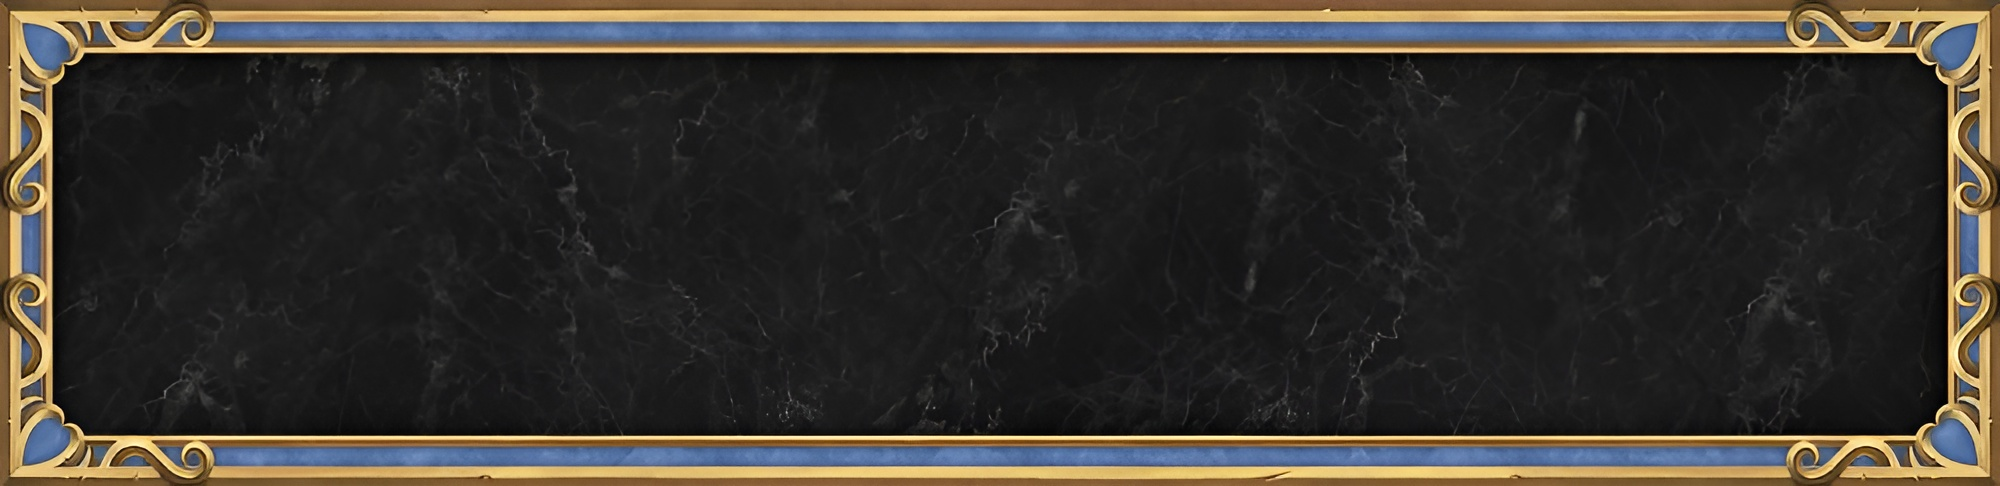
\includegraphics[width=\linewidth, height=0.2\linewidth]{\images/sectionheading.jpg}};
      \draw (-6.2, 0) node {\includegraphics[width=0.125\textwidth]{#2}};
    \end{tikzpicture}
    }
  }
  % \begin{adjustwidth*}{}{0.125\textwidth}
  \begin{fullwidth}[leftmargin=0.16\textwidth]
    \begin{center}
      \fontfamily{ptm}\selectfont{
        \color{antiquewhite} \section*{#1}
      }
      \addcontentsline{toc}{section}{\protect\numberline{}#1}
    \end{center}
  % \end{adjustwidth*}
  \end{fullwidth}
  \vspace{3em}
}
%End of create section heading.

\definecolor{darkcandyapplered}{rgb}{0.64, 0.0, 0.0}

% Command for overlay circled text
\definecolor{goblin}{HTML}{3b7c33}
\newcommand\encircle[1]{%
  \tikz[baseline=(X.base)]
  \node (X) [draw=white, shape=circle, inner sep=0, fill=goblin, text=white, blur shadow={shadow blur steps=5}] {\strut \textbf{#1}};%
}

% Background
\AddToHook{shipout/background}{%
    \put (0in,-\paperheight){
\includegraphics[width=\paperwidth,height=\paperheight]{\images/tausta.png}}%
    \put (0in,-\paperheight){
\includegraphics[width=\paperwidth,height=0.05\paperheight]{\images/bottom.png}}%
}

\begin{document}

\title{
\includegraphics[width=4cm]{\images/title.png} The Rewritening}

\author{Hermanni "Heegu" Karppela}
\maketitle

\begin{center}
Version 0.3
\end{center}

\tableofcontents

\clearpage

\textbf{Heroes of Might and Magic III: The Board Game} is a tactical strategy RPG board game for 1-3 players using the core box set.
The continent of Antagarich is under war as several different factions, led by their Heroes, battle for supremacy. Choose your Faction and your Hero and banish your unruly enemies from these lands!
\bigbreak

% !TeX spellcheck = en_US
\addsection{Game Modes}{\skills/intelligence.png}

\begin{multicols*}{2}

Each game of Heroes III is played using a Scenario from the Mission Book.
There are four types of Scenarios:

\subsection*{Clash}
A fully competitive mode for 2-3 players.

\subsection*{Campaign}
A single player mode of interconnected Scenarios against an enemy AI.
For rules unique to Solo Mode, see \hyperlink{AIrules}{here}.
Further rules changes are detailed in the Campaign Mission Books.

\subsection*{Alliance}
A 2 vs. 2 team-based mode.
You will need an expansion pack to be able to play a 4-player game.

\subsection*{Cooperative}
A Cooperative mode for 2-3 players where everyone shares the same goal.

\vspace*{\fill}

\columnbreak

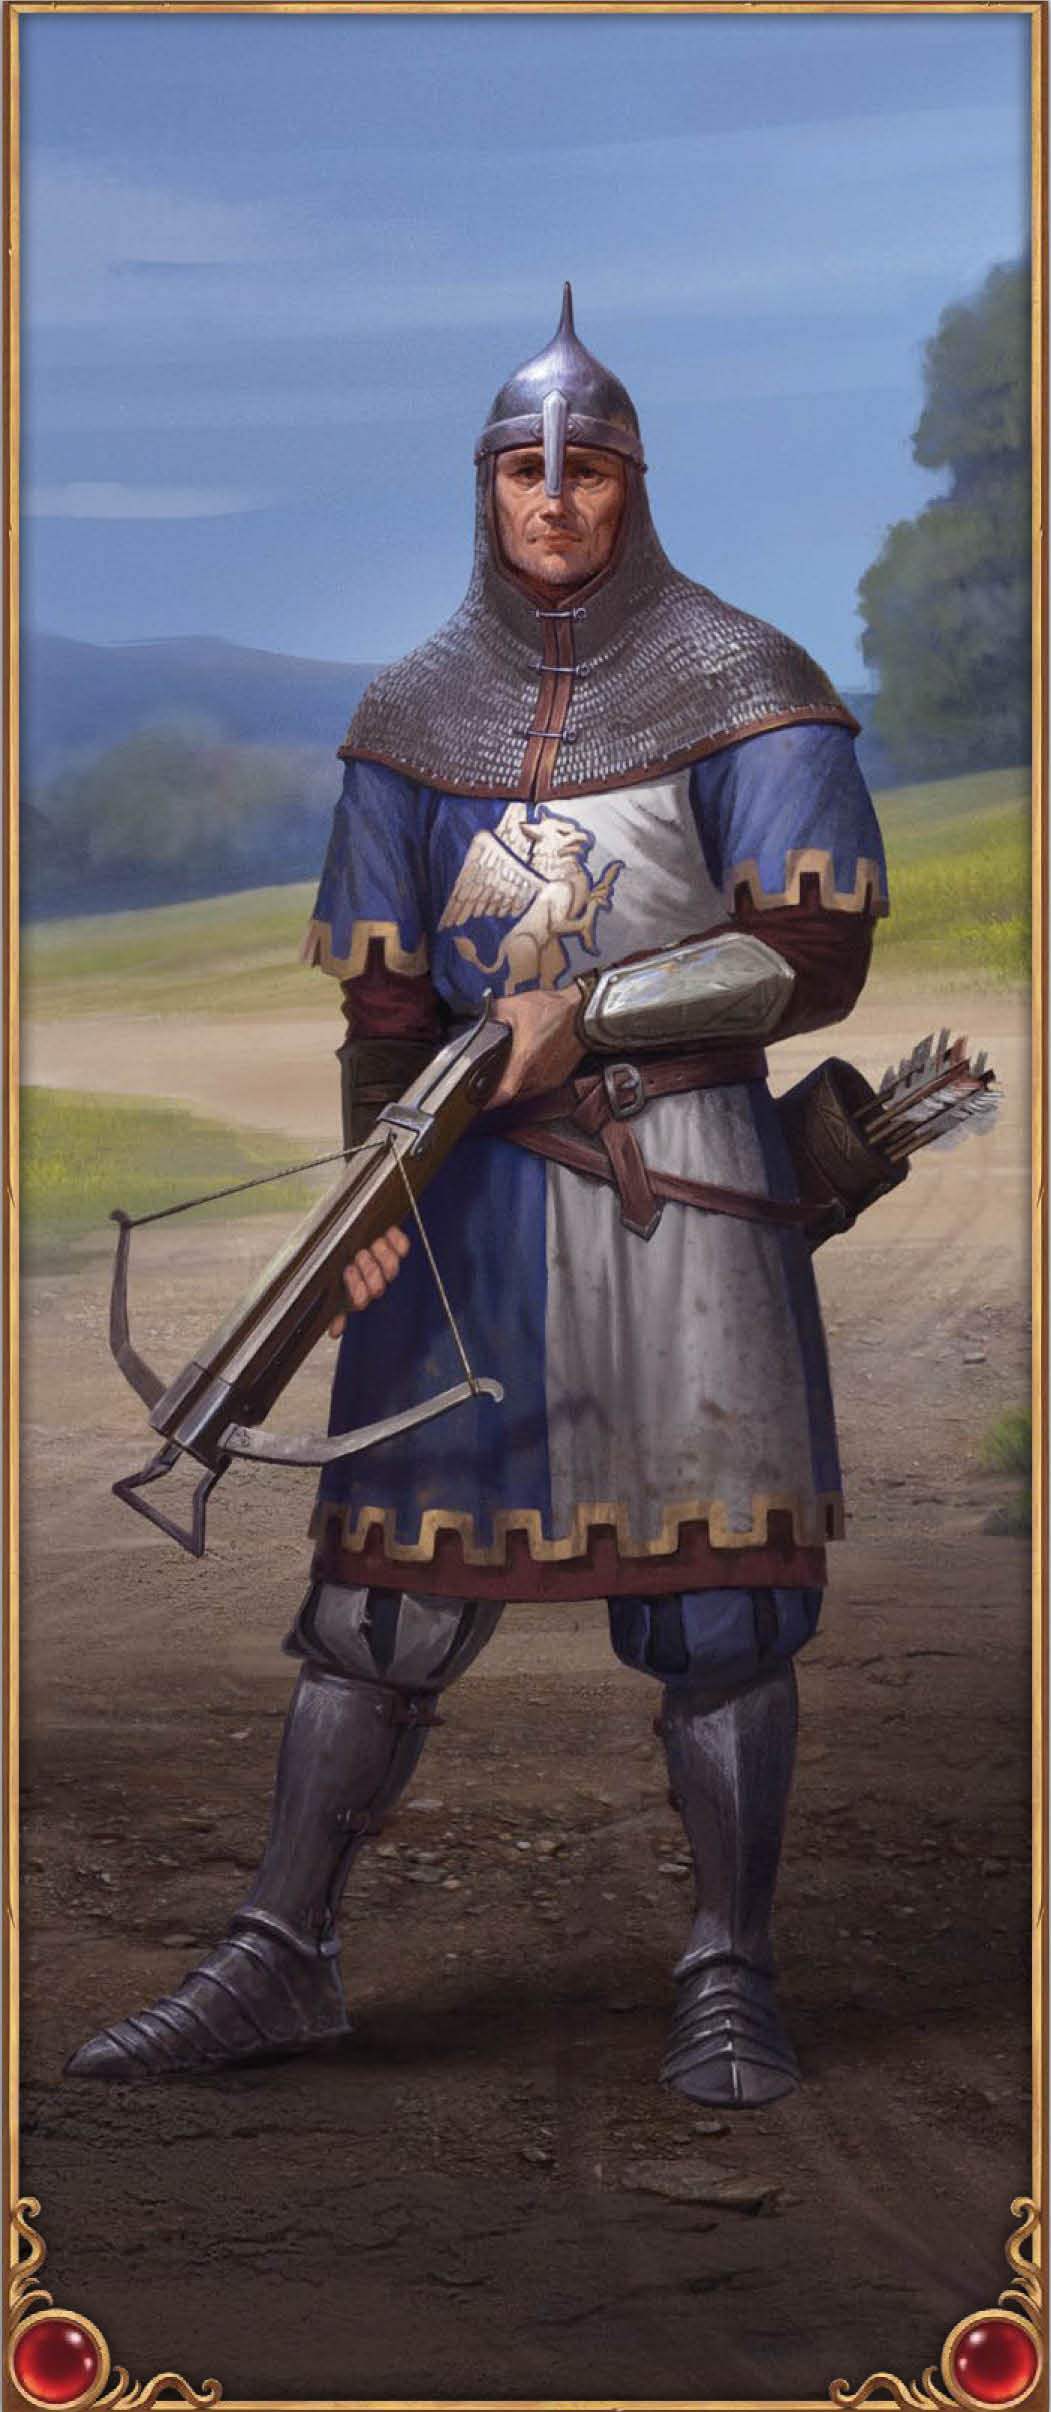
\includegraphics[width=\linewidth]{\art/archer.jpg}

\end{multicols*}


% !TeX spellcheck = en_US
\addsection{Setup}{\skills/necromancy.png}

\begin{multicols*}{2}

This section will guide you through the process of setting up a Scenario from the Mission Book.

\begin{enumerate}
  \item Select a Scenario from the Mission Book.
    For your first game, we recommend choosing the ``Brave New World'' Scenario (see page 7 in the Mission Book).
  \item Choose your Faction from those available.
  \item Choose one of your Faction's Heroes as your Main Hero.
    Each Faction has at least one double-sided Hero Card, with each side depicting a different Hero.
  \item Take the following components belonging to your Faction:
  \begin{itemize}
    \item[a)]1 × Double-sided Hero Card (on the side of the chosen Hero)
    \item[b)]2 × Hero model
    \item[c)]7 × Town Building Tile
    \item[d)]1 × Town Board
    \item[e)]7 × Double-sided Unit Card
    \item[f)]3 × Hero-specific Specialty Card (of the chosen Hero)
    \item[g)]1 × Hero-specific Ability Card (of the chosen Hero)
    \item[h)]20 × Faction Cube
    \item[i)]1 × Build Token
    \item[j)]1 × Population Token
    \item[k)]1 × Spell Book Token
    \item[l)]3 × Movement Tokens
  \end{itemize}
  \item Place one of your Faction Cubes on the first space of the Level Tracker found on the Hero Card (Represented by a ``1'').
    Your hero is now Level 1.
  \item Set up the Map Tiles and other Scenario-specific components as shown in the Mission Book.
  \item Place the Town Board of your chosen Faction in front of you and set the Town Building Tiles next to it.
    Check which Buildings are already built in the Scenario you are about to play, and place the respective Building Tiles on the Town Board.
    Resolve any immediate effects from already built Buildings at the end of the setup.
  \item Set your starting income as indicated by the Scenario by placing your Faction Cubes on the income trackers on your Town Board.
    Place the Population, Build, and Spell Book Tokens in their respective slots on the Town Board.
  \item Group the Resource Tokens into separate piles located within reach of all players.
    Take the starting Resources determined by the Scenario you are playing and place them next to your Town Board.
    This is your Resource pool.
  \item Separate the remaining Tokens into their respective piles.
  \item Sort the Statistic Cards into four piles: Attack, Defense, Power, and Knowledge.
    Refer to the Statistics on your \hyperlink{Herocard}{Hero Card} and take the corresponding number of Cards from each pile.
  \item If your Main Hero is a Hero of Might \includesvg[height=10px]{\svgs/might.svg}, add 1 copy of the Magic Arrow Spell to Your Deck, and if they’re a Hero of Magic \includesvg[height=10px]{\svgs/magic.svg}, add 2 of these Spells to Your Deck.
  \item Add your Hero's \hyperlink{Ability}{Ability} and Level 1 \hyperlink{Specialty}{Specialty} Cards to your Starting Deck.
  \item Shuffle your Starting Deck and place it face down next to your Hero Card.
    This Deck is your Main Hero's \textbf{Deck of Might \& Magic}\index{Deck of Might \& Magic}, and is now ready. In this rule book, this is shortened to \textbf{Your Deck}.
  \item Sort the Ability, Artifact, and Spell Cards into 3 face down Decks (including any unused Magic Arrow Spells) and shuffle them.
    From each of these Decks, take the top Card and place it face up next to its Deck, creating 3 separate Discard Piles.
  \item Choose the Scenario's \hyperlink{Difficulty}{Difficulty} and take the corresponding Starting Bonus(es).
  \item Sort the Neutral Units into 4 Decks according to their tier (\includesvg[height=10px]{\svgs/bronze.svg}\includesvg[height=10px]{\svgs/silver.svg}\includesvg[height=10px]{\svgs/golden.svg}\includesvg[height=10px]{\svgs/azure.svg}).
    Shuffle these Decks and leave enough room for their Discard Piles.
  \item Place the Combat Board within reach of the players.
    Check the Scenario for which starting Units you receive and place them into a pile near your Town Board, separate from the rest of your Faction’s Units.
  \item Place the Round Tracker next to the game map and place a Black Cube on the ``1'' space.
  \item Shuffle the Astrologers Proclaim Cards and place them face down next to the Round Tracker.
  \item Orientate your Starting Tile to your liking.
    Choose which Hero model represents your Main Hero in this game and place the chosen model on the center Field of your Starting Tile.
  \item Choose a starting player. The starting player never changes during the game.
\end{enumerate}

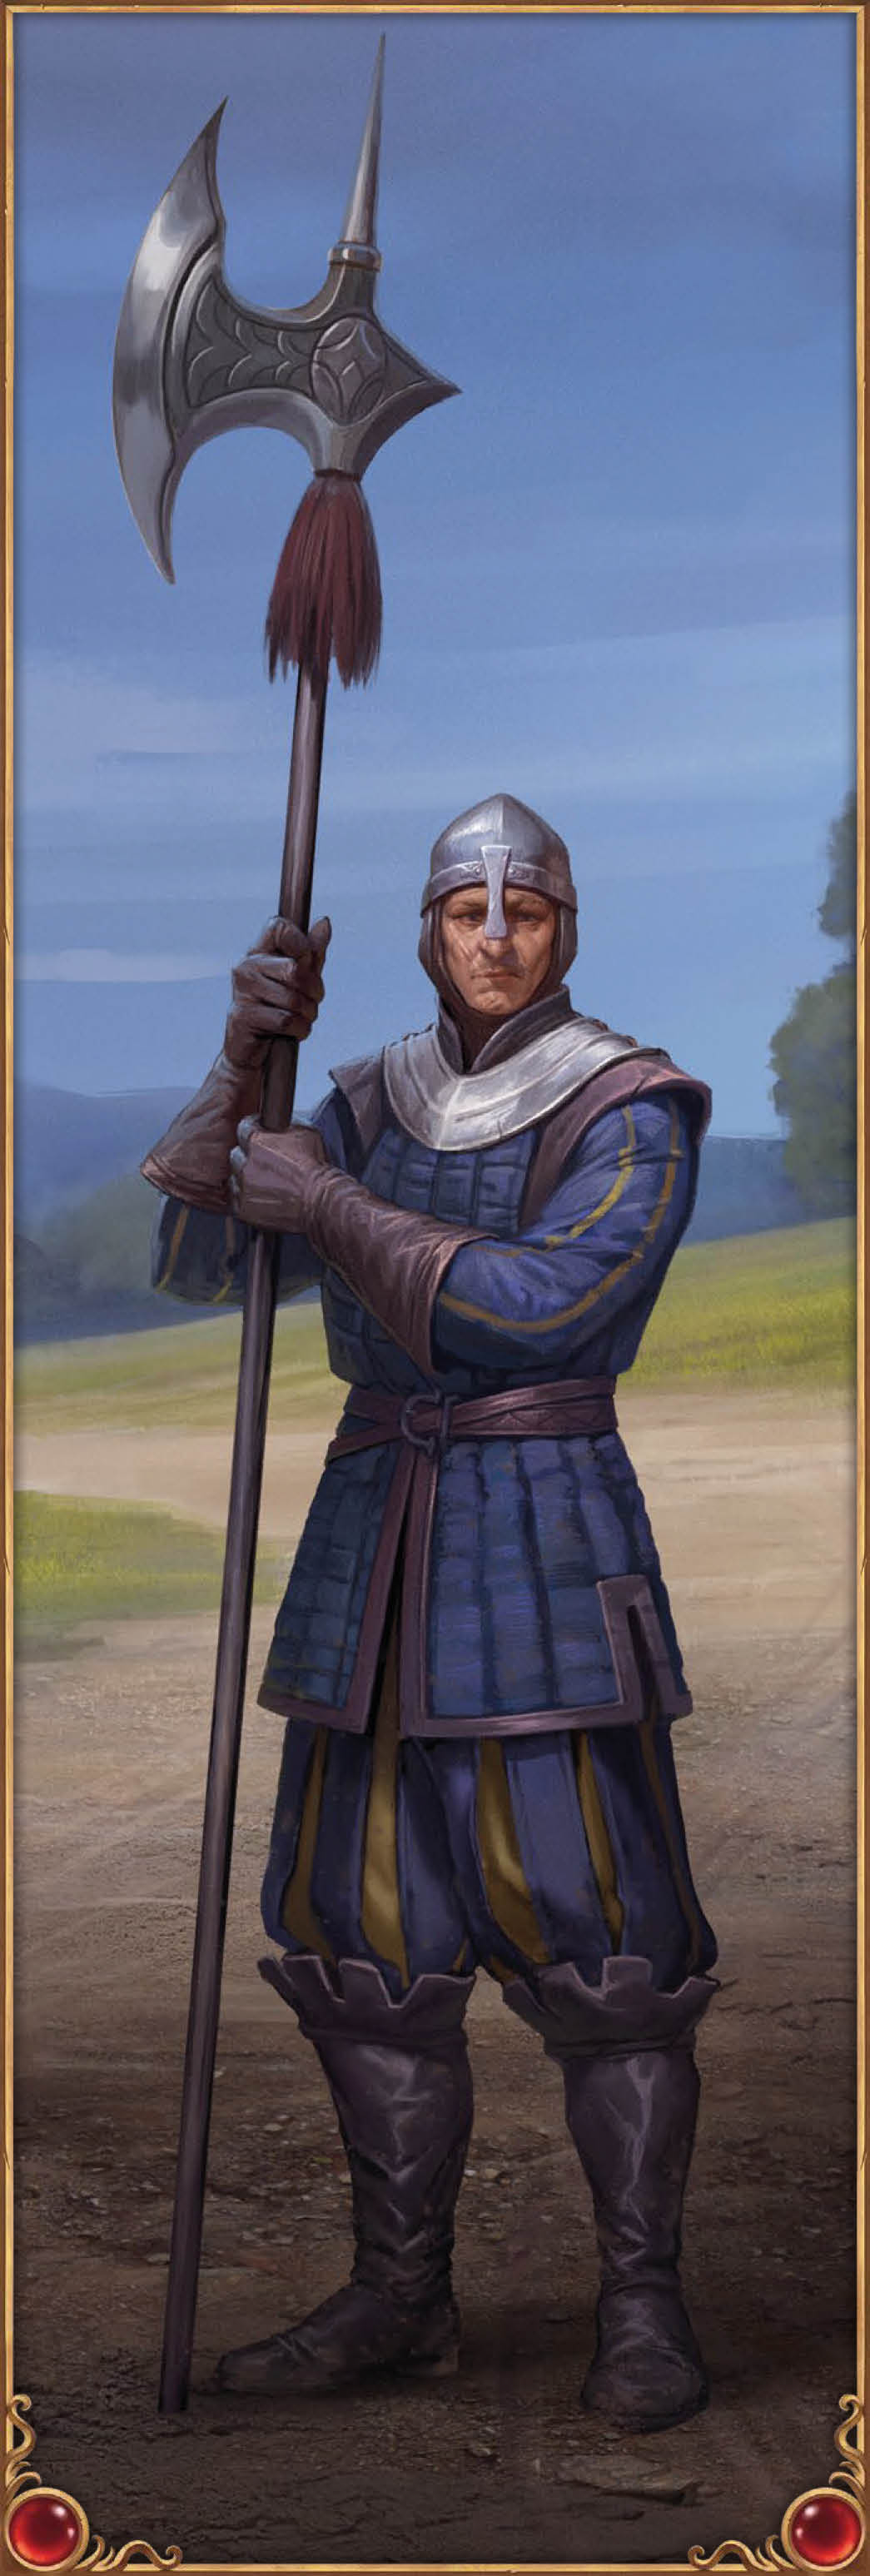
\includegraphics[width=\linewidth]{\art/halberdier.jpg}

\vspace*{\fill}

\end{multicols*}

\begin{figure}[h]
  \centering
  \begin{scriptsize}
  \begin{tikzpicture}
    \draw (0, 0) node[inner sep=0] {\makebox[\textwidth][c]{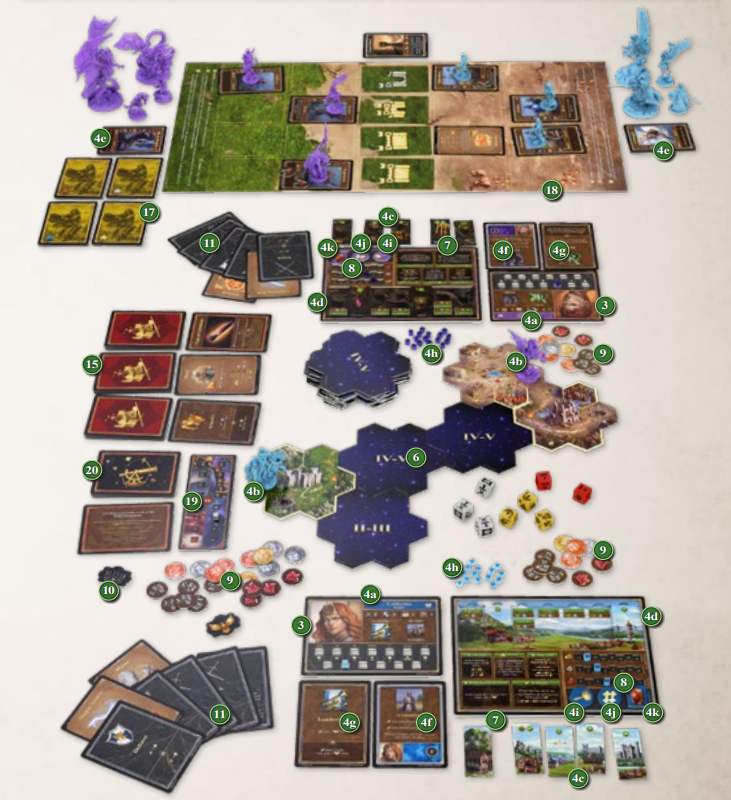
\includegraphics[width=1.25\linewidth]{\images/setup.png}}};
    \draw (6.2, 2.9) node {\encircle{\phantom{.}3\phantom{.}}};
    \draw (-1.8, -5.5) node {\encircle{\phantom{.}3\phantom{.}}};
    \draw (0, -4.7) node {\encircle{4a}};
    \draw (4.3, 2.4) node {\encircle{4a}};
    \draw (-3.1, -1.7) node {\encircle{4b}};
    \draw (3.9, 1.4) node {\encircle{4b}};
    \draw (5.5, -9.6) node {\encircle{4c}};
    \draw (0.5, 5.2) node {\encircle{4c}};
    \draw (7.3, -5.5) node {\encircle{4d}};
    \draw (-1.3, 2.9) node {\encircle{4d}};
    \draw (-7.1, 7.5) node {\encircle{4e}};
    \draw (7.5, 7) node {\encircle{4e}};
    \draw (1.3, -7.9) node {\encircle{4f}};
    \draw (3.7, 4.4) node {\encircle{4f}};
    \draw (-0.5, -7.9) node {\encircle{4g}};
    \draw (5, 4.4) node {\encircle{4g}};
    \draw (1.6, 1.7) node {\encircle{4h}};
    \draw (1.9, -4.3) node {\encircle{4h}};
    \draw (5.5, -7.9) node {\encircle{4i}};
    \draw (0.5, 4.4) node {\encircle{4i}};
    \draw (6.3, -7.9) node {\encircle{4j}};
    \draw (-0.1, 4.4) node {\encircle{4j}};
    \draw (7.3, -7.9) node {\encircle{4k}};
    \draw (-1.2, 4.5) node {\encircle{4k}};
    \draw (2.6, 2.0) node {\encircle{4l}};
    \draw (7.0, -4.3) node {\encircle{4l}};
    \draw (1.4, -1.3) node {\encircle{\phantom{.}6\phantom{.}}};
    \draw (3.1, -8.1) node {\encircle{\phantom{.}7\phantom{.}}};
    \draw (2.2, 4.4) node {\encircle{\phantom{.}7\phantom{.}}};
    \draw (6.5, -6.9) node {\encircle{\phantom{.}8\phantom{.}}};
    \draw (-0.5, 3.8) node {\encircle{\phantom{.}8\phantom{.}}};
    \draw (-3.1, -4.5) node {\encircle{\phantom{.}9\phantom{.}}};
    \draw (6.3, -3.6) node {\encircle{\phantom{.}9\phantom{.}}};
    \draw (6.1, 1.6) node {\encircle{\phantom{.}9\phantom{.}}};
    \draw (-6.6, -4.5) node {\encircle{10}};
    \draw (-4, 4.5) node {\encircle{11}};
    \draw (-4, -7.5) node {\encircle{11}};
    \draw (-7.1, 1.5) node {\encircle{15}};
    \draw (-5.6, 5.5) node {\encircle{17}};
    \draw (5.1, 5.8) node {\encircle{18}};
    \draw (-4.8, -2) node {\encircle{19}};
    \draw (-7.1, -1.5) node {\encircle{20}};
  \end{tikzpicture}
  \end{scriptsize}
\end{figure}


\addsection{Round Structure}{\images/forgetfulness.png}

\begin{multicols*}{2}

The game is structured into Rounds, during which each player will take their own Turn in a clockwise order starting with the starting player.
During their turns, players will move their \hyperlink{Heroes}{Heroes} on the Game Map, construct new Buildings in their \hyperlink{Town}{Town} and Recruit \hyperlink{Units}{Units} in an attempt to fulfill the Scenario's victory condition.\par
Perform the following steps at the start of every Round except the first one:
\begin{itemize}
  \item Flip any previously used Build, Population and/or Spell Book Tokens back to their active side.
  \item Flip any previously used Movement Point (MP) Tokens back to their active, green side.
  \item Regain uses for Expert Effects \includesvg[height=10px]{\svgs/expert.svg}.
\end{itemize}
Then, depending on the current Round number, players either gain Resources or resolve an Astrologers Proclaim card:
\begin{itemize}
  \item Odd-numbered rounds are Resource Rounds.
    All players gain income from the \hyperlink{Mines}{Buildings, Settlements, and Mines} they control.
    Skip this step during the first round.
  \item Even-numbered rounds are Astrologers' Rounds.
    Draw an Astrologers Proclaim card and resolve its effects.
  \item If the Scenario has timed events marked on the round tracker that have now been reached, resolve them.
\end{itemize}
\subsection*{Player Actions}
\begin{itemize}
  \item During their turn, players spend their Movement Points (MP) to perform actions with their Heroes.
  \item Build, Population and Spell Book Tokens may be used at any point during any player's turn except during Combat.
  \item Once all players have performed their turn, move the Black Cube on the Round Tracker and perform the start of Round again.
\end{itemize}
Keep playing new Rounds until any of the Scenario's ending conditions have been met.

\vfill
\hspace{2em}
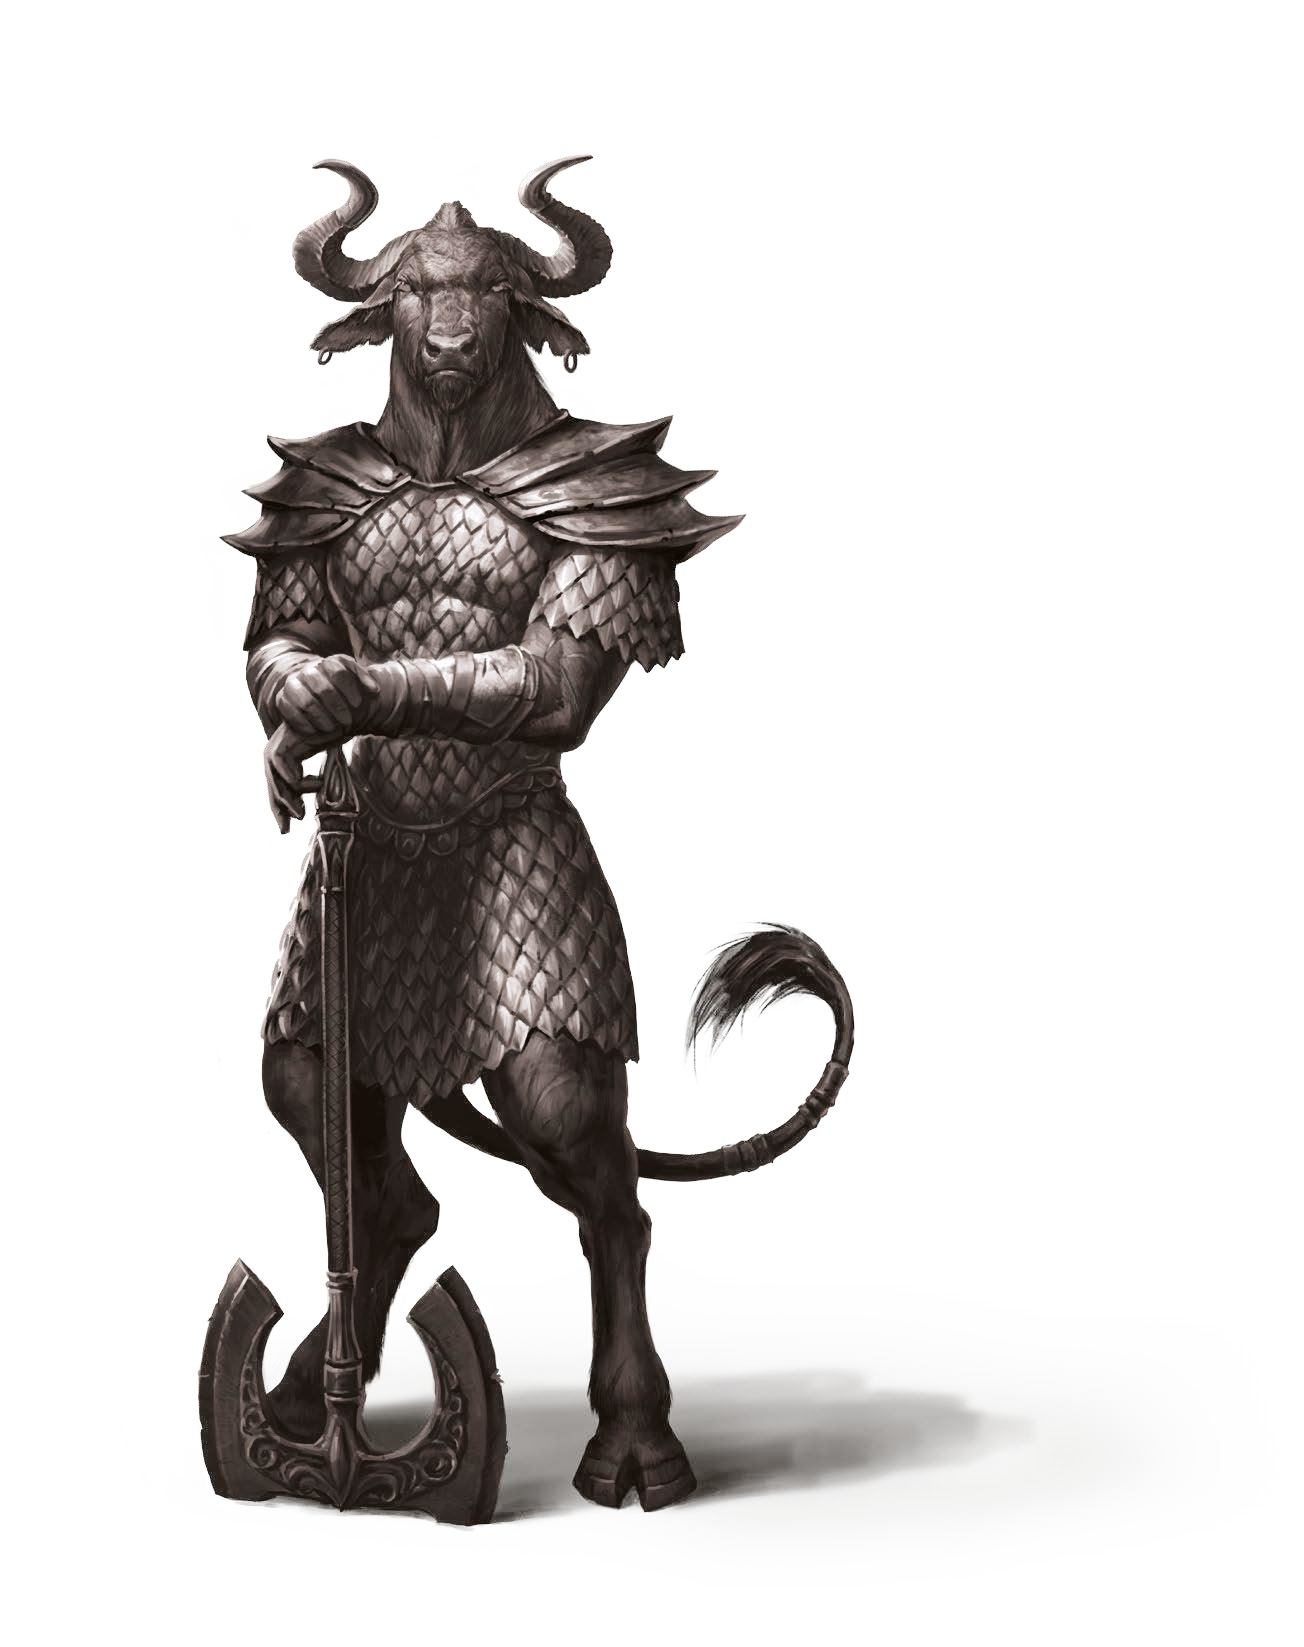
\includegraphics[scale=0.2]{\art/minotaur.png}
\vfill

\end{multicols*}


% !TeX spellcheck = en_US
\addsection{Player Turns}{\spells/dimension_door.png}

\begin{multicols}{2}

At the start of a player's Turn, that player refreshes their hand of Cards from their Deck of Might \& Magic following two steps in order:
\begin{itemize}
  \item Discard any number of Cards from your hand.
If your current hand exceeds your Hand Limit \includesvg[height=10px]{\svgs/hand.svg}, you must discard down to at least your Hand Limit.
  \item Draw back to your Hand Limit.
\end{itemize}
Your current Hand Limit depends on your Main Hero's \hyperlink{Level}{Level}.
The beginning of your Turn is the only time your Hand Limit is checked.\par
There are three types of Actions players may take during their Turn: \textbf{Movement}, \textbf{Town} and \textbf{Morale} Actions.
Once all players have spent all their Movement Points on their Turns and do not wish to use any further Town or Morale Actions, the current Round is over.
\subsection*{Movement Actions}
\hypertarget{Movement}{Movement Actions}\index{Movement Actions} are performed by spending Movement Points.
A player can use Movement Actions \textbf{only during their own Turn}.\par
For every 1 MP spent, you can perform one of the following Actions:
\begin{itemize}
  \item Move a Hero 1 Field in any direction.
  \item \hyperlink{Categories}{Revisit} a Field where your Hero is in.
  \item \hyperlink{Timelimit}{Continue Combat} against Neutral Units for 1 additional Combat Round.
  \item \hyperlink{Placing}{Discover a face down Map Tile} if your Hero is on a Field next to that Tile.
  \item Place a new Map Tile from your pool of Far (II-III) Map Tiles.
\end{itemize}

\begin{center}
  \includesvg[width=0.6\linewidth]{\images/movement_tokens.svg}\\
  \medskip
  \footnotesize\textit{An active and an inactive Movement Token.}
\end{center}

\bigskip

Mark the amount of MP you have used by flipping your Movement Tokens over to their brown, inactive side.
If a player has both a Main and a \hyperlink{Secondary}{Secondary Hero}, track their MP separately.
Heroes can spend MP in any order.\par
Allied Heroes can move through each other but cannot stop their movement in the same Field.
When you move through a Field with an allied Hero, do not \hyperlink{Categories}{Visit} the Field that the allied Hero is standing on.\par
\note{10}{
  Whenever you are instructed to gain (additional) MP, sometimes represented by the symbol \includesvg[height=10px]{\svgs/movement-note.svg}, that MP persists for \textbf{only the Turn it was gained on}.
  In the unlikely situation that two allied Heroes are forced onto the same Field, you must use your next MP to move one of them away from that Field.
}

\vfill
\begin{center}
  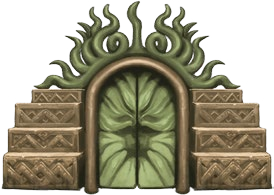
\includegraphics[width=0.8\linewidth]{\art/town_portal.png}
\end{center}

\clearpage

\subsection*{Town Actions\index{Town Actions}}
You can perform each of the Town Actions listed below \textbf{once per Round}.
These Actions can be performed at any point during any player's Turn, except during Combat or when a player is resolving an Action that would be interrupted by your Town Action.
For example, you cannot draw Spell cards simultaneously with the Spell Book Token.\par
When a player announces that they are about to start Combat, you may react to it with any number of Town Actions before performing any of the steps of \hyperlink{Combatsetup}{setting up Combat.}\par
If multiple players wish to use a Town Action at the same time and the order of resolving them has an effect on the game, you may roll an Attack or Resource Die and let the highest roller perform the Action first.\par
After performing a Town Action, flip the respective Token on its inactive side on your Town Board.
You cannot use that Action again until the start of the next Round, when the Tokens are refreshed.
\begin{itemize}
  \item [{
\includegraphics[height=1.5\baselineskip, valign=c]{\images/build.png}}] Build Token, used to expand your \hyperlink{Town}{Town}.
  \item [{
\includegraphics[height=1.5\baselineskip, valign=c]{\images/population.png}}] Population Token, used to Recruit and Reinforce \hyperlink{Units}{Units} or to Recruit \hyperlink{Secondary}{a Secondary Hero}.
  \item [{
\includegraphics[height=1.5\baselineskip, valign=c]{\images/spells.png}}]Spell Book Token, used to purchase \hyperlink{spells}{Spells}.
\end{itemize}

\subsection*{Morale Actions}\index{Morale Actions}
Players can gain or lose Morale through various game effects.
When you gain Morale, take a Positive Morale Token\index{Positive Morale} \includesvg[height=10px]{\svgs/positive.svg}.
You may only have one such Token.
If you would gain a second Token, you may immediately spend the first one before gaining the second.
A Positive Morale Token may be spent to perform any of the following Actions at any time:
\begin{itemize}
  \item Draw a Card from your Deck.
  \item Discard any number of Cards, then draw that many Cards.
  \item Reroll any Die you have thrown.
\end{itemize}
If you lose Morale, discard a Positive Morale Token \includesvg[height=10px]{\svgs/positive.svg} if you have one, otherwise gain a Negative Morale\index{Negative Morale} Token \includesvg[height=10px]{\svgs/negative.svg}.
Inversely, gaining Positive Morale while you have a Negative Morale Token discards the Token.
If you would gain a second Negative Morale Token, you must instead \textbf{discard your hand of Cards} the next time you end your Turn.\par

\note{5}{The Necropolis \includesvg[height=10px]{\svgs/necro-note.svg} Faction ignores any Morale effects.
  They cannot ever gain or lose Morale for any reason.
}

\begin{center}
  
\includegraphics[width=\linewidth]{\art/shield.png}
\end{center}

\subsection*{Example Turn}

\textit{Alice, who is playing the Hero Catherine the Knight, begins her Turn.
She has 3 cards in her hand from the previous round, and decides to discard 2 of them before drawing cards from her Deck up to her Hand Limit \includesvg[height=10px]{\svgs/hand.svg}.
The current limit is 5, since her Main Hero is Level 3, so she draws 4 cards after discarding (see \hyperlink{Level}{Level Effects}).}\par
\textit{She then spends her Build Token to construct the \includesvg[height=10px]{\svgs/golden.svg} Dwelling, and then her Population Token to \hyperlink{Units}{Recruit} the \includesvg[height=10px]{\svgs/golden.svg} Unit Champions.
She is allowed to do this, as she had previously built the prerequisite lower Level Dwellings (\includesvg[height=10px]{\svgs/bronze.svg} and \includesvg[height=10px]{\svgs/silver.svg}) and has enough \hyperlink{Resources}{Resources} to both Build the Dwelling and to Recruit the Champions.}\par
\textit{Now prepared for a coming battle, she spends a Movement Point to move her Main Hero to an adjacent Field currently occupied by Sandro the Necromancer, an enemy Main Hero controlled by Bob.
As Alice announces her intent to start Combat, both players still now have an opportunity to perform Town Actions.}\par

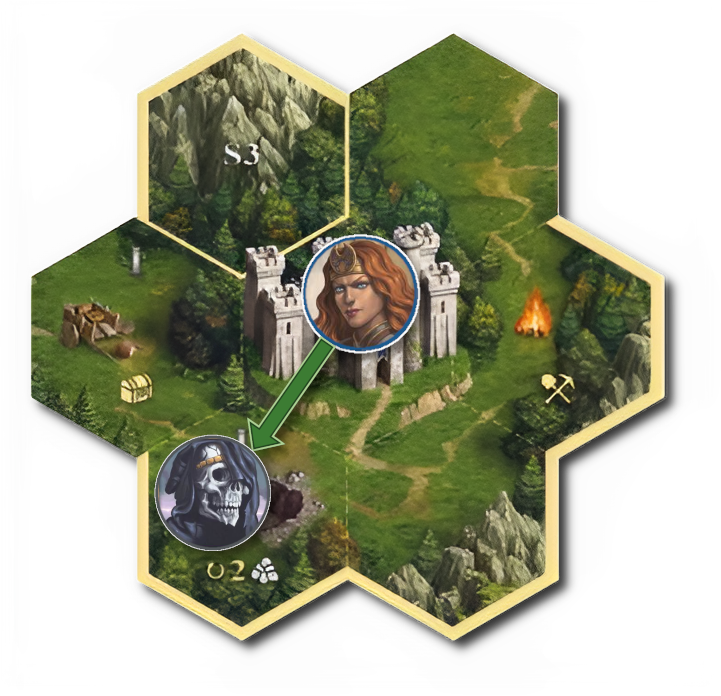
\includegraphics[width=\linewidth]{\examples/catherine_attacks_sandro.png}

\end{multicols}

\vfill

\begin{figure*}[!hb]
  \centering
  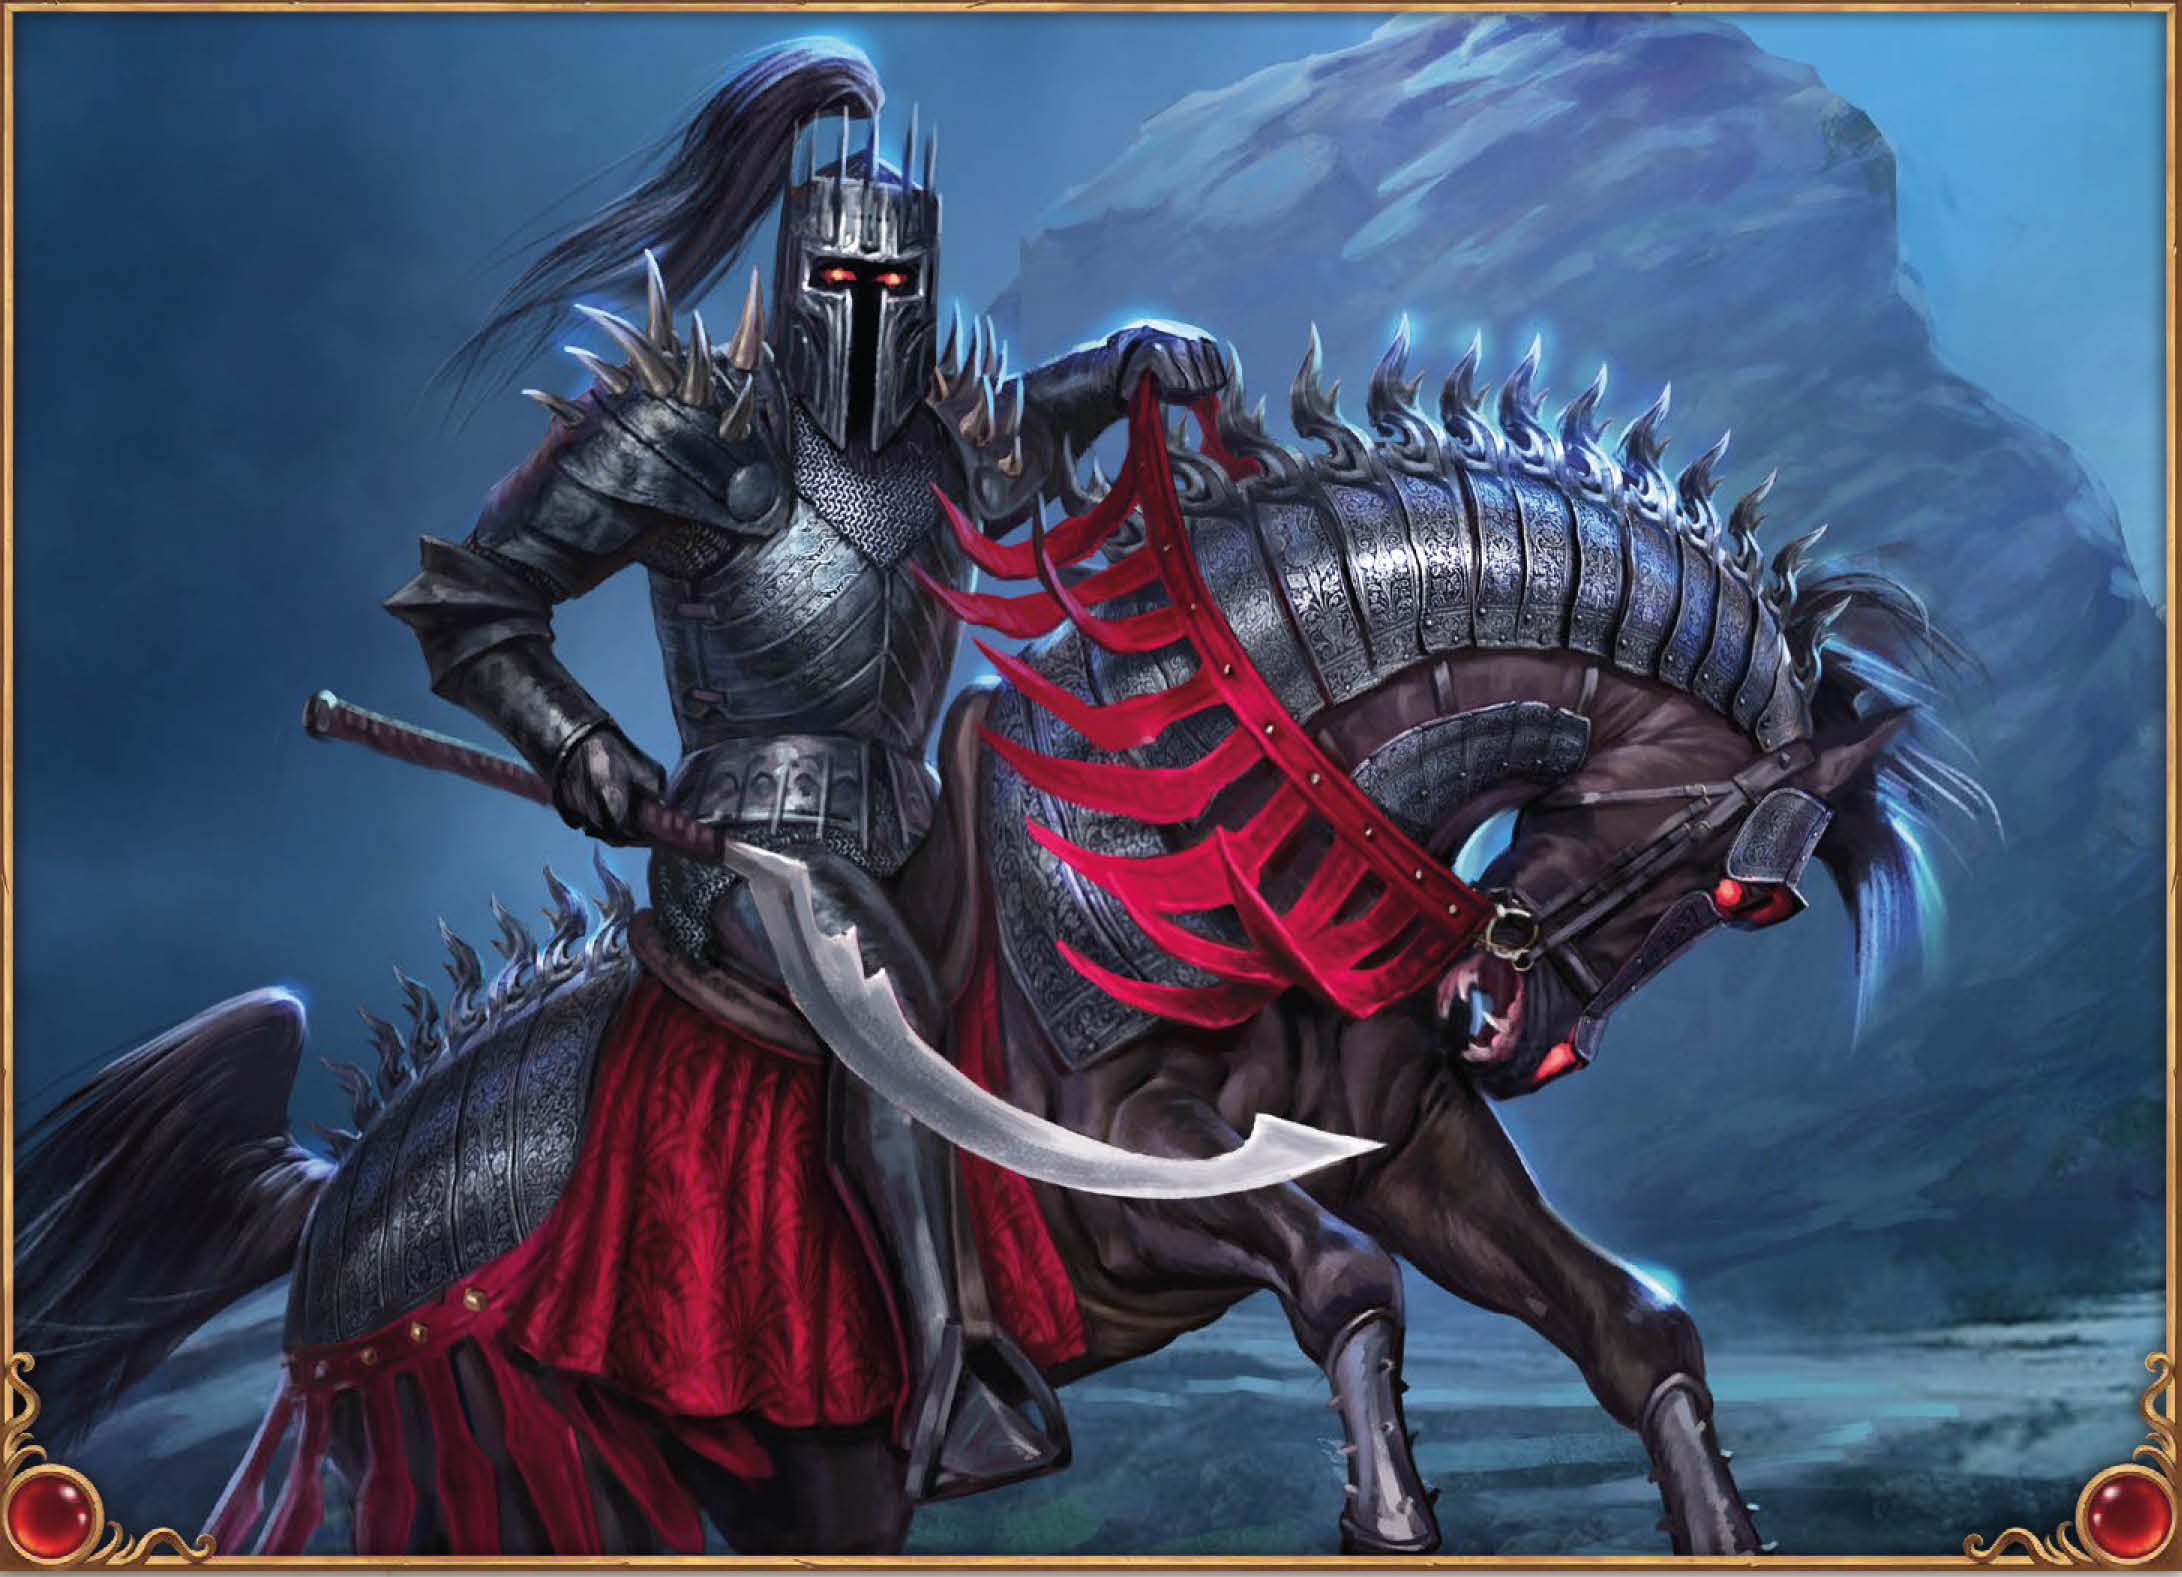
\includegraphics[width=\linewidth]{\art/dread_knight.jpg}
\end{figure*}
\vfill


% !TeX spellcheck = en_US
\addsection{Heroes}{\skills/sorcery.png}

\begin{multicols*}{2}

\hypertarget{Heroes}{Players} always control a Main Hero and may additionally also recruit a Secondary Hero.
A "player's Hero" may refer to either of them.
Heroes are used to perform Movement Actions on the game board and to start Combats against enemies in order to reach a Scenario victory condition.

\subsection*{Main Hero}
The Main Hero\index{Main Hero} is represented by its chosen model, Hero Card and Your Deck.
Each Faction's Main Hero has 3 Movement Points.
Only the Main Hero can use Your Deck.\par
Each Main Hero starts the game at Level 1 and can advance up to Level 7 by gaining Experience.
Experience is gained from \hyperlink{Combatexperience}{winning Combat}, Visiting certain \hyperlink{All}{Locations} and the \hyperlink{Resources}{Treasure Die} \includesvg[height=10px]{\svgs/treasure.svg}.
Gaining 1 Experience\index{Experience} is represented by the symbol \includesvg[height=10px]{\svgs/exp.svg}.

\subsection*{\hypertarget{Secondary}{Secondary Heroes}}
If you control a Town or a Settlement, a Secondary Hero\index{Secondary Hero} can be Hired by flipping your \textbf{Population Token} and paying 10 Gold \includesvg[height=10px]{\svgs/gold.svg}.\par
\note{5}{Units \textbf{cannot} be \hyperlink{Units}{Recruited or Reinforced} while using the Population Token to recruit a Secondary Hero.}\par
Your Secondary Hero uses the remaining Hero model of your Faction.
You may wish to mark this model with a token such as a Faction Cube to differentiate it from the Main Hero.
After Hiring a Secondary Hero, place the model in a Town or Settlement you control.
\textbf{You can only have one Secondary Hero at a time}.\par
Secondary Heroes have \textbf{2 Movement Points}; when you gain one, take an additional set of 2 Movement Tokens to represent their MP.
They do not have their own Hero Card, \textbf{cannot gain Experience}, and \textbf{cannot use Cards from Your Deck} for any reason.
If a Secondary Hero gains any Cards, place them into your hand as normal (see \hyperlink{Playerdecks}{Deck-building}).
Secondary Heroes are considered to have the same Level as the Main Hero for the purposes of resolving \hyperlink{Quick}{Quick Combat}.\par
If your Secondary Hero is attacked by an enemy Hero, you can choose to have that Hero be \hyperlink{Endcombat}{instantly defeated instead of fighting a Combat}.
When a Secondary Hero is defeated, remove them from the game.
They can be Recruited again with another use of the Population Token.\par

\vfill

\hspace{2em}
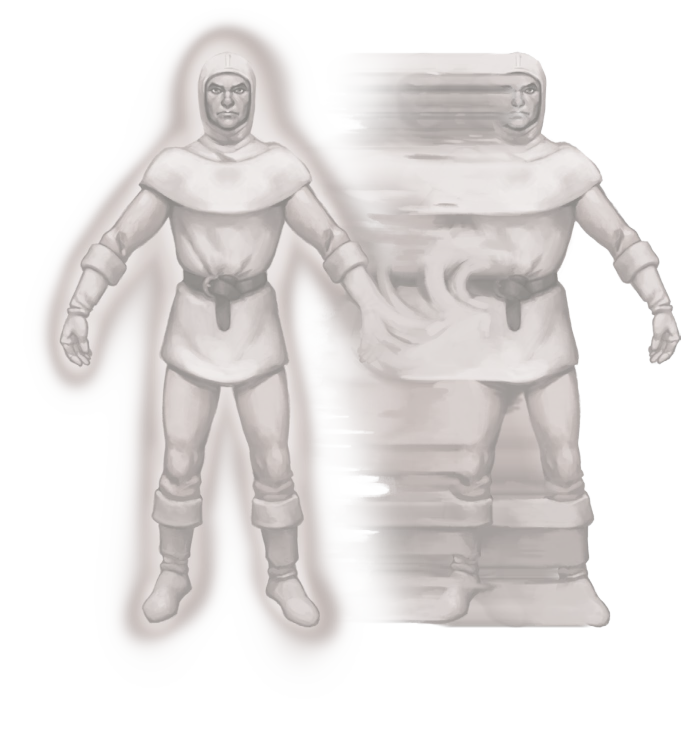
\includegraphics[width=\linewidth]{\art/clone.png}

\end{multicols*}

\clearpage

\subsection*{\hypertarget{Herocard}{Hero Card Anatomy}}\index{Hero Card}
\bigbreak
\begin{figure}[h]
  \begin{minipage}[t]{0.5\textwidth}
    \vspace{0pt}
    \begin{enumerate}[itemsep=5pt]
      \item \textbf{Name} – The Hero's name.
        Used for identification.
        Has no gameplay effect.
      \item \textbf{Class} – The Hero's class.
        Has no gameplay effect.
      \item \textbf{Type} – The Hero's type (Might \includesvg[height=10px]{\svgs/might.svg} or Magic \includesvg[height=10px]{\svgs/magic.svg}).
        Determines the amount of Magic Arrow Spells in your Starting Deck (1 or 2 respectively).
      \item \textbf{Faction Color} – Reminder for the color of the Faction's cubes and miniatures.
      \item \textbf{Attack} – Number of Attack Cards in your Starting Deck.
      \item \textbf{Defense} – Number of Defense Cards in your Starting Deck.
      \item \textbf{Power} – Number of Power Cards in your Starting Deck.
      \item \textbf{Knowledge} – Number of Knowledge Cards in your Starting Deck.
      \item \textbf{Starting Ability} – Reminder for the unique Ability Card\index{Ability Card} the Hero starts with.
      \item \textbf{Hero Specialty} – Reminder for the Specialty Cards the Hero adds to their deck at the start of the game and after specific Level ups.
        Each hero has three Specialty Cards.
      \item \textbf{Level Tracker} – Whenever a Main Hero gains 1 or more Experience \includesvg[height=10px]{\svgs/exp.svg}, move the cube that number of steps on this track.
        When the cube reaches the next slot on the upper row, the hero gains a Level.
    \end{enumerate}
  \end{minipage}\hfill
  \begin{minipage}[t]{0.48\textwidth}
    \centering
    \vspace{0pt}
    \begin{scriptsize}
      \hspace*{2em}
      \begin{tikzpicture}
        \draw (0, 0) node[inner sep=0] {\makebox[\textwidth][c]{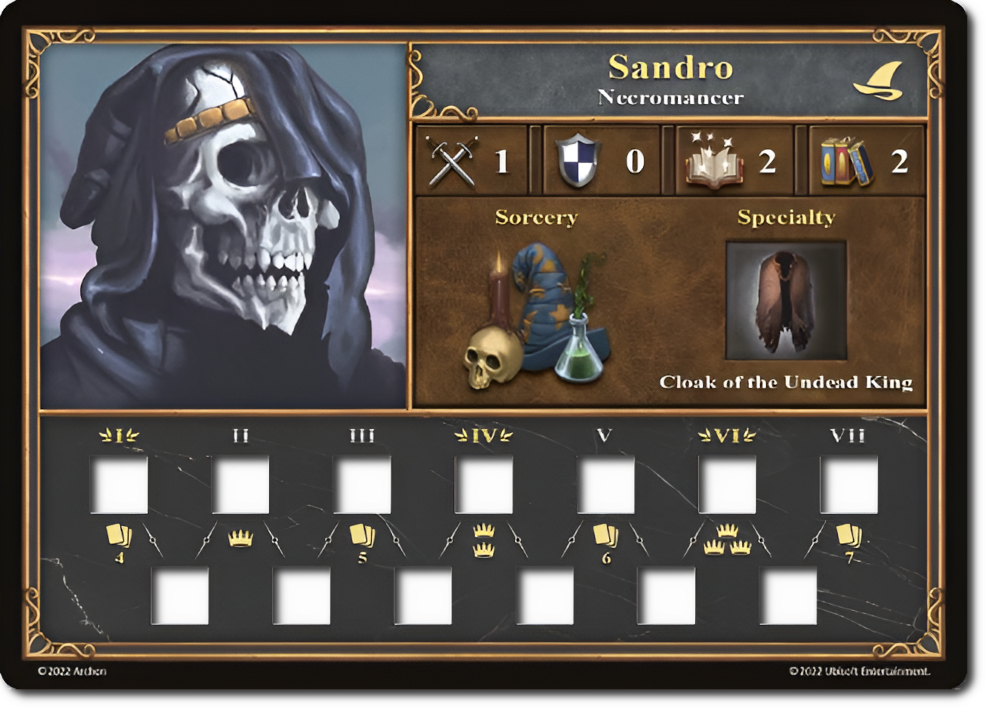
\includegraphics[width=\linewidth]{\cards/hero.png}}};
        \draw (2.2, 2.5) node {\encircle{\phantom{.}1\phantom{.}}};
        \draw (0.8, 1.9) node {\encircle{\phantom{.}2\phantom{.}}};
        \draw (3.5, 2.5) node {\encircle{\phantom{.}3\phantom{.}}};
        \draw (-0.1, 2.5) node {\encircle{\phantom{.}4\phantom{.}}};
        \draw (0, 1.25) node {\encircle{\phantom{.}5\phantom{.}}};
        \draw (1.1, 1.25) node {\encircle{\phantom{.}6\phantom{.}}};
        \draw (2, 1.25) node {\encircle{\phantom{.}7\phantom{.}}};
        \draw (3.25, 1.25) node {\encircle{\phantom{.}8\phantom{.}}};
        \draw (1, -0.2) node {\encircle{\phantom{.}9\phantom{.}}};
        \draw (3, -0.2) node {\encircle{10}};
        \draw (-1.7, -1.4) node {\encircle{11}};
      \end{tikzpicture}
    \end{scriptsize}
    \break
    \footnotesize{\textbf{\textit{\textcolor{darkcandyapplered}{Hero Card}}}}
    \scriptsize
    \begin{multicols}{2}
      \begin{itemize}
        \item[\textbf{1.}] \textbf{Name}
        \item[\textbf{2.}] \textbf{Class}
        \item[\textbf{3.}] \textbf{Type}
        \item[\textbf{4.}] \textbf{Faction Color}
        \item[\textbf{5.}] \textbf{Attack}
        \item[\textbf{6.}] \textbf{Defense}
        \item[\textbf{7.}] \textbf{Power}
        \item[\textbf{8.}] \textbf{Knowledge}
        \item[\textbf{9.}] \textbf{Starting Ability}
        \item[\textbf{10.}] \textbf{Specialty}
        \item[\textbf{11.}] \textbf{Level Tracker}
        \item[\textbf{\phantom{.}}] \phantom{.}
      \end{itemize}
    \end{multicols}
  \end{minipage}
\end{figure}

\begin{tikzpicture}[overlay]
  \node at (12, -0.5) {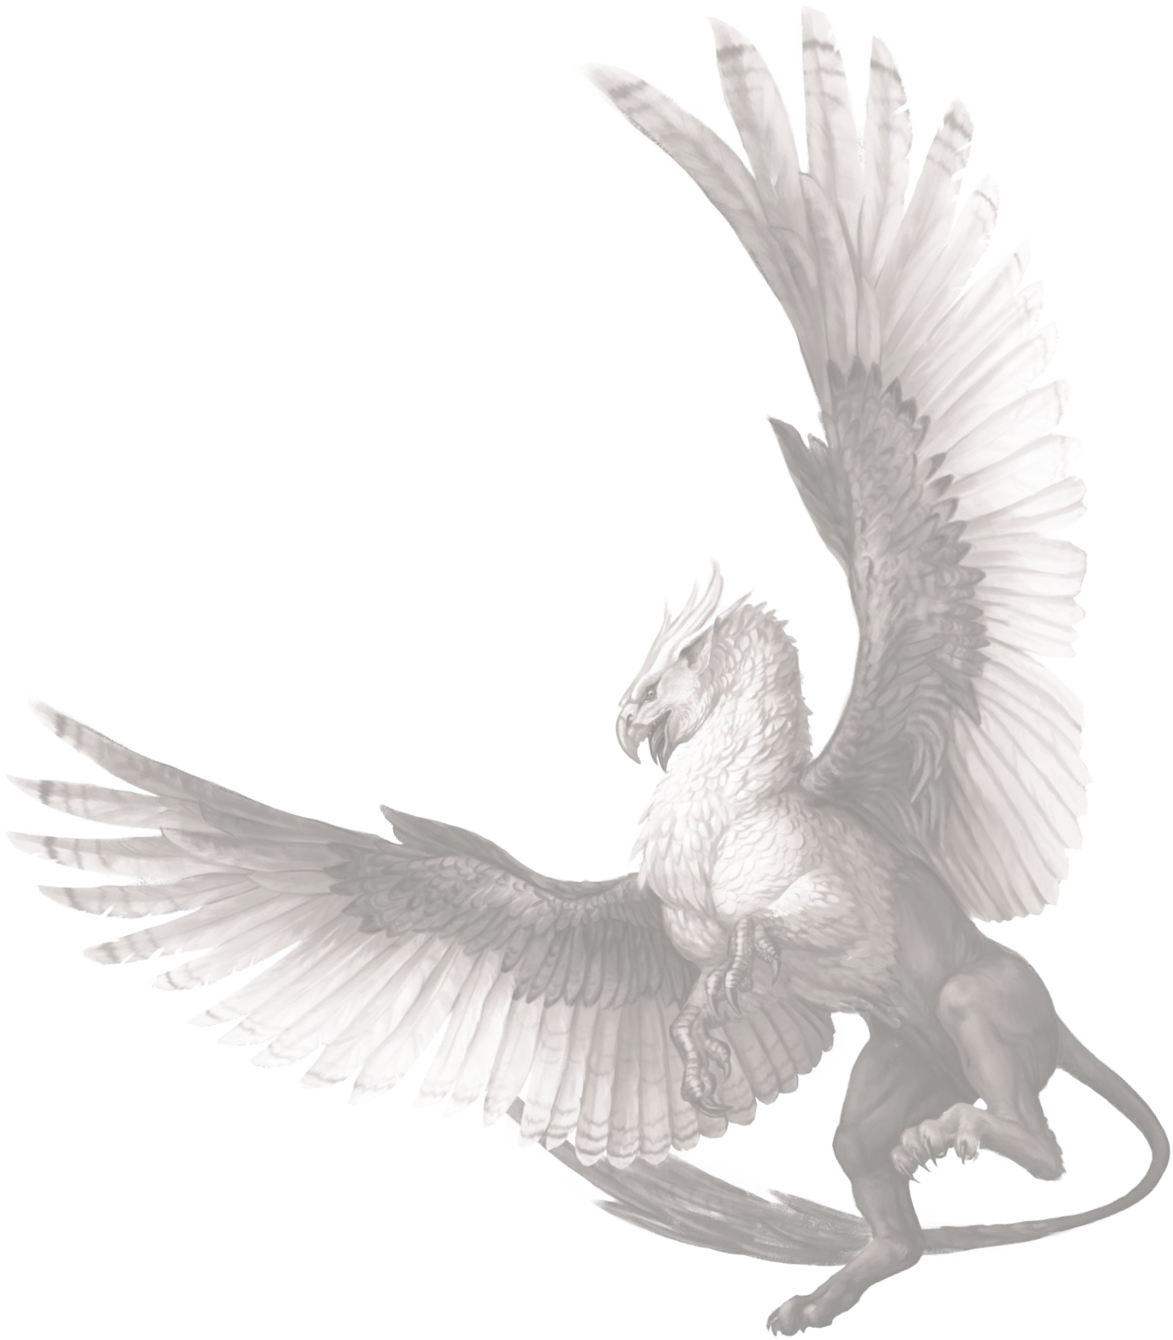
\includegraphics[width=0.6\linewidth]{\art/griffin.png}};
\end{tikzpicture}

\clearpage

\begin{multicols}{2}

\subsection*{\hypertarget{Level}{Level Effects}}
Main Heroes always start each Scenario at Level 1\index{Level} and may Level up by gaining Experience \includesvg[height=10px]{\svgs/exp.svg}.
The most common sources of gaining Experience are the \hyperlink{Resources}{Treasure Die} \includesvg[height=10px]{\svgs/treasure.svg} and \hyperlink{Combatexperience}{Combat}.
Each new Level up requires \textbf{2 Experience}.
When a Main Hero reaches a new Level, resolve the effects of the Level up immediately.
Gaining Experience at Level 7 has no effect.\par
The Level Tracker on your Hero Card shows the following information:
\begin{itemize}
\item Your Main Hero's current Level and amount of Experience gained, shown by the cube's position.
\item Your current Hand Limit \includesvg[height=10px]{\svgs/hand.svg}.
\item The number of \hyperlink{Ability}{Expert Effects} \includesvg[height=10px]{\svgs/expert.svg} you may use during a Round.
\item At which Levels your Main Hero must \hyperlink{Playerdecks}{Search} for a new \hyperlink{Ability}{Ability Card} or gain a \hyperlink{Specialty}{Specialty Card}.
Level numbers written in gold on the Level Tracker (\includesvg[height=10px]{\svgs/level1.svg}, \includesvg[height=10px]{\svgs/level4.svg} and \includesvg[height=10px]{\svgs/level6.svg}) give you a Specialty Card, while silver Levels (2, 3, 5, 7) give you an Ability Card.
\end{itemize}
\vfill\null
\columnbreak
List of all effects:
\begin{itemize}
\item \textbf{Level 1} – Your Hand Limit\index{Hand Limit} is 4.
Add your first Specialty Card to Your Deck.
\item \textbf{Level 2} – Search (2) the Ability Deck.
You may play 1 Card for its Expert Effect per Round.
\item \textbf{Level 3} – Your Hand Limit is 5.
Search (2) the Ability Deck.
\item \textbf{Level 4} – Gain your second Specialty Card.
You may play 2 Cards for their Expert Effect per Round.
\item \textbf{Level 5} – Your Hand Limit is 6.
Search (2) the Ability Deck.
\item \textbf{Level 6} – Gain your third Specialty Card.
You may play 3 cards for their Expert Effect per Round.
\item \textbf{Level 7} – Your Hand Limit is 7.
Search (2) the Ability Deck.
\end{itemize}

\end{multicols}

\begin{tikzpicture}[overlay]
  \node at (9, -3) {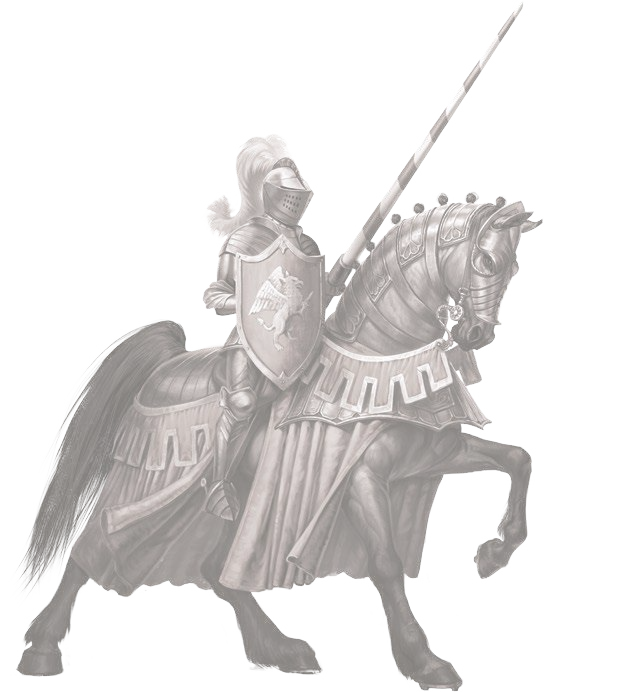
\includegraphics[width=0.6\linewidth]{\art/cavalryman.png}};
\end{tikzpicture}


\addsection{Deckbuilding}{\skills/wisdom.png}

\begin{multicols*}{2}

\subsection*{\hypertarget{Playerdecks}{Player Decks}}
All players have a unique deck which represents their Main Hero's Abilities and Equipment.
Decks may contain Statistic, Ability, Spell, Artifact and the Main Hero's Specialty Cards.

Each player's deck starts with 9 cards, built during the game's set up.
This deck is called your \textbf{Deck of Might \& Magic}. From this point in this rule book this is \textbf{shorthanded} to \textbf{Your Deck}.
\subsection*{General Card Rules}
\begin{enumerate}
  \item Cards can be played \textbf{only on your turn}, or in a \hyperlink{Combat}{Combat} involving your \textbf{Main Hero}.
  \item After a card is used, discard it.
    Each player has their own separate Discard Pile for their own deck.
  \item If Your Deck is empty when you need to draw a card, \textbf{shuffle your Discard Pile} into a new deck to draw from.
  \item Whenever a Hero gains a card for any reason, put it \textbf{directly into your hand} unless otherwise stated.
  \item Whenever you are instructed to \textbf{Search} (X) the Ability, Artifact, or Spell Deck, you may either look at the top (X) cards from the specified deck, take one of them to your hand, and discard the others, \textbf{OR} instead of looking at the top (X) cards, add the top card from that deck's Discard Pile to your hand.
  \item The Ability, Artifact, and Spell Decks each have their own Discard Piles, created during the set up, which help players identify these decks.
    If a deck ever runs out of cards, reshuffle it and discard its top card to form a new Discard Pile.
    Also, whenever one of these Discard Piles is empty, \textbf{refill it} with that deck's top card.
  \item Cards in Your Deck have the following types of effects:
  \begin{itemize}
        \item \textbf{Instant} \includesvg[height=10px]{\svgs/instant.svg} Effects are resolved immediately and can be played out of turn during Combat.
        \item \textbf{Activation} \includesvg[height=10px]{\svgs/activation.svg} Effects must be played when Activating your own Unit in Combat.
        \item \textbf{Map} \includesvg[height=10px]{\svgs/map.svg} Effects cannot be used during Combat.
        \item \textbf{Ongoing} \includesvg[height=10px]{\svgs/ongoing.svg} Effects last until they are used up or until the player who played them starts their next turn (whichever happens first).
        \item \textbf{Permanent} \includesvg[height=10px]{\svgs/permanent.svg} Cards stay in your play area until discarded or replaced.
          \textbf{Players may have only one permanent card at a time}; playing another discards the first.
    \end{itemize}
\end{enumerate}

\clearpage

\subsection*{\hypertarget{Ability}{Ability and Statistic Cards}}

All Ability and Statistic cards have a Basic Effect and a stronger Expert \includesvg[height=10px]{\svgs/expert.svg} Effect, which is shown below the Basic Effect.
Whenever you play an Ability or Statistic card, you must choose which effect you are using.
The number of \includesvg[height=10px]{\svgs/expert.svg} Effects you can use each round is limited by your Main Hero's \hyperlink{Level}{Level}.
Track the number of uses you have in any suitable manner, such as by moving Black Cubes on and off your Hero Card.\par
\bigskip

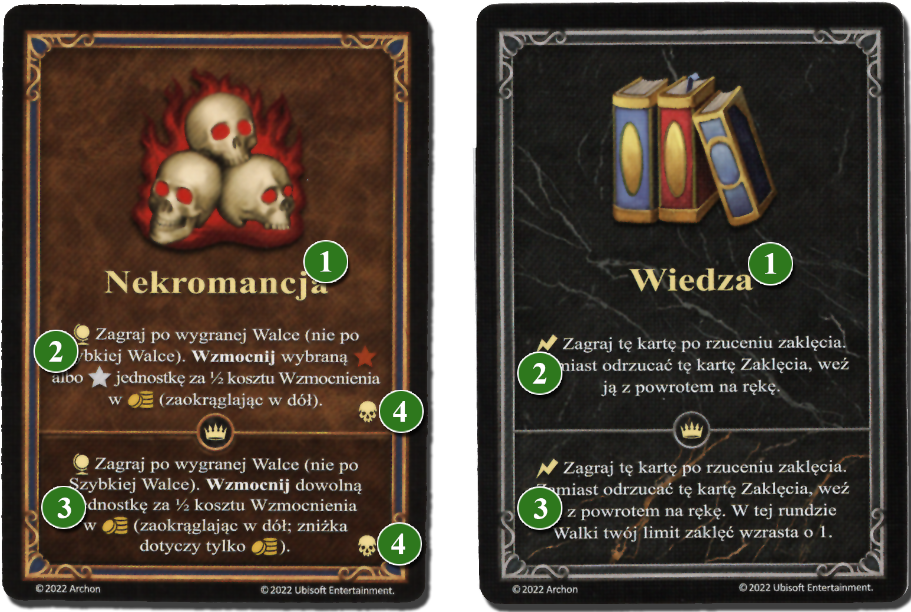
\includegraphics[width=\linewidth]{\cards/ability.png}

\textbf{Important}: Certain cards are limited to the Necropolis Faction \includesvg[height=10px]{\svgs/necro.svg}.
When a non-Necropolis player draws one from the Ability deck, they may either discard it and draw a new card as a replacement or gain it as normal.
Non-Necropolis players \textbf{cannot use} Faction Specific Cards from their hand in any way besides for effects that discard them.

\subsection*{Artifact Cards}
Artifact Cards are divided into 3 levels: Minor, Major, and Relic.
These levels relate to the overall power of the card and may be referenced when resolving certain effects or during Scenario set up.
Otherwise, all Artifact Cards are normally shuffled together regardless of their level.
Artifacts are gained through map exploration.\par
Artifacts can be \hyperlink{Trading}{traded} in Alliance and Cooperative Scenarios.\par
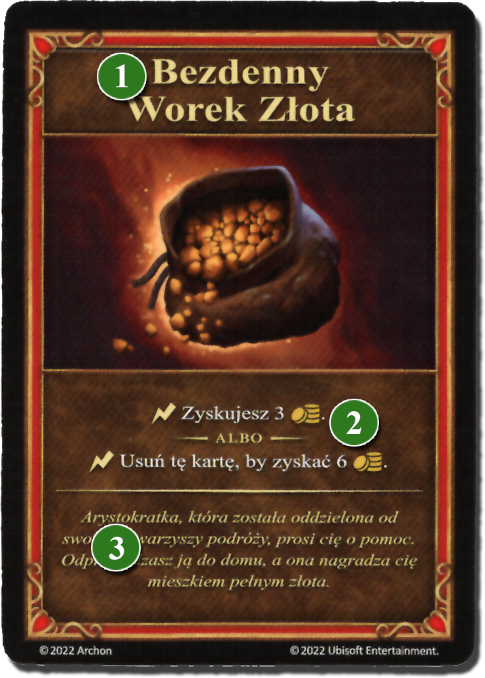
\includegraphics[width=\linewidth]{\cards/artifact.png}

\subsection*{\hypertarget{spells}{Spell Cards}}


Spell Cards have three possible primary effects.
Using the topmost, basic version of the Spell has no additional costs.
To access the other effects, you may \textbf{Empower} a spell by paying the indicated cost (3) to get a more powerful outcome (4).
You may pay this cost by playing other cards for their Empower \includesvg[height=10px]{\svgs/empower.svg} effect before casting the Spell.
All Spell Cards also have an alternative bottom (5) \includesvg[height=10px]{\svgs/empower.svg} effect.\par

\filbreak
\begin{center}
  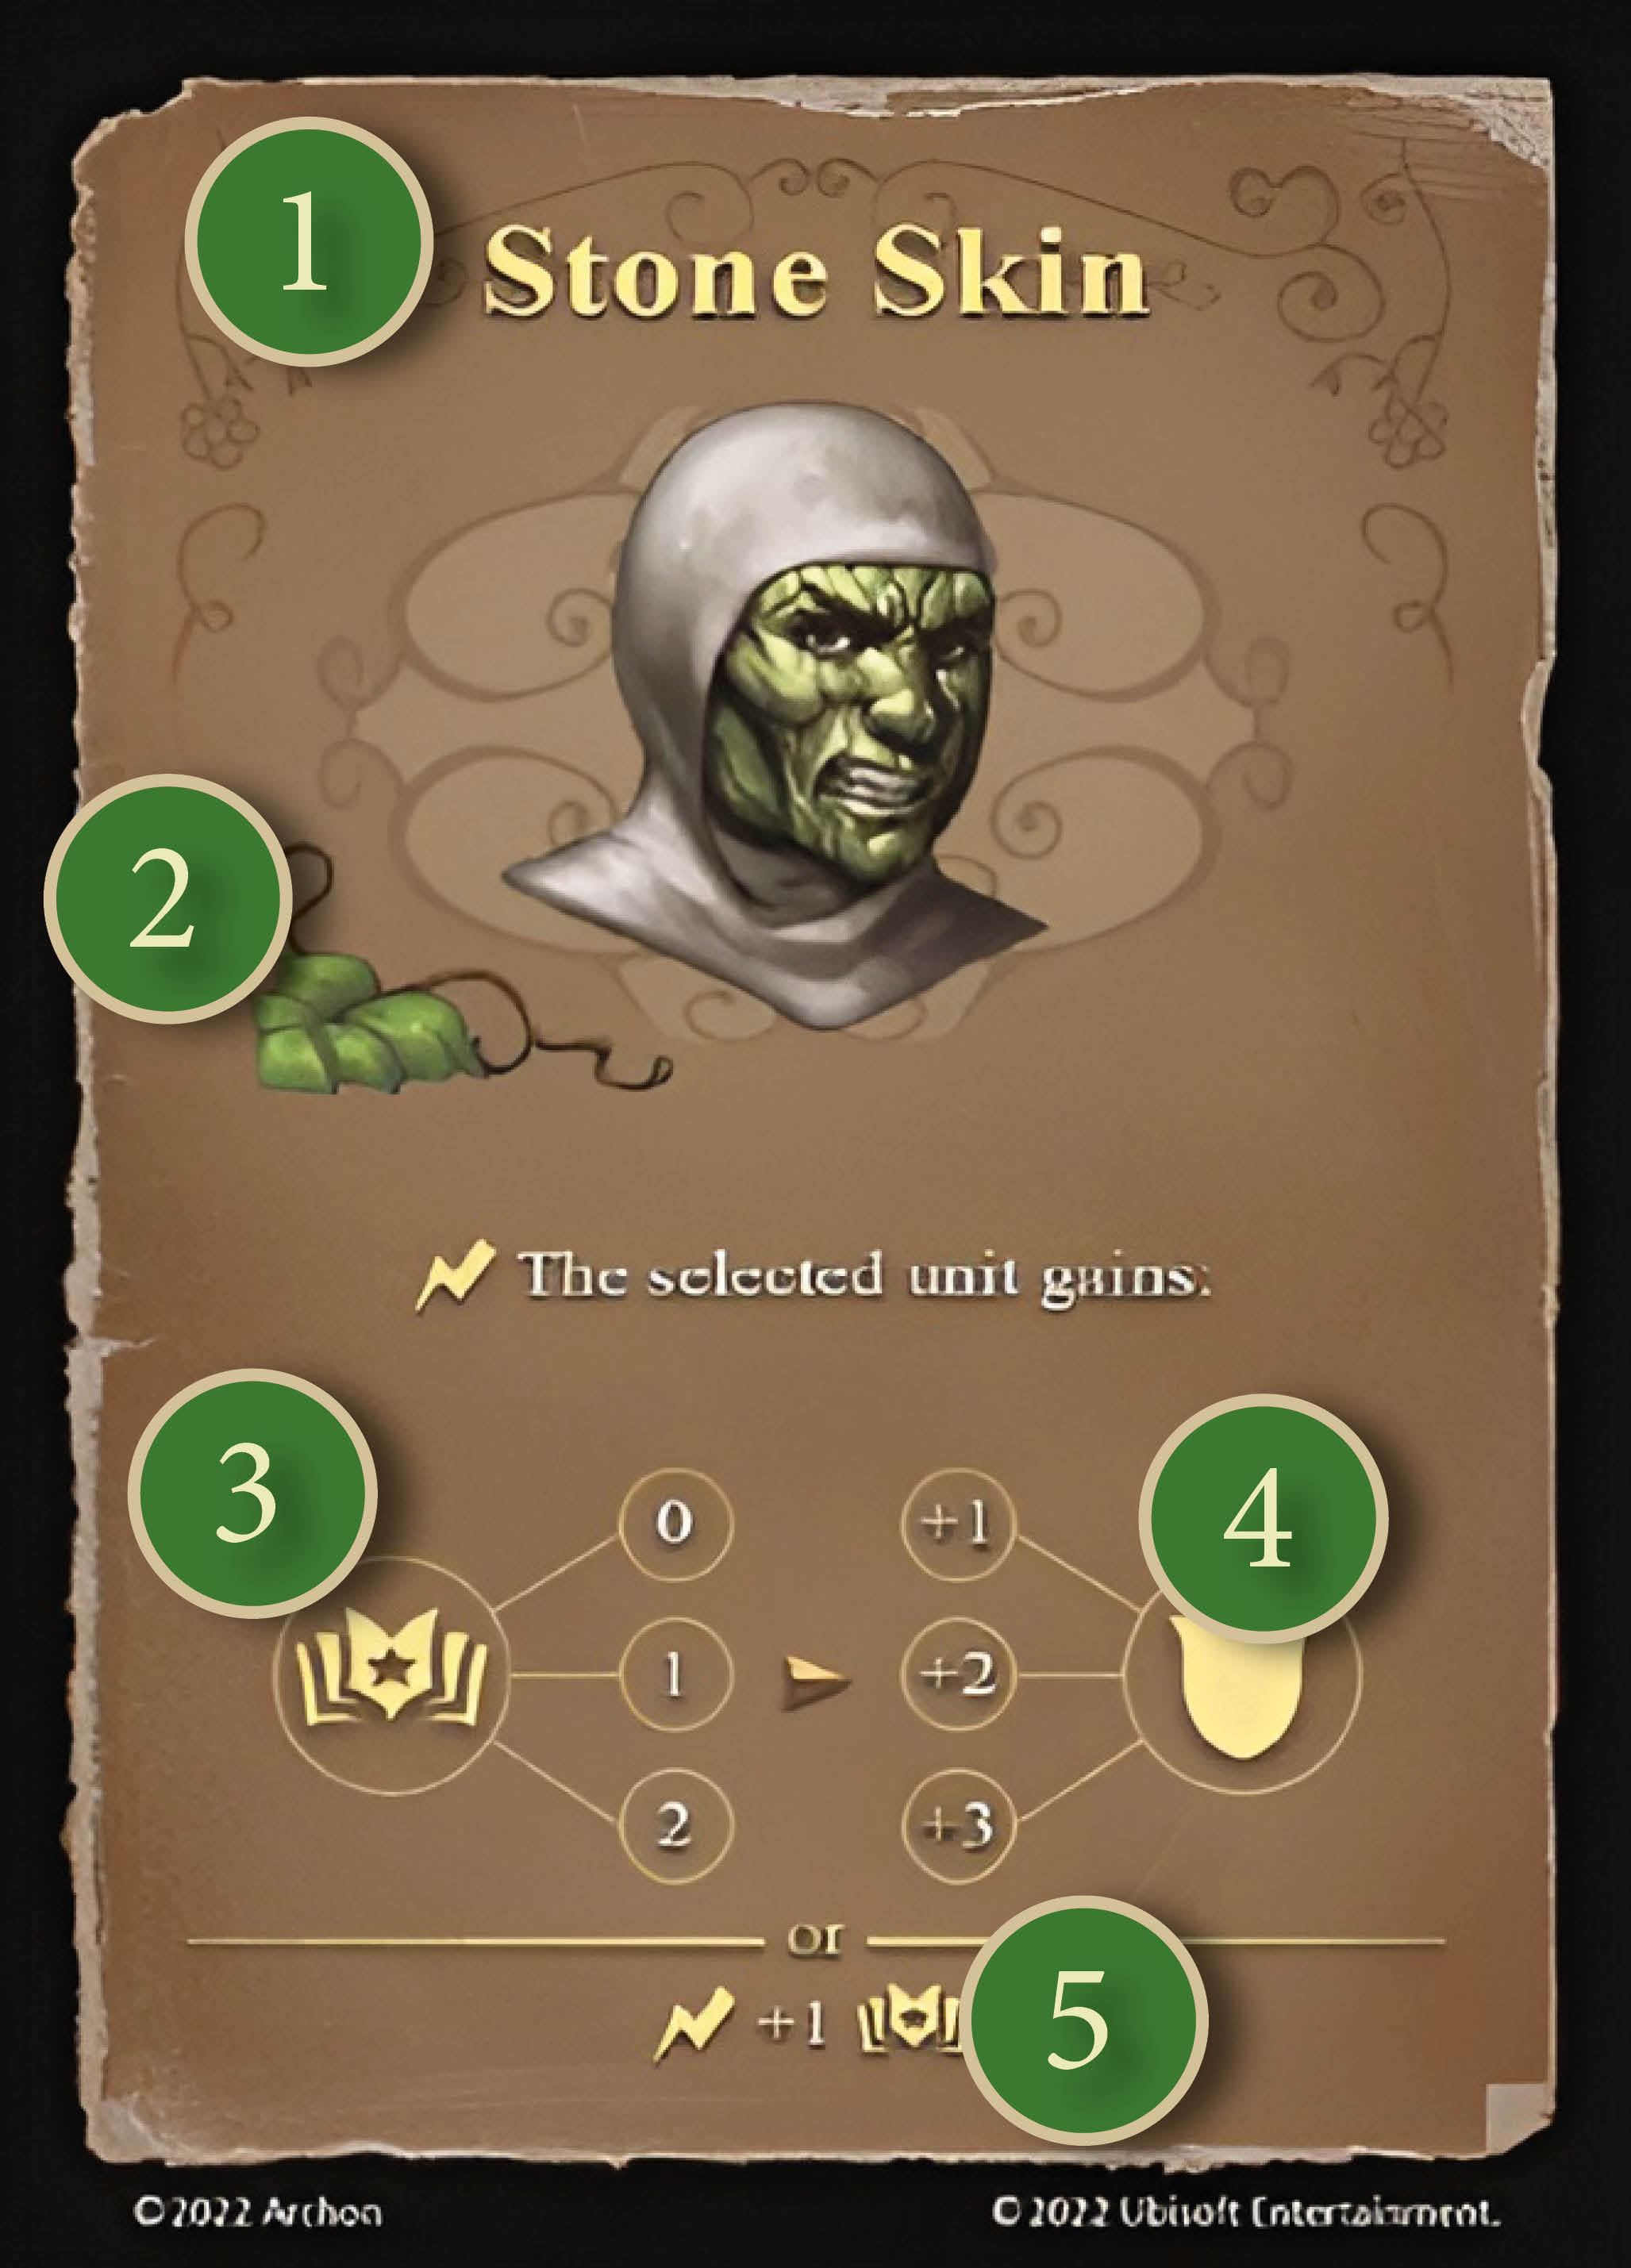
\includegraphics[width=0.6\linewidth]{\cards/spell_example.jpg}\\
  \medskip
  \footnotesize{\textbf{\textit{\textcolor{darkcandyapplered}{Spell Card}}}}
  \scriptsize
  \begin{multicols}{2}
    \begin{itemize}[itemsep=5pt]
      \item[\textbf{1.}] \textbf{Spell Name}
      \item[\textbf{2.}] \textbf{School of Magic}
      \item[\textbf{3.}] \textbf{Cost to Empower}
      \item[\textbf{4.}] \textbf{Spell Effect}
      \item[\textbf{5.}] \textbf{Alternative Effect}
      \item[]
    \end{itemize}
  \end{multicols}
\end{center}

\textbf{Important}: During Combat, \textbf{only one Spell Card} may be played by each player \textbf{per Combat Round}.\par
Spells can be gained by Building the Mage Guild.
When you do, \textbf{Search} (2) the Spell Deck, \textbf{twice}.
If you start a Scenario with the Mage Guild, perform the searching in turn order and shuffle the cards you gained into your deck at the end of the set up.\par
More Spells can be bought by flipping your Spell Book Token and paying the indicated cost on the Mage Guild to \textbf{Search} (2) the Spell Deck.
This cannot be done during the \textbf{same round} as when the Guild is constructed.\par
Spells can be \hyperlink{Trading}{traded} in Alliance and Cooperative Scenarios.

\subsection*{\hypertarget{Specialty}{Hero Specialty Cards}}

Hero Specialty Cards are gained from \hyperlink{Level}{Level ups}.
Each Main Hero has an unique set of them.
While many Specialty Cards have effects which resemble Spell Cards, Specialty Cards are their \textbf{own unique category of card}, which are not affected by effects that do not specify them.

\begin{center}
  \shadowimage[width=0.6\linewidth]{\cards/specialty.jpg}\\
  \medskip
  \scriptsize\textit{A level 4 Specialty Card, belonging to Catherine the knight.}
\end{center}

\vspace*{\fill}

\begin{center}
  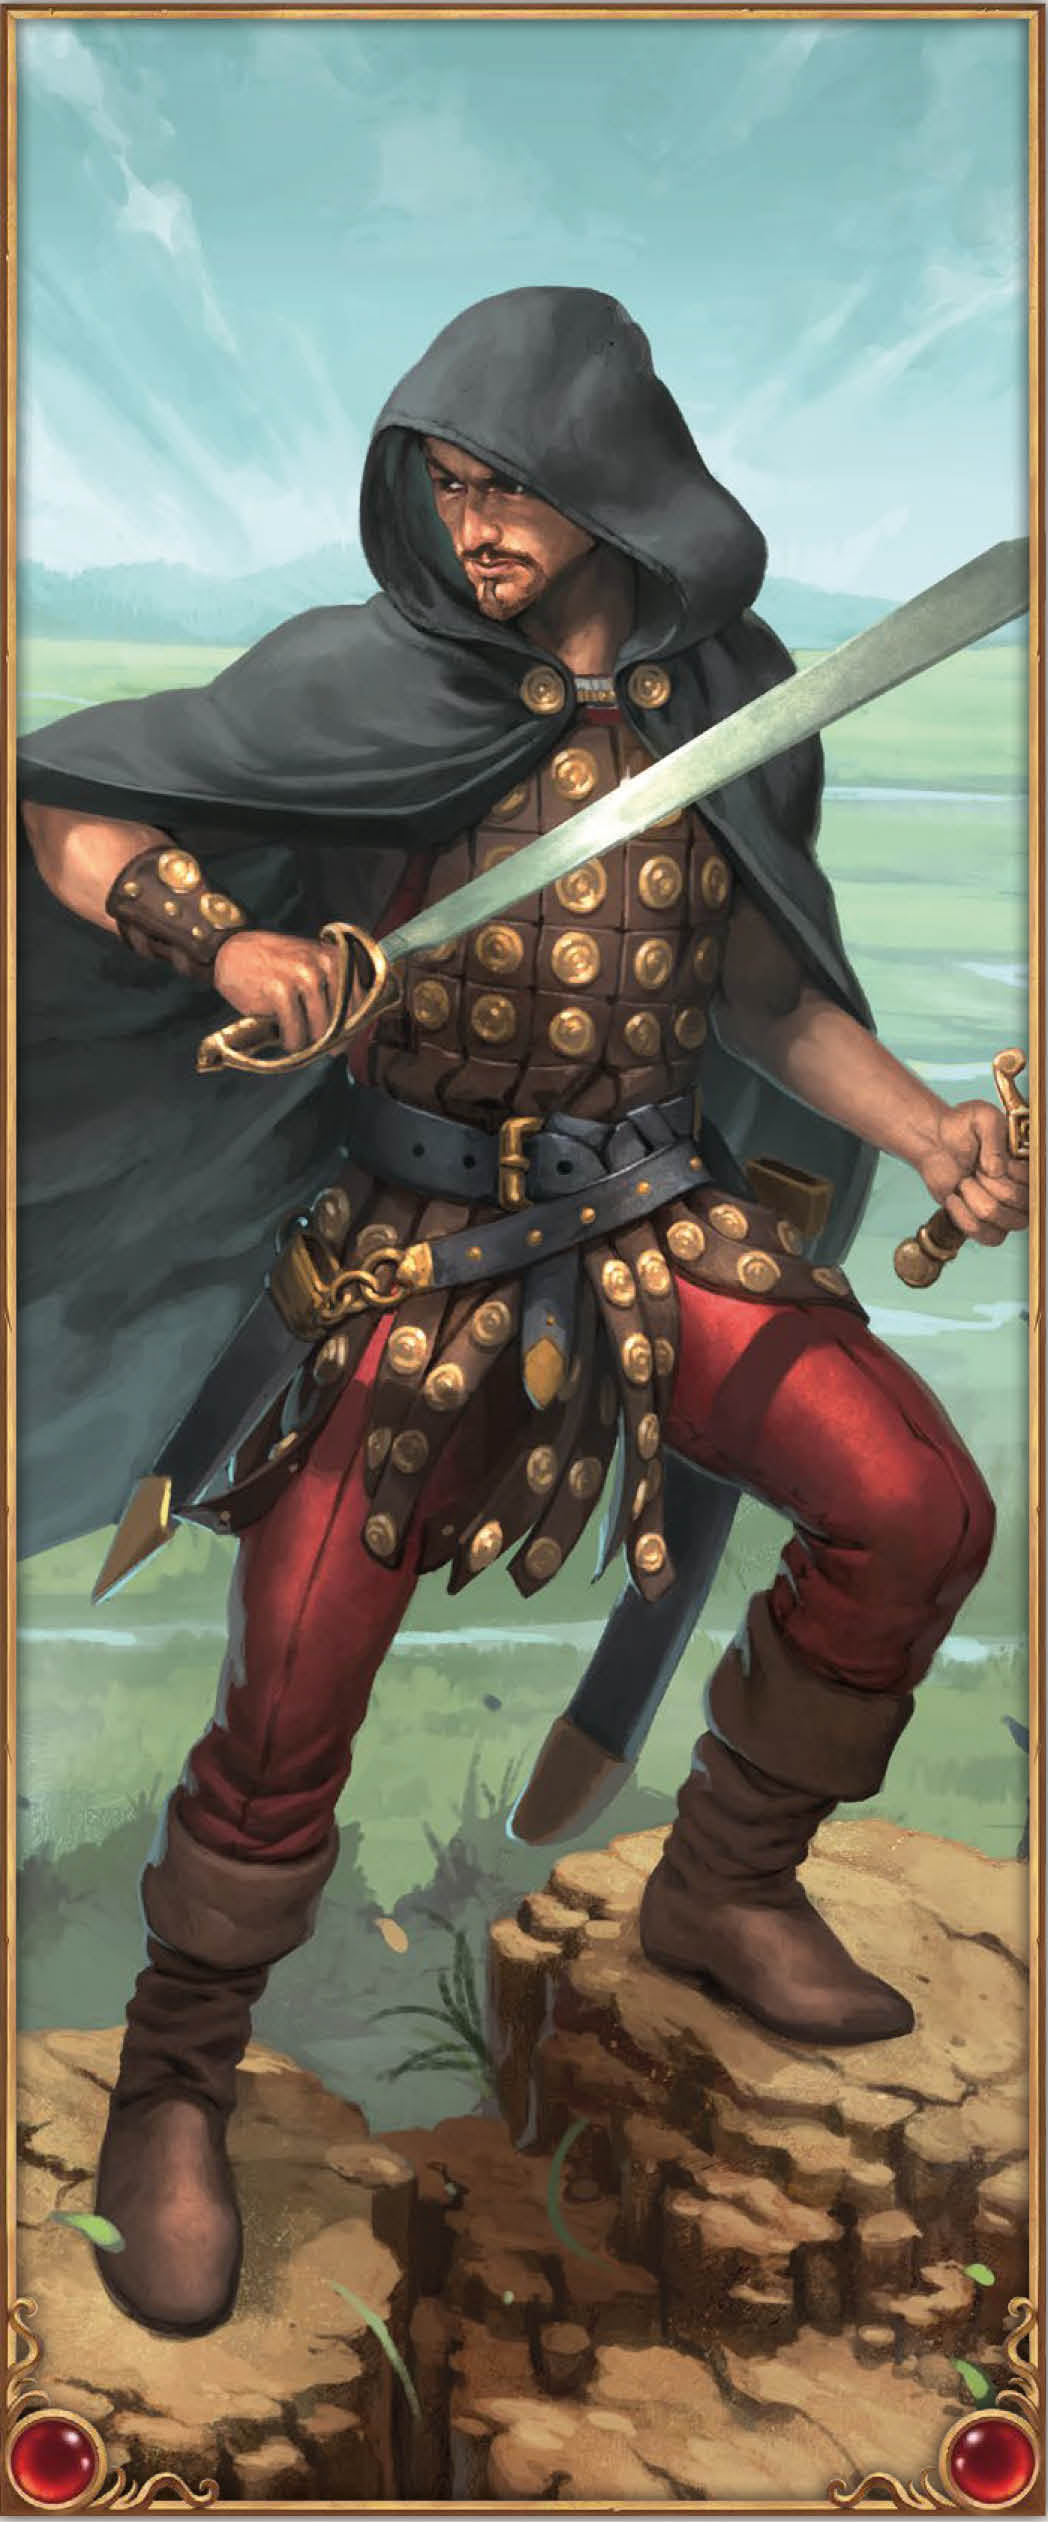
\includegraphics[width=0.8\linewidth]{\art/rogue.jpg}
\end{center}

\end{multicols*}

\clearpage

\begin{multicols}{2}

\textit{Deemer the Warlock has built a Mage Guild during the previous Game Round, enabling him to now use his Spell Book Token to purchase additional spells.
He spends the token and pays the cost indicated on his Town Board, allowing him to \textbf{Search (2)} the Spell Deck.}\par
\textit{He now has the choice of either gaining the top card of the Spell Card discard pile, or drawing the top two cards of the Spell Deck and gaining one of them.
He is not interested in gaining the Spell Curse, which is on top of the discard pile, and instead decides to draw  two cards – a Magic Arrow and a Fireball.
He decides to keep the Fireball, placing it into his hand and discarding the Magic Arrow into the Spell Discard Pile.}

\end{multicols}

% !TeX spellcheck = en_US
\addsection{Resources}{\skills/estates.png}

\begin{multicols}{2}

\hypertarget{Resources}{There} are three types of Resources in the game: Gold \includesvg[height=10px]{\svgs/gold.svg}, Building Materials \includesvg[height=10px]{\svgs/building_materials.svg}, and Valuables \includesvg[height=10px]{\svgs/valuablegreater.svg}.
Resources are spent during the game to expand your \hyperlink{Town}{Town}, to Recruit \hyperlink{Units}{Units}, and to purchase \hyperlink{spells}{Spells}.
You can gain Resources from the \hyperlink{Mines}{Settlements and Mines} that you have \hyperlink{Categories}{Flagged}, but also by playing Cards and rolling Resource Dice \includesvg[height=10px]{\svgs/resource_die.svg}.
Whenever a player's Resource Production is increased or decreased, move that Resource's cube on its production track the appropriate number of spaces.\par
\begin{multicols}{3}
  \centering
  \vspace*{\fill}
  
\includegraphics[width=0.8\linewidth]{\images/gold.png}
  \footnotesize\textcolor{darkcandyapplered}{\textit{\textbf{Gold \phantom{Materials}}}}
  \columnbreak
  \vspace*{\fill}
  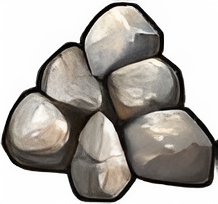
\includegraphics[width=0.8\linewidth]{\images/building_materials.png}
  \footnotesize\textcolor{darkcandyapplered}{\textit{\textbf{Building Materials}}}
  \columnbreak
  \vspace*{\fill}
  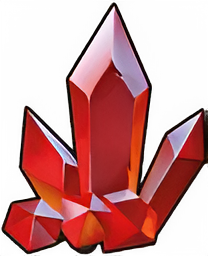
\includegraphics[width=0.8\linewidth]{\images/valuables.png}
  \footnotesize\textcolor{darkcandyapplered}{\textit{\textbf{Valuables \phantom{Materials}}}}
\end{multicols}
Players start each Scenario with the number of Resources indicated in that Scenario’s setup.
Resources can also be \hyperlink{Trading}{traded}.
There's no limit to the amount of Resources you can have.

\vspace*{\fill}

\columnbreak

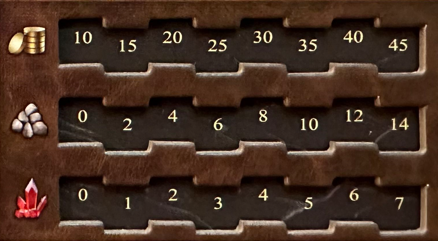
\includegraphics[width=\linewidth]{\tables/resource_board.png}
\smallskip
\centering\footnotesize\textcolor{darkcandyapplered}{\textbf{\textit{Resource Production Tracker}}}
\bigskip

Possible Resource Die \includesvg[height=10px]{\svgs/resource_die.svg} results:
\medskip
\begin{itemize}
  \setlength\itemsep{8pt}
  \item \includesvg[height=15px]{\svgs/2_building_materials.svg} - 2 x Building Materials
  \item \includesvg[height=15px]{\svgs/4_building_materials.svg} - 4 x Building Materials
  \item \includesvg[height=15px]{\svgs/1_valuables.svg} - 1 x Valuables
  \item \includesvg[height=15px]{\svgs/2_valuables.svg} - 2 x Valuables
  \item \includesvg[height=15px]{\svgs/3_gold.svg} 3 x Gold
  \item \includesvg[height=15px]{\svgs/6_gold.svg} 6 x Gold
\end{itemize}

\end{multicols}

\vspace*{\fill}

\begin{scaledfigure}[blanker]
  \centering
  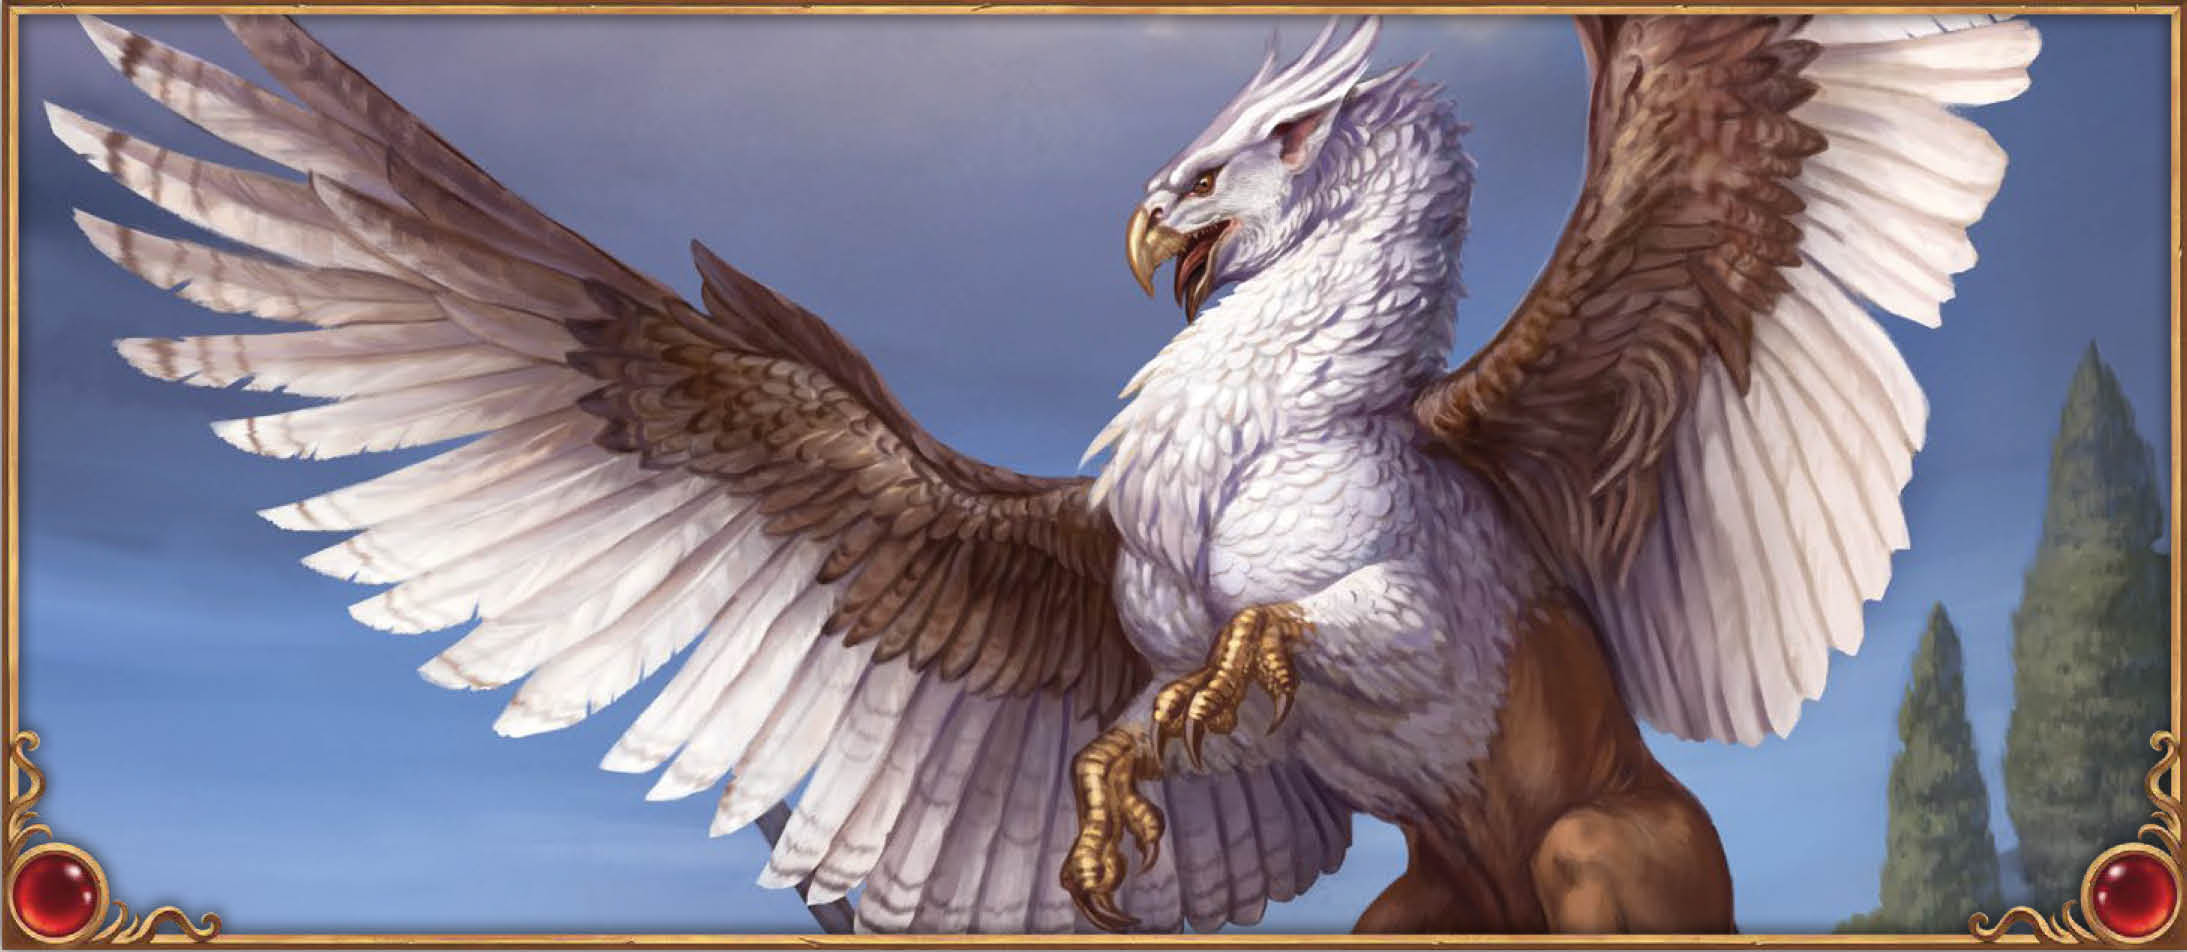
\includegraphics[width=\linewidth, height=\myspace, keepaspectratio]{\art/griffin.jpg}
\end{scaledfigure}


% !TeX spellcheck = en_US
\addsection{Town}{\skills/artillery.png}

\begin{multicols*}{2}

\hypertarget{Town}{Each}\index{Town} Faction has their own Town, which is located in the center of their Starting Tile.
The Town is your most important location, as many Scenarios \hyperlink{End}{may end} if it's \hyperlink{Categories}{Flagged} by an enemy Hero.\par
The contents of your Town and overall Faction status are represented by the Town Board.
It shows your currently built Buildings, Resource costs for future Buildings, your Resource incomes and status of Town Action Tokens.\par
All Factions are able to Build the following Buildings\index{Buildings} in their Town:
\begin{itemize}
  \item \textbf{City Hall} – Provides Resource income or a Faction-Specific Ability.
  \item \textbf{Citadel} – Allows you to Reinforce Units when using the Population Token.
Also \hyperlink{Walls}{protects your Town} when it is attacked.
  \item \textbf{Unit Dwellings} – Allows you to Recruit Units.
Dwellings have three Levels that unlock new Units, but which must be Built in the following order:\includesvg[height=10px]{\svgs/bronze.svg}\includesvg[height=10px]{\svgs/silver.svg}\includesvg[height=10px]{\svgs/Golden.svg}
  \item \textbf{Mage Guild}\index{Mage Guild} - gives you \hyperlink{spells}{Spells}.
  \item \textbf{Faction Building} - a Faction-Specific Building with a unique effect.
\end{itemize}
\textbf{A single Building} may be Built each Round by using the Build Token\index{Build Token}.
When you build a Building, pay its cost in Resources, flip the Build Token to its inactive side, and place the new Building’s Cardboard Piece into its proper slot on the Town Board.
If the Building has any immediate effects upon Building it, resolve them now.\par
Built Buildings are always represented by a symbol within a circle.
Buildings that can be built in the future are represented by a rectangle that contains the Building's cost in Resources.
Many Building Tiles are double-sided, and may later be upgraded and flipped to represent two different buildings at the same time. Such upgrades must be Built in order.\par
If a Town or Settlement is attacked by an enemy hero and your Hero is not also on that Field, you may immediately \textbf{pay 8 Gold} to fight a defending Combat \textbf{using only your Units}.
You cannot use your Deck during that Combat as your Main Hero is not present.
Paying this Gold represents the cost of transporting the army there.\par
When you \hyperlink{Categories}{Flag} a Town, take \hyperlink{End}{a Faction Cube} from its previous owner.

\vspace*{\fill}

\begin{center}
  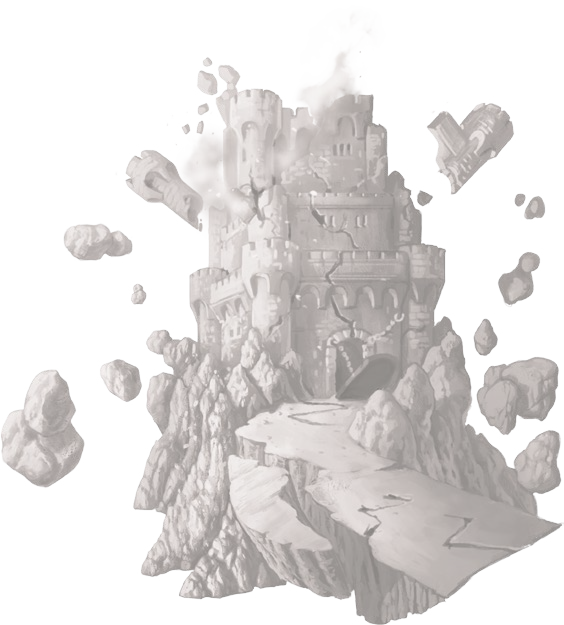
\includegraphics[width=\linewidth]{\art/earthquake.png}
\end{center}

\vspace*{\fill}

\end{multicols*}


% !TeX spellcheck = en_US
\addsection{Map Elements}{\skills/logistics.png}

\begin{multicols*}{2}
Each Scenario is built using four types of Map Tiles.
Players start on their Faction-Specific Starting (I) Tile.
Other tiles may be placed and discovered as described on the next page.
During the game's setup, all face-down tiles should be selected randomly from the pool of possible Tiles as described by the Scenario and shuffled, keeping them face-down.\par
The \textbf{roman numeral} on each tile describes the overall \textbf{difficulty of Neutral Units} on that tile, as well as the number of rewards players can expect to find on that Tile.
Starting (I) Tiles are the easiest while Center (VI–VII) Tiles are the most difficult.\par

\vfill
\begin{center}
  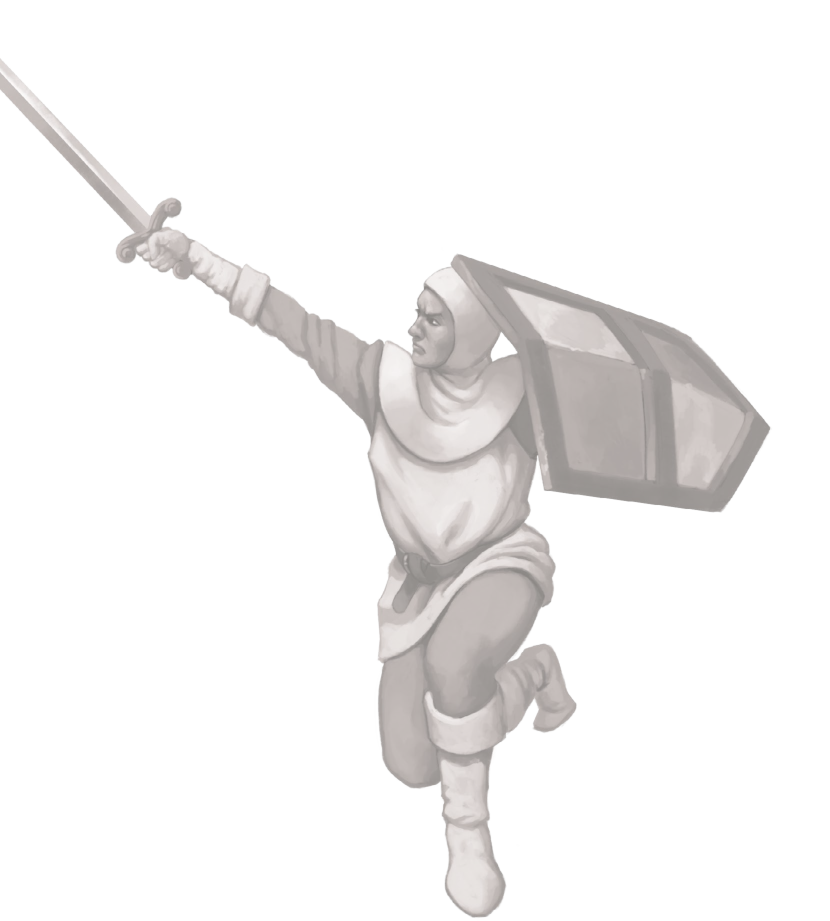
\includegraphics[width=0.7\linewidth]{\art/counterstrike.png}
\end{center}
\vfill

\subsection*{Map Tile Anatomy\index{Map Tile}}
Each Map Tile is divided into 7 separate \textbf{Fields} that your Heroes can \textbf{Visit}.
When your Hero moves to a Field, they must immediately Visit it, or
first start a \hyperlink{Combat}{Combat} against the enemies guarding it before Visiting.
Empty Fields\index{Empty Field} do nothing when Visited.
Solid yellow lines on a Field's edge cannot be passed through.
\hyperlink{Difficulty}{Roman numerals} written on a Field indicate that the Field is guarded by Neutral enemies that must be fought to Visit it.\par
\columnbreak
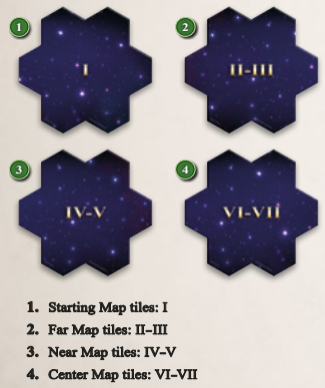
\includegraphics[width=\linewidth]{\images/maptiles.png}
\begin{itemize}
  \footnotesize
  \item[\textbf{1.}] Starting Map Tiles: I
  \item[\textbf{2.}] Far Map Tiles: II-II
  \item[\textbf{3.}] Near Map Tiles: IV-V
  \item[\textbf{4.}] Center Map Tiles: VI-VII
\end{itemize}

\vfill
\begin{center}
  \begin{scriptsize}
  \begin{tikzpicture}
    \draw (0, 0) node[inner sep=0] {\makebox[\linewidth][c]{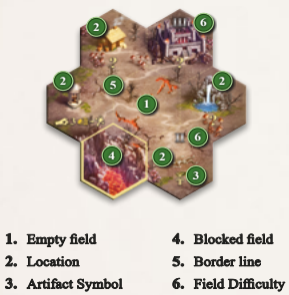
\includegraphics[width=0.75\linewidth]{\images/fields.png}}};
    \draw (0, -0.3) node {\encircle{\phantom{.}1\phantom{.}}};
    \draw (-1.9, 0) node {\encircle{\phantom{.}2\phantom{.}}};
    \draw (2.3, 0) node {\encircle{\phantom{.}2\phantom{.}}};
    \draw (-1.4, 1.7) node {\encircle{\phantom{.}2\phantom{.}}};
    \draw (0.6, -1.9) node {\encircle{\phantom{.}2\phantom{.}}};
    \draw (0.5, 1.7) node {\encircle{\phantom{.}2\phantom{.}}};
    \draw (1.4, -2.2) node {\encircle{\phantom{.}3\phantom{.}}};
    \draw (1.4, 2.5) node {\encircle{\phantom{.}4\phantom{.}}};
    \draw (1.4, -1) node {\encircle{\phantom{.}4\phantom{.}}};
    \draw (-1, 0.5) node {\encircle{\phantom{.}5\phantom{.}}};
    \draw (-1.1, -1.1) node {\encircle{\phantom{.}6\phantom{.}}};
    \draw (-1.4, -1.7) node {\encircle{\phantom{.}7\phantom{.}}};
  \end{tikzpicture}
  \end{scriptsize}
\end{center}

\begin{itemize}
  \footnotesize
  \begin{multicols}{2}
    \item[\textbf{1.}] Empty Field
    \item[\textbf{2.}] Location
    \item[\textbf{3.}] Artifact Symbol
    \item[\textbf{4.}] Field Difficulty
    \item[\textbf{5.}] Border line
    \item[\textbf{6.}] Blocked Field
    \item[\textbf{7.}] Tile name like \\{} \texttt{F2} or \texttt{\#N3}
  \end{multicols}
\end{itemize}

\note{3}{
  Blocked Field cannot be entered, but can be exited.
}
\end{multicols*}

\clearpage

\begin{multicols}{2}

\subsection*{\hypertarget{Categories}{Location Categories}}
Visiting Fields provides Heroes with benefits, such as gaining Resources or Cards (see \hyperlink{All Map Locations}{All Map Locations}).
There are three categories of Fields:
\begin{itemize}
  \item \textbf{Visitable} – Once you Visit this field, place a Black Cube on it.
    Treat it as an Empty Field as long as it has a Black Cube.
  \item \textbf{Flaggable} – These Fields can be captured by players and provide passive benefits.
    When you Visit one, place your Faction Cube on it.
    Enemy Heroes who Visit your Flagged Fields will replace your Cube with theirs to \textbf{steal} the Field’s effects.
    Allied Heroes treat Flagged Fields \textbf{as if they were empty}.
  \item \textbf{Revisitable} – You can Visit this Field multiple times.
    Do not place any Cubes when you Visit it.
    You may pay 1 MP to Visit this Field again.
\end{itemize}

\subsection*{\hypertarget{Placing}{Placing and Discovering New Tiles}}\index{Discovering Tiles}
Heroes may spend 1 MP to either reveal an adjacent face-down Tile, or to place a Far (II–III) Map Tile from their own supply of Tiles.
All face-down Tiles should be kept \textbf{hidden from all players} until they are about to be placed or revealed.
New tiles must be placed adjacent to the Hero who spends the MP, and connected to at least two other existing Tiles.
New Tiles must also be positioned so that there is a valid path that eventually connects them with all other Tiles.
You may always rotate Map Tiles when placing or revealing them.

\medskip
\note{6}{
  When you Visit a Visitable field, \textbf{you must} place a black cube on that Field even if you cannot or choose not to use that Field's effects.
}

\end{multicols}

\begin{figure*}[!hb]
  \centering
  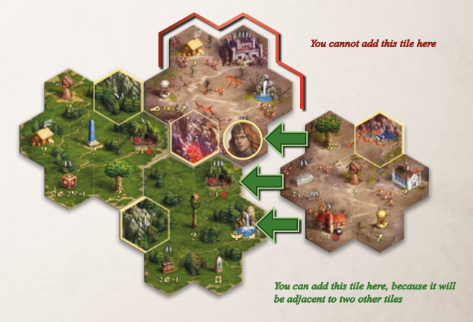
\includegraphics[width=\textwidth]{\images/placement.png}
  \begin{tikzpicture}[overlay]
    \node at (5, 10) {\footnotesize{\textbf{\textit{\textcolor{darkcandyapplered}{You cannot add this tile here}}}}};
    \node at (5, 1.4) {\footnotesize{\textbf{\textit{\textcolor{cadmiumgreen}{You can add this tile here, because it will}}}}};
    \node at (3.9, 1) {\footnotesize{\textbf{\textit{\textcolor{cadmiumgreen}{be adjacent to two other tiles}}}}};
  \end{tikzpicture}
\end{figure*}

\clearpage

\subsection*{Example Turn}

\begin{multicols*}{2}

\textit{Alice wants to capture an adjacent \hyperlink{Mines}{Mine} by Flagging it with her Main Hero, Sandro the Necromancer.
    She spends 1 MP to move onto the Mine, which begins \hyperlink{Combat}{Combat} against Neutral Units, since the Field has a \hyperlink{Difficulty}{Difficulty Rating} and has not been previously Flagged by any player.}\par

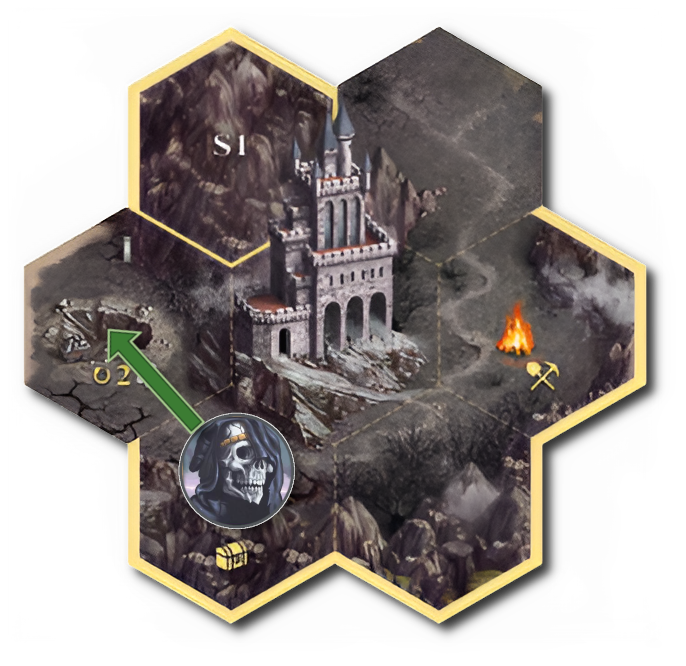
\includegraphics[width=1.1\linewidth]{\examples/sandro_takes_mine.png}

\textit{The Mine turns out to be guarded by Troglodytes, which have 3 HP \includesvg[height=0.8\baselineskip]{\svgs/health_points.svg}.
Alice's current hand consists of a Power Card, a Lightning Bolt, Haste, and a Town Portal.
During the Combat, she casts the Lightning Bolt, and Empowers \includesvg[height=0.8\baselineskip]{\svgs/empower.svg} it with Haste's alternative (bottom) effect, which makes the Lightning Bolt deal 3 damage \includesvg[height=0.8\baselineskip]{\svgs/damage.svg}, killing the Troglodytes and winning the Combat.}

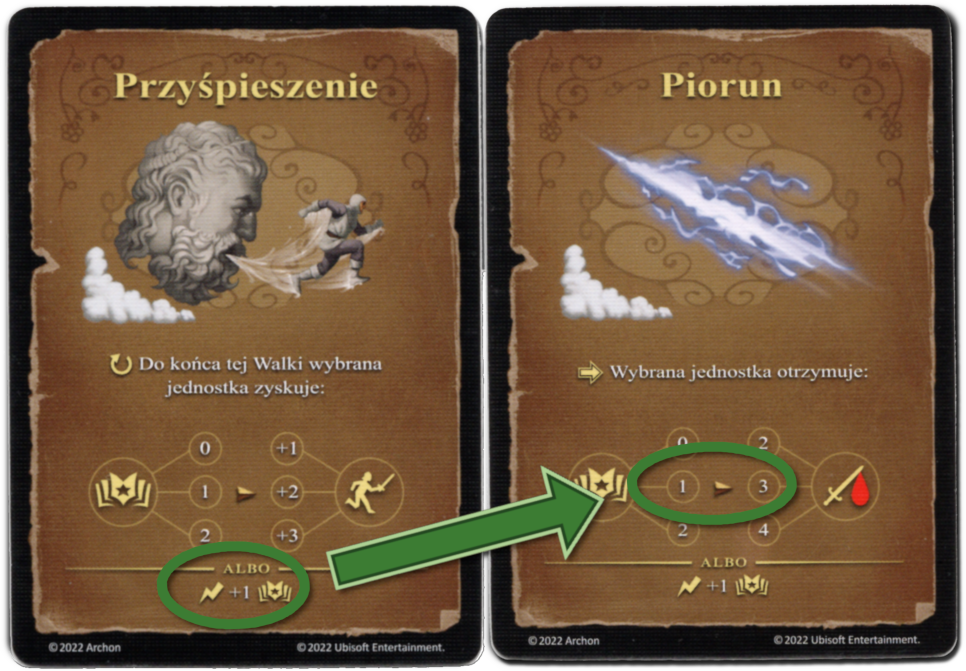
\includegraphics[width=\linewidth]{\examples/sandro_empowering_lightning_bolt.png}

\textit{The Combat lasted for only one Round, so Alice would not have been able to cast both Lightning Bolt and Haste, since players are limited to playing only one Spell Card per Combat Round.}\par


\textit{Alice now Flags the Mine by placing one of her Faction Cubes on it.
    Flagging this particular Mine increases her Building Materials \includesvg[height=0.8\baselineskip]{\svgs/building_materials.svg} production by 2, and she also immediately gains the Mine's production value of 2 \includesvg[height=0.8\baselineskip]{\svgs/building_materials.svg} as she was the first player to Flag it.}\par
\textit{Afterwards, Alice wants to go back to defend a previously Flagged Settlement by casting the Town Portal still left in her hand.
    Her Hero is Level 2, so she can empower it with the Power Card's Expert Effect \includesvg[height=0.8\baselineskip]{\svgs/expert.svg}, which grants her an additional Movement Point after casting it.
}

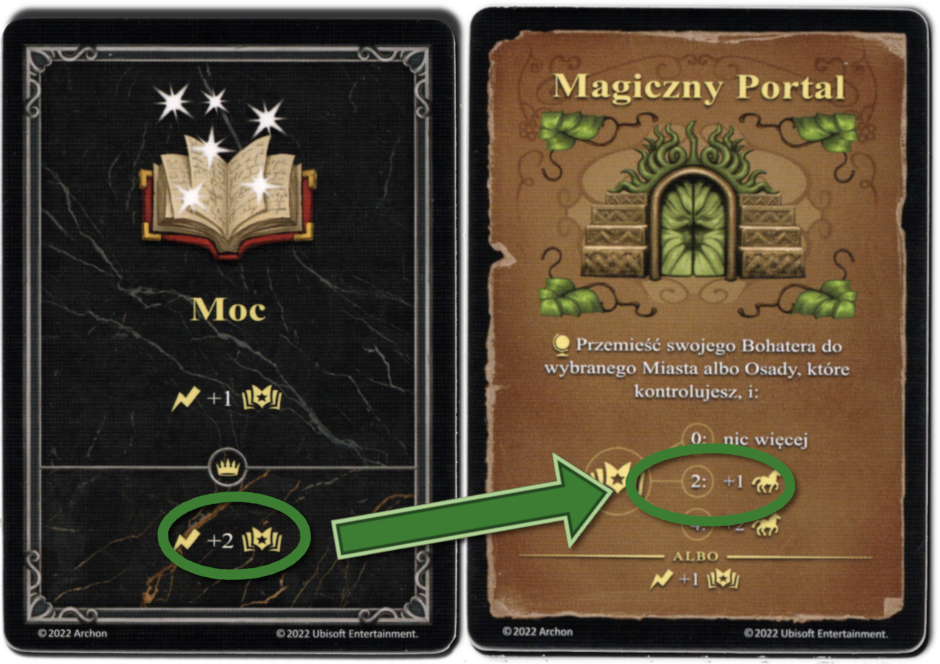
\includegraphics[width=\linewidth]{\examples/sandro_empowering_town_portal.png}

\vfill
\hspace{2em}
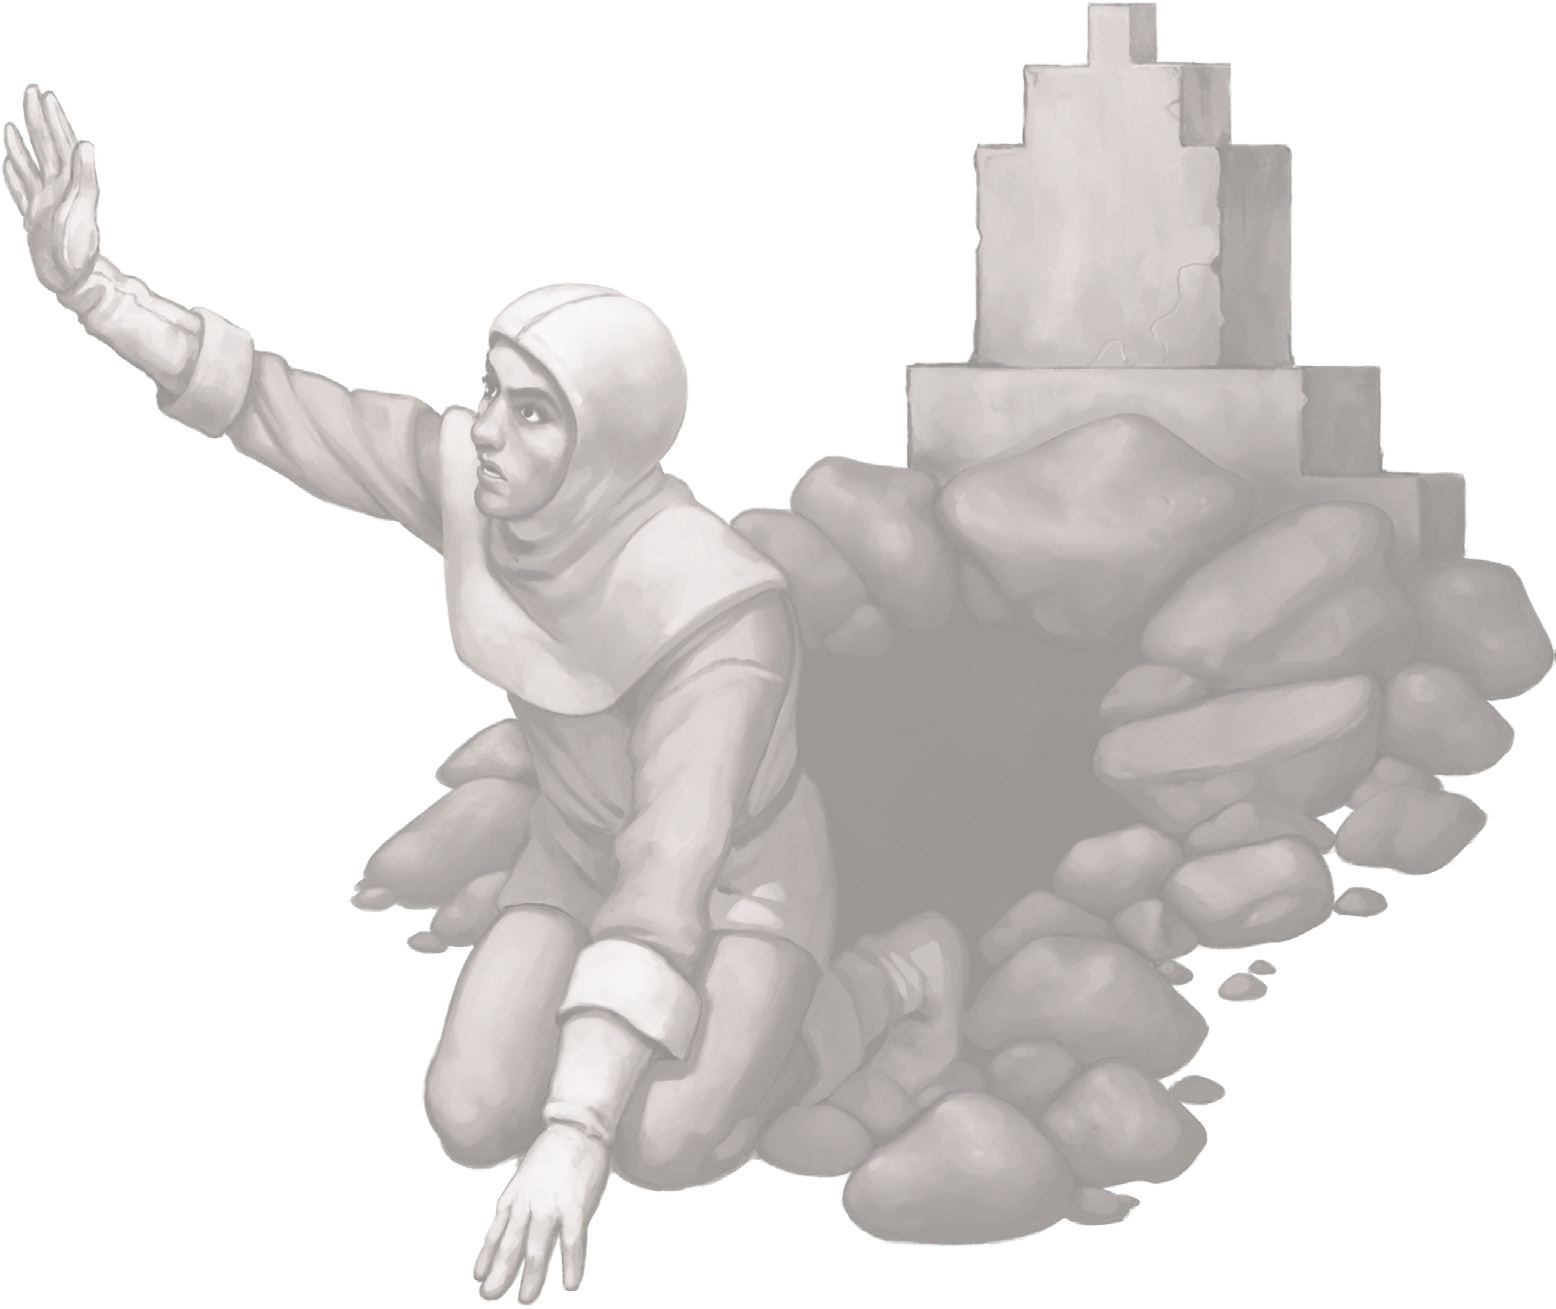
\includegraphics[width=\linewidth]{\art/resurrection.png}
\end{multicols*}


% !TeX spellcheck = en_US
\addsection{Units}{\skills/leadership.png}

\begin{multicols*}{2}

\hypertarget{Units}{In}\index{Units} addition to their Hero and its associated deck, players also have \textbf{a deck of Unit Cards} which represent the armies moving with their Heroes.
Every Faction has access to \textbf{7 different Units}, each with unique stats and abilities.
Units are necessary for winning Combat and fulfilling Scenario goals.
Each Scenario's setup instructions indicate which Unit Cards should be included in your initial Unit Deck.
Your current Unit Deck should be kept near the Town Board, clearly separated from the rest of your Faction's Units.\par
Each Faction Unit is double-sided, with a weaker “Few” side, and a stronger “Pack” side.
“Few” units may be upgraded to “Packs” by \textbf{Reinforcing} them, while taking damage in Combat can subsequently reduce a Unit back to its “Few” side.
Units should be always kept on their correct side when moved around or inspected.\par
A player's Unit Deck may have any number of Units, but \textbf{only up to 5 Units} can be selected to fight during \hyperlink{Combatsetup}{Combat Setup}.
If a unit is defeated in Combat, \textbf{discard it} from your Unit Deck.\par
Units may be Recruited and Reinforced by flipping the Population Token and paying the Unit's Recruitment \includesvg[height=10px]{\svgs/pay.svg} or Reinforcement \includesvg[height=10px]{\svgs/reinforce.svg} cost.
When you do so, you can instantly Recruit and Reinforce \textbf{any number} of times, provided you have enough Resources and the prerequisite Buildings to do so.\par

\textbf{Recruiting} a unit requires that your Town has a Dwelling of that Unit's Level (\includesvg[height=10px]{\svgs/bronze.svg}\includesvg[height=10px]{\svgs/silver.svg} \includesvg[height=10px]{\svgs/golden.svg}).
\textbf{Reinforcing} requires that your Town has a Citadel in addition to a Dwelling of that Unit's Level.
If all Units in your Unit Deck are defeated, \textbf{immediately} replace your Unit Deck with the starting Units of the Scenario. Defeated Faction Units can always be re-Recruited with another use of the Population Token.\par

\note{6}{Any effects which allow you to Reinforce outside of using the Population Token \textbf{do not} require a Citadel or any Dwellings.}\par
\bigskip

\begin{center}
  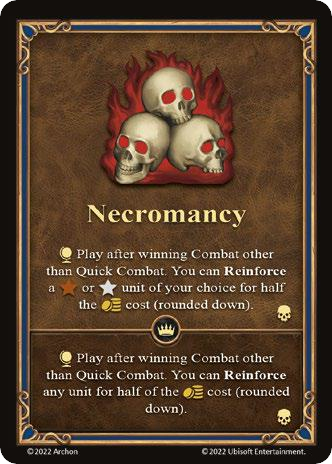
\includegraphics[width=0.6\linewidth]{\cards/necromancy_card.png}\par
  \footnotesize\textit{
    Cards such as Necromancy allow you to Reinforce outside of using the Population Token.
    This does not require owning any of the prerequisite buildings for Reinforcing nor flipping your Population Token.
  }
  \vfill
  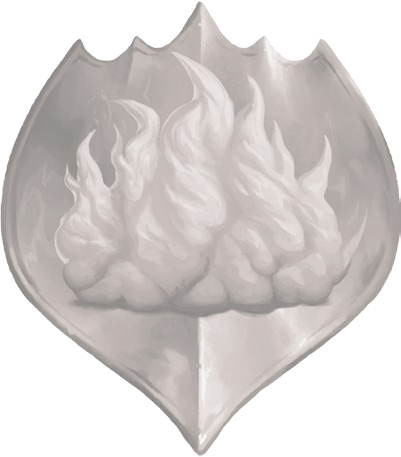
\includegraphics[width=0.6\linewidth]{\art/fire_shield.png}
\end{center}

\clearpage

\end{multicols*}
\begin{multicols}{2}
\subsection*{Unit Card Anatomy}

\vspace{0pt}

\includesvg[height=30px]{\svgs/attack.svg}\textbf{Attack} – The amount of damage this Unit deals when it attacks.
Attacks are always reduced by the defending unit's Defense.
Attacks may be modified by various effects such as the attack die and statistic cards.\par
\includesvg[height=30px]{\svgs/defense.svg}\textbf{Defense} - The amount by which the Unit reduces the attack damage it receives.
Does not apply to damage received from Spells or other non-attack effects.
Defense may be modified by various effects such as Statistic Cards.\par
\includesvg[height=30px]{\svgs/health_points.svg}\textbf{\hypertarget{HP}{HP}} - The maximum amount of damage a Unit can sustain before it is defeated.
”Few” Units are discarded from Combat and its owner's Unit Deck when defeated.
”Pack” Units are turned back to ”Few” units, with any excess damage placed on its ”Few” side.
After Combat, all damage is healed from all Units.
Units retain their ”Few” or ”Pack” status between Combats.\par
\includesvg[height=30px]{\svgs/initiative.svg}{\hypertarget{Initiative}{\textbf{Initiative}}} - Determines when the Unit Activates during Combat.
Units with a higher Initiative Activate first.
In case of a tie, the \hyperlink{Combatterminology}{attacking} side's Unit should always Activate first.
If there are multiple ties on one side, the player who controls those Units selects which Unit to Activate next.
If there are multiple ties on both sides (for instance two attackers and two defenders with the same Initiative), alternate between the attackers and defenders starting with the attacker.\par
\bigskip

\begin{scaledfigure}[blanker]
  \centering
  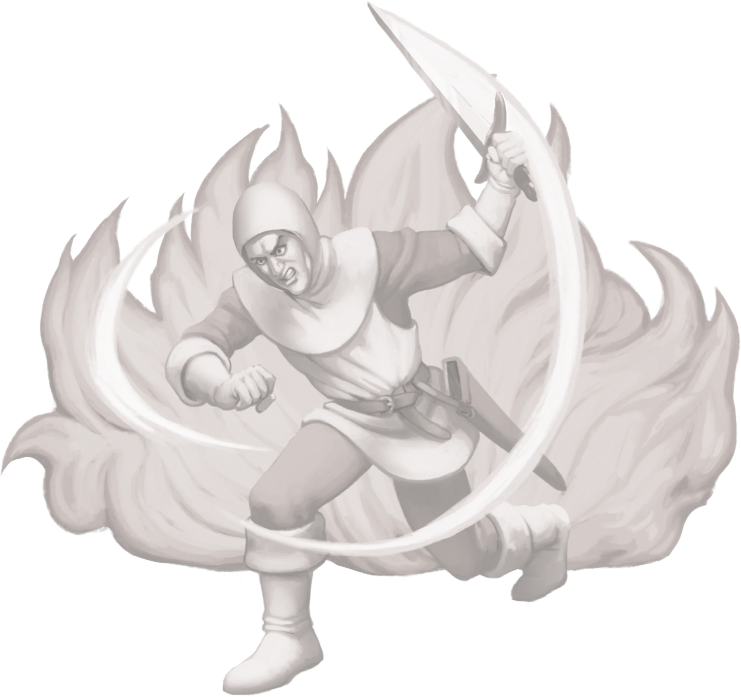
\includegraphics[width=0.5\linewidth, height=\myspace, keepaspectratio]{\art/frenzy.png}
\end{scaledfigure}

\begin{center}
  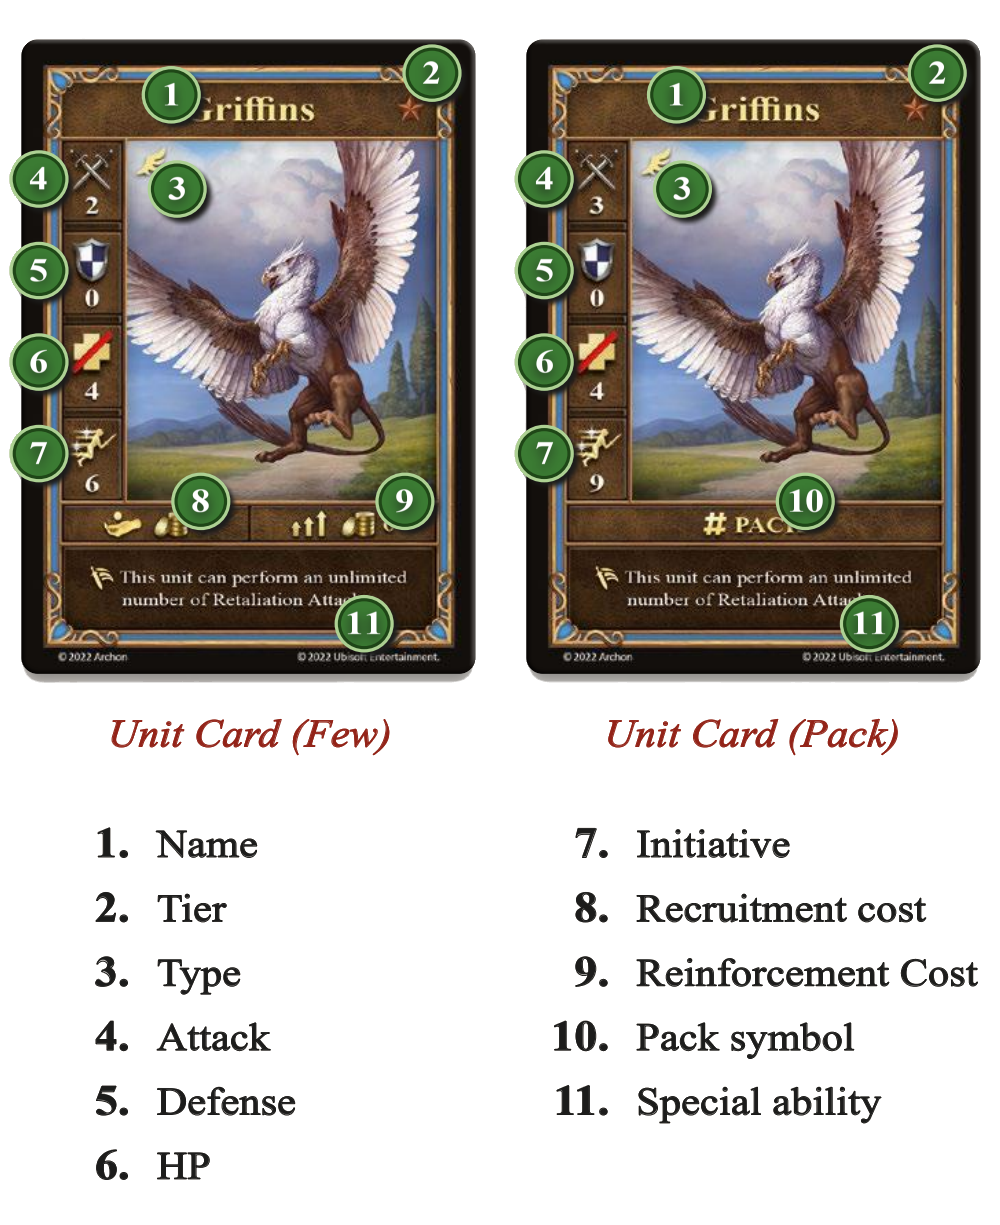
\includegraphics[width=\linewidth]{\cards/units.png}
\end{center}
\bigskip

\vspace*{\fill}

Most Units have a \textbf{special ability}\index{Special Ability}:\par
\begin{itemize}[wide]
  \item\textbf{Activation} \includesvg[height=10px]{\svgs/activation.svg} resolves when the Unit is Activated.
  \item\textbf{Attack} \includesvg[height=10px]{\svgs/unit_attack.svg} resolves when the Unit attacks during its Activation.
    In case of multiple attacks, resolve the effect for \textbf{the first attack only}.
  \item\textbf{Other} \includesvg[height=10px]{\svgs/unit_other.svg} may be resolved instead of the Unit's normal Activation.
    It replaces all movement and/or attacking.
  \item\textbf{Passive} \includesvg[height=10px]{\svgs/unit_passive.svg} resolves whenever its condition is met.
  \item\textbf{Retaliate} \includesvg[height=10px]{\svgs/unit_retaliate.svg} resolves when the Unit retaliates.
  \item In any other cases without one of the above icons, the unit's ability is used according to its text.
    Units may also use \hyperlink{Playerdecks}{these} symbols.
\end{itemize}

\vspace*{\fill}

\columnbreak

\subsection*{\hypertarget{Unittype}{Unit Types}}
There are three types of Units\index{Unit Types}:
\begin{itemize}
  \item \textbf{Ground} \includesvg[height=10px]{\svgs/unit_ground.svg} Units may move up to 3 spaces and then attack adjacent enemies.
  \item \textbf{Flying} \includesvg[height=10px]{\svgs/unit_flying.svg} Units may move up to 3 spaces, ignoring Combat Obstacles, and then attack adjacent enemies.
  \item \textbf{Ranged} \includesvg[height=10px]{\svgs/unit_ranged.svg} Units may attack any Unit anywhere and then move 1 space OR move up to 1 space without attacking.
\end{itemize}
If a \includesvg[height=10px]{\svgs/unit_ranged.svg} Unit is next to an enemy Unit, its attack target \textbf{must be} that adjacent enemy.
When attacking an adjacent enemy in this way, the \includesvg[height=10px]{\svgs/unit_ranged.svg} Unit suffers a Combat penalty\index{Combat Penalty}: throw two Combat Dice (instead of one) and \textbf{apply the smaller result}.\par
This penalty is also applied if the \includesvg[height=10px]{\svgs/unit_ranged.svg} unit attacks from its own backline into the enemy's backline.
Walls and Gates may also \hyperlink{Walls}{reduce} the damage from  \includesvg[height=10px]{\svgs/unit_ranged.svg} attacks.

\subsection*{Neutral Units}
Neutral Units\index{Neutral Units} guard the various locations on the Game Map.
Starting and winning Combat against them is necessary to Visit most Locations.
Neutral Units are spread into four different tiers, each with their own deck.
In addition to \includesvg[height=10px]{\svgs/bronze.svg}, \includesvg[height=10px]{\svgs/silver.svg} and \includesvg[height=10px]{\svgs/golden.svg}, there are also Azure \includesvg[height=10px]{\svgs/azure.svg} Neutral Units which are the strongest in the game.\par
Each of these decks should be kept separate from each other and shuffled during setup.
If a Neutral Unit Deck ever runs out of Cards, reshuffle the discard into a new deck.
When a Combat against Neutral Units starts, draw \hyperlink{Difficulty}{the appropriate number} of Units from each tier to take part in that Combat.\par
It is possible for players to gain Neutral Units to their unit deck through various effects, such as Scenario-Specific Rules or the Diplomacy Ability Card.
\textbf{Neutral Units cannot be Reinforced}, as they are single sided.
Whenever a Neutral Unit is defeated from anywhere, place it into the appropriate Neutral Discard Pile.\par
In \textbf{Clash} and \textbf{Alliance} Scenarios, Neutral Units are always controlled by the next enemy player sitting to your right.
When controlling Neutral Units in this way \textbf{they must always attack if possible}, or if they can't, move as close to an enemy unit as possible.\par

\end{multicols}

\begin{figure*}[!hb]
  \centering
  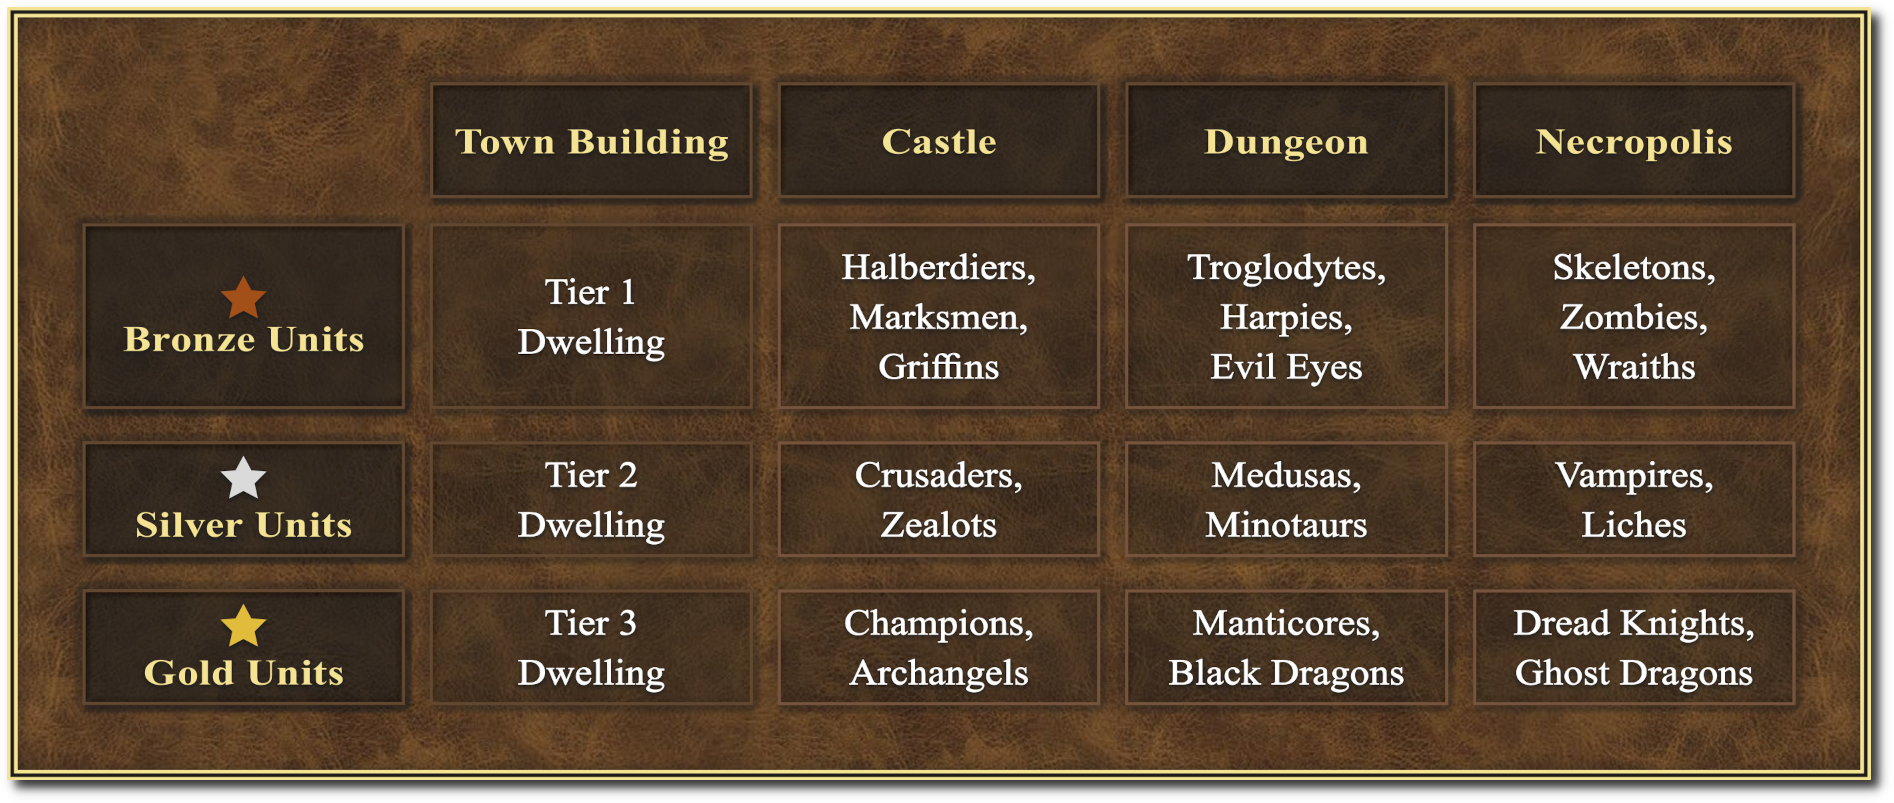
\includegraphics[width=\linewidth]{\tables/unit_list.png}
\end{figure*}

\clearpage

\subsection*{Example}

\begin{multicols}{2}

\textit{Alamar casts a Magic Arrow against Sandro's pack of Skeletons, Empowering \includesvg[height=10px]{\svgs/empower.svg} the Spell by two with the Expert  Effect \includesvg[height=10px]{\svgs/expert.svg} of a Power Card.}

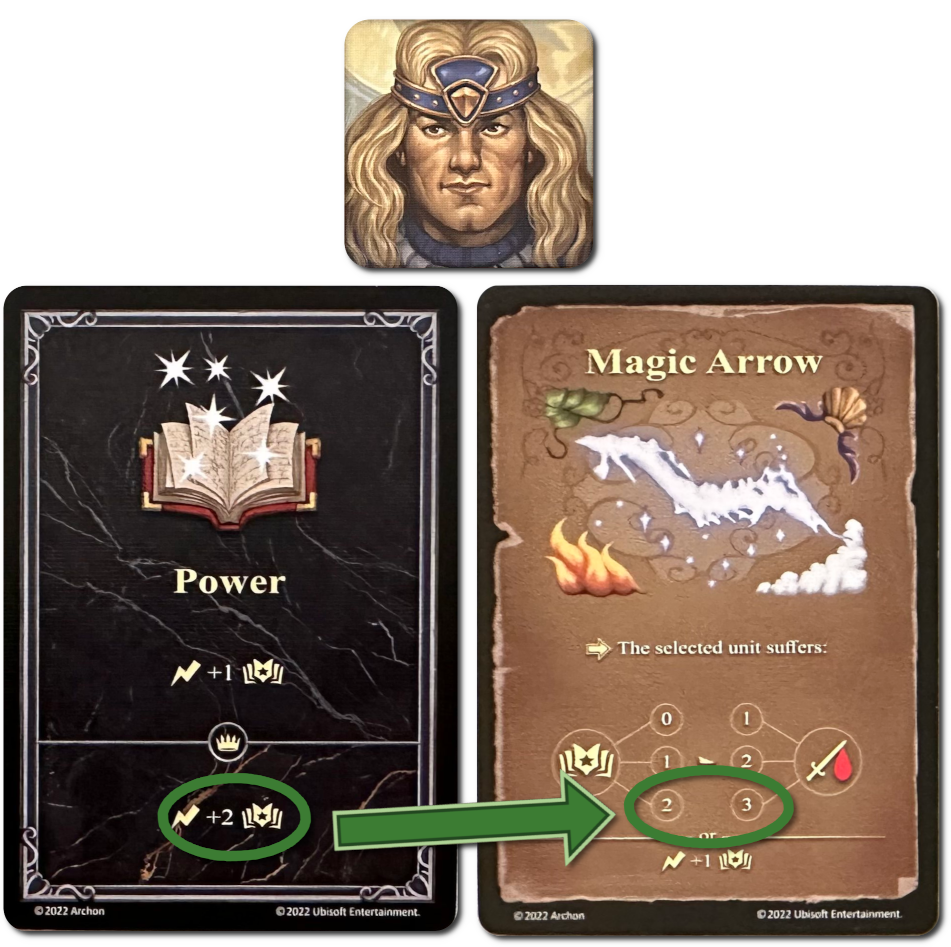
\includegraphics[width=\linewidth]{\examples/alamar_empowering_magic_arrow.png}
\par
\textit{
  The Skeletons take 3 damage \includesvg[height=10px]{\svgs/damage.svg} from the Spell.
  Their Defense \includesvg[height=10px]{\svgs/defense.svg} of 1 does not reduce the damage, because it only applies against attacks.
  The Skeletons have a HP \includesvg[height=10px]{\svgs/health_points.svg} of only 2, so they are now turned to their "Few" side and 1 leftover damage \includesvg[height=10px]{\svgs/damage.svg} is placed on them.
}
\par
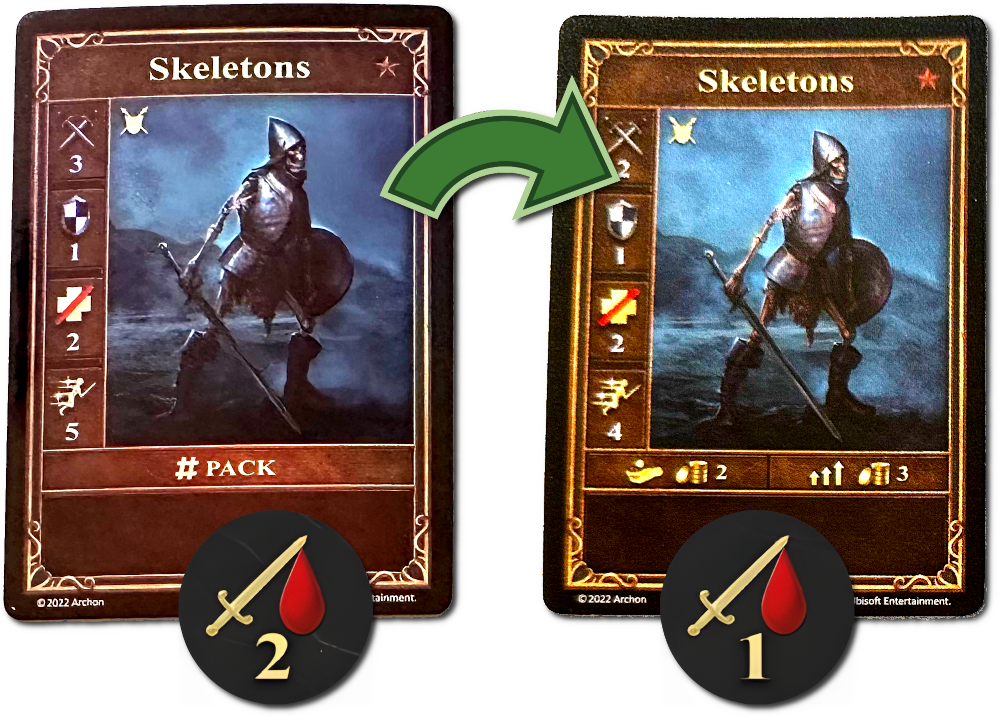
\includegraphics[width=\linewidth]{\examples/skeletons_flipped.png}

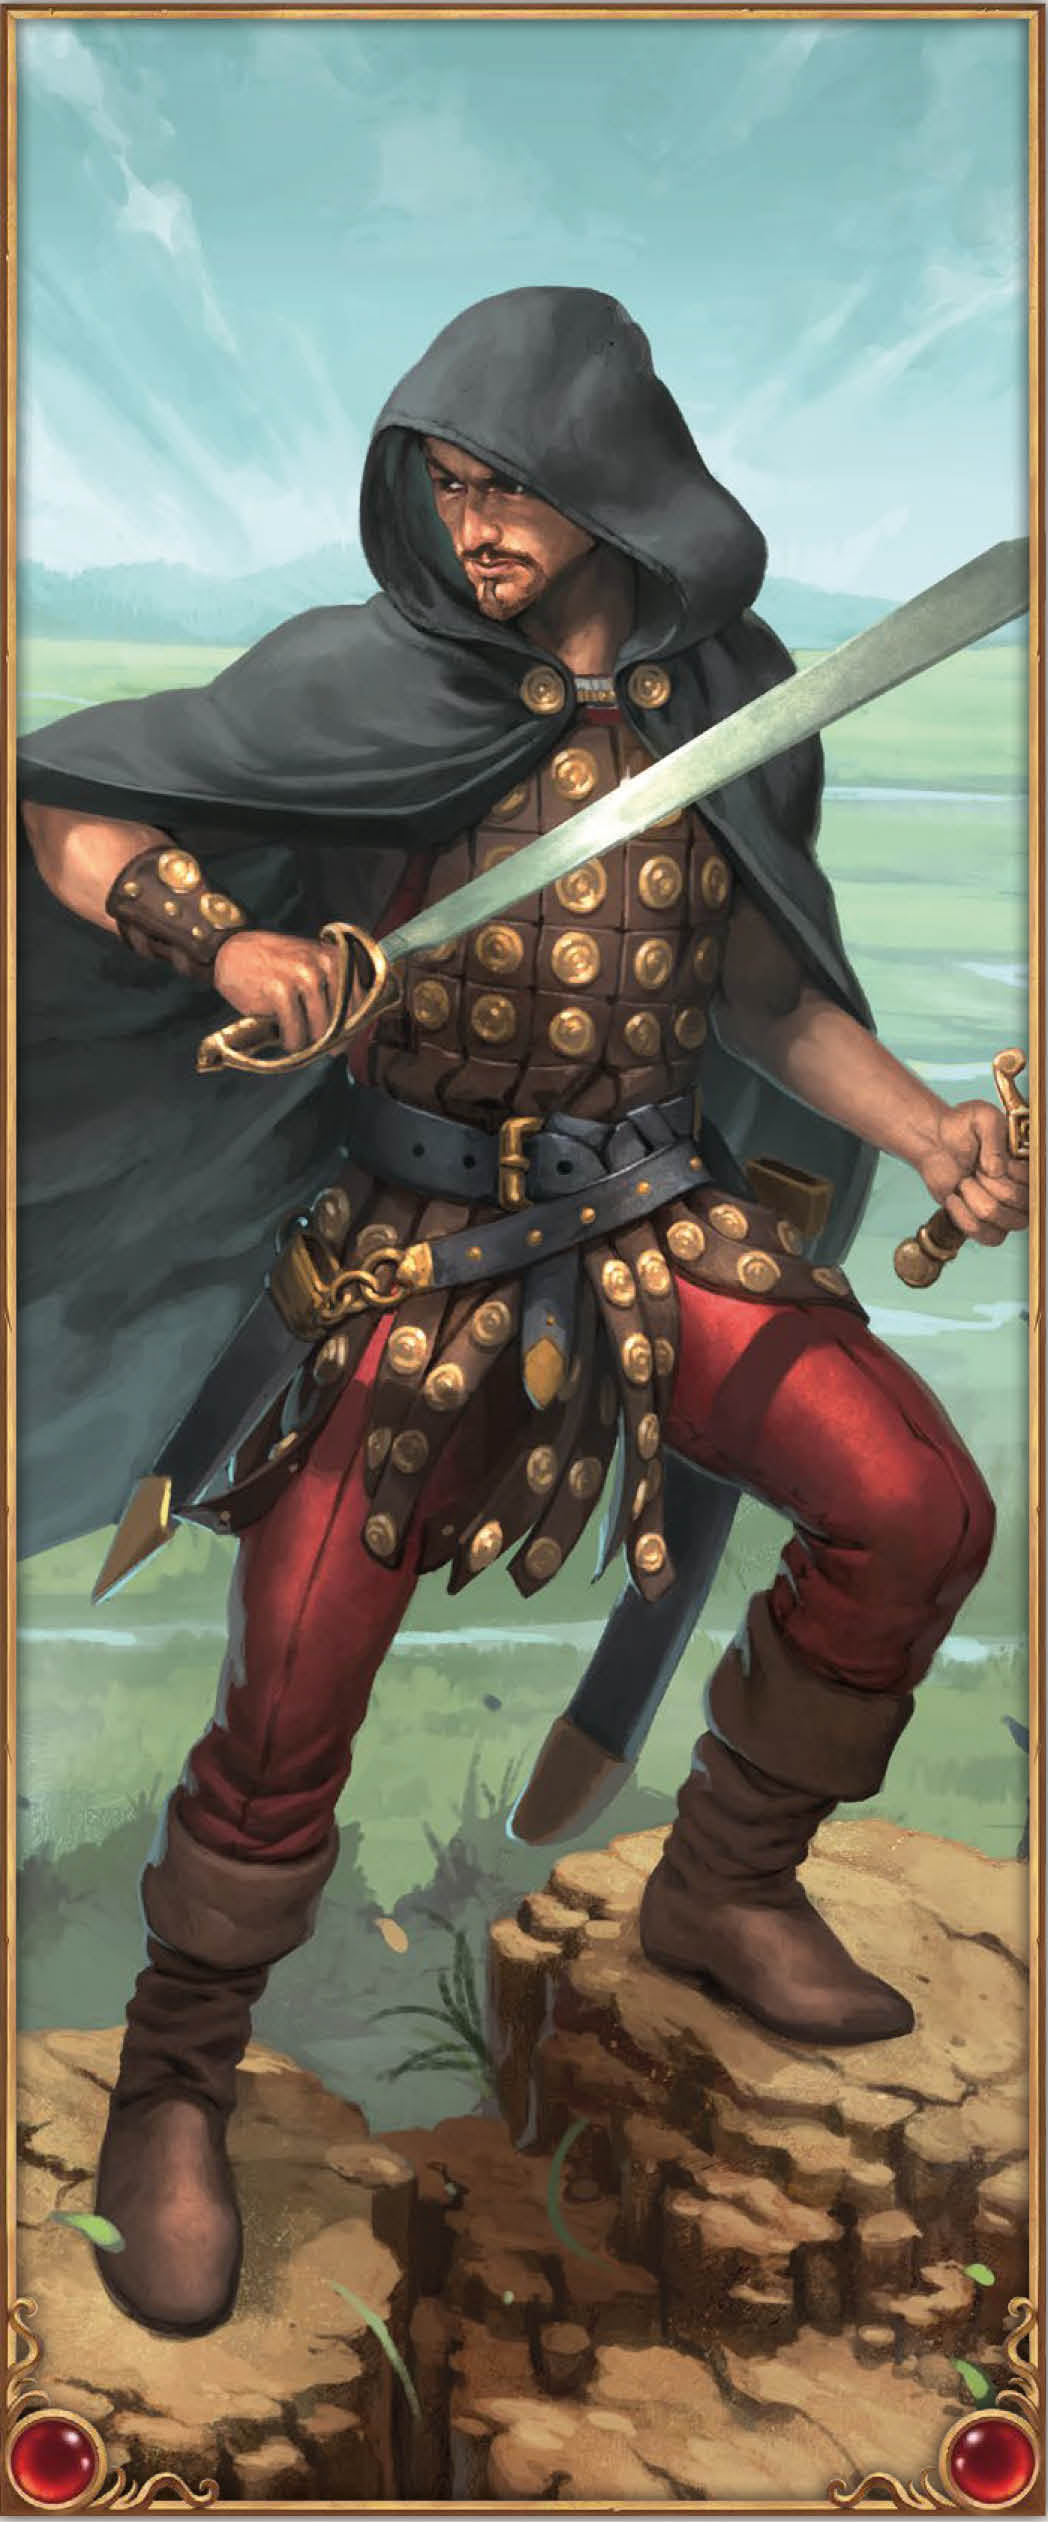
\includegraphics[width=\linewidth]{\art/rogue.jpg}

\end{multicols}


% !TeX spellcheck = en_US
\addsection{Combat}{\skills/attack.png}

\begin{multicols*}{2}

\hypertarget{Combat}{Combat} is resolved on the separate Combat Board.
Combat with \textbf{Neutral Units} starts when a Hero moves to an unvisited Field with a roman numeral, which signifies the \hyperlink{Difficulty}{type and number} of Neutral Units guarding that field.

Combat with \textbf{another player} can start in two ways:
\begin{itemize}
  \item You move into any Field containing one of their Heroes.
  \item You move into a Town or Settlement owned by them.
\end{itemize}
Players are able to start multiple combats during their turn.

\subsection*{\hypertarget{Combatsetup}{Combat setup}}

% TODO info about battlefield expansion
Combat takes place on the 4 x 5 Combat board, which consists of two Backlines and two Frontlines on opposite ends, and a middle row.
Follow these steps when Combat begins against \textbf{Neutral Units}:

\begin{itemize}
  \item Choose one of the Combat Board's sides as your own.
    Place up to 5 of your Unit cards freely onto the Back- and Frontline of that side.
  \item Check the \textbf{Difficulty Table} and draw the corresponding number of Neutral Unit cards from their decks.
  \item The Neutral Units are placed differently depending on the Game Mode:
  \item In \textbf{Clash} or \textbf{Alliance} Scenarios, the enemy player sitting to your right controls the Neutral Units and decides their placement.
    \includesvg[height=10px]{\svgs/unit_ranged.svg} Units must be placed in the backline if possible.
  \item In \textbf{Campaign} or \textbf{Co-op} scenarios, Neutral Units are placed from left to right from the player's perspective.
First, place any \includesvg[height=10px]{\svgs/unit_ranged.svg} units in the Backline.
Then, place any \includesvg[height=10px]{\svgs/unit_ground.svg} or \includesvg[height=10px]{\svgs/unit_flying.svg} Units in the Frontline.
If there's not enough room to place a Unit in its correct line, place them in the other one.
Units must be placed in decreasing Initiative order.
If there's a tie, place higher tier units first.
If there's still a tie, the players decide the placement order.
\end{itemize}
Unit setup when fighting \textbf{other players}:
\begin{itemize}[wide]
  \item The attacking player places up to 5 Units on their chosen side of the Combat Board, followed by the defender.
  \item If the combat takes place in a Town with a Citadel, the defender adds the \hyperlink{Walls}{Wall, Gate and Arrow Tower} cards after placing their Units.
\end{itemize}


\vspace*{\fill}
\hspace{6.6em}
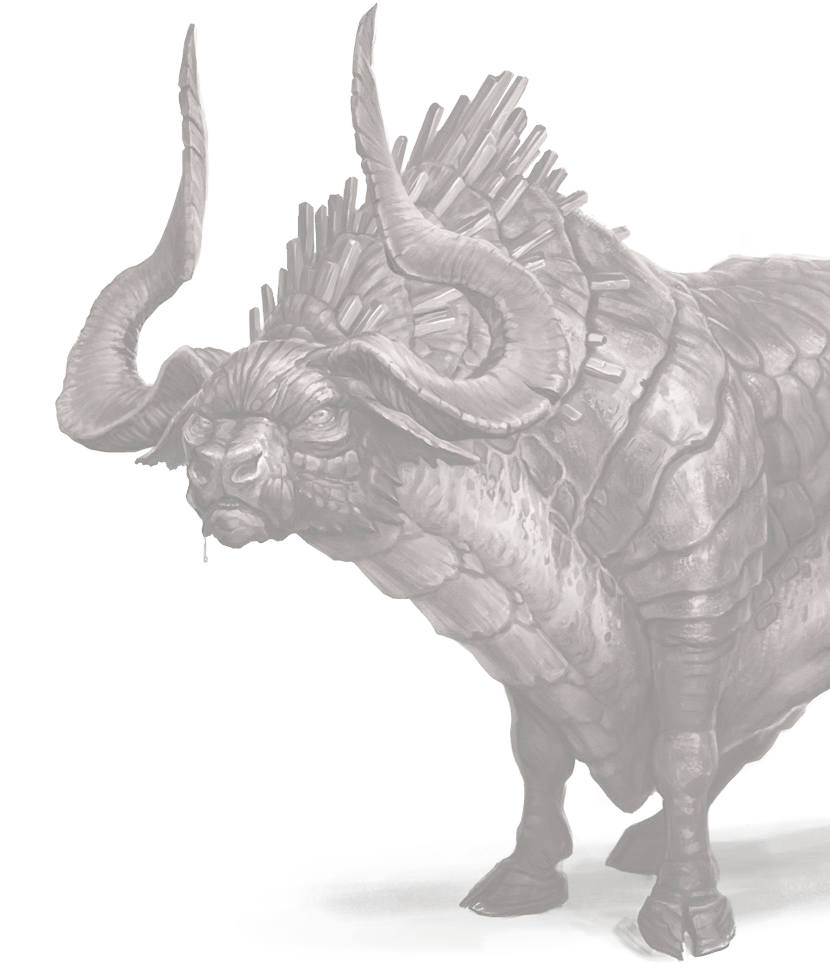
\includegraphics[width=0.9\linewidth]{\art/gorgone.png}

\vspace*{\fill}

\subsection*{\hypertarget{Combatterminology}{Combat Terminology}}
The following terms are used in this rule book and by the Unit and other cards to describe effects and elements during combat:\par
\textbf{Attacking playe}r – The player who started the Combat by moving their Hero.\par
\textbf{Defending player} – The player whom Combat was started against.\par
\textbf{Activation} – A Unit activates when it is next in the Initiative order.\par
\textbf{Adjacent Unit} – A Unit is directly adjacent to another if it is one space away in a cardinal direction (nondiagonal).\par
\textbf{Combat Round} – A full cycle of all Units of each player being Activated.\par
\textbf{Combat Obstacles} – Every card placed on the Combat Board counts as a Combat Obstacle.
Obstacles block the movement of all non-flying Units.\par
\textbf{Attack Die} – A red die whose results range from -1 to +1.
Roll the die whenever a unit attacks and
add the result to the unit's attack value.\par
\textbf{\hypertarget{Retaliate}{Retaliation Attack}} – If a unit survives an attack by an adjacent Unit, it performs an attack back on that Unit.
Each Unit can perform only 1 Retaliation Attack per Combat Round.
Retaliation Attacks function identically to normal attacks, but they cannot cause another Retaliation Attack.
Mark Units which have performed a Retaliation Attack this round with a black cube.\par
\textbf{Paralysis} \includesvg[height=10px]{\svgs/paralysis.svg} – Effects which paralyze a unit place the paralysis token on them.
A paralyzed Unit \textbf{skips its next Activation} and removes the token instead.
If it is \textbf{attacked or takes any damage} before that time, \textbf{remove the paralysis token} from that unit.\par
\textbf{\hypertarget{Defend}{Defend}} \includesvg[height=10px]{\svgs/defense.svg} – When a Unit with a Defense Token is attacked, make another roll with the attack die
after the initial attack roll.
If you roll a “+1”, the defending Unit gains an extra 1 defense for this attack.
If a Unit has a defense token at the start of its activation, discard it.
The Unit cannot take another defense action during that activation.

\subsection*{\hypertarget{CombatCards}{Using Cards During Combat}}
You may only use \textbf{one Spell per Combat Round}.
Other card types can be used as many times as you want to.
Ongoing \includesvg[height=10px]{\svgs/ongoing.svg} and \includesvg[height=10px]{\svgs/activation.svg} Activate effects can be used only when Activating one of your Units and before it attacks.
Ongoing effects last until end of Combat or if the effect on the card is used up.
Instant \includesvg[height=10px]{\svgs/instant.svg} Cards may be played at any time except between rolling the Combat Die and resolving damage unless otherwise stated.
Instant Cards which increase a unit's statistics \textbf{last only for the duration of the currently activated Unit's next attack}.
\subsection*{\hypertarget{Timelimit}{Combat Time Limits}}
Combat against Neutral Units has a time limit of \textbf{one Combat Round}.
If the player cannot win the Combat before the end of the current Combat Round, they must either \hyperlink{Endcombat}{Retreat} or spend 1 MP from the Hero that started the combat in order to play another Combat Round.\par
\textbf{Note}: Combat against Azure \includesvg[height=10px]{\svgs/azure.svg} Units, other players or \hyperlink{AIrules}{AI Heroes} have no time limit.

\vspace*{\fill}
\hspace{2em}
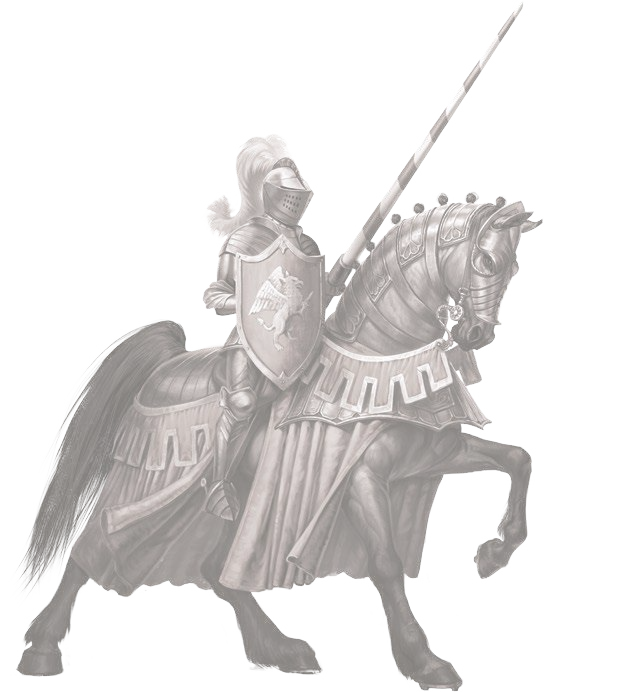
\includegraphics[width=0.9\linewidth]{\art/cavalryman.png}

\end{multicols*}

\begin{multicols}{2}

\subsection*{\hypertarget{Walls}{Defending a Town With a Citadel}}

When a Town with a Citadel is attacked, the defender adds the Wall and Gate Obstacles in any order to the Middle Row of the Combat Board after placing their Units.
The Gate Card is \textbf{not an Obstacle to the defending player}.
The Wall and Gate cards can be destroyed by any adjacent \includesvg[height=10px]{\svgs/unit_ground.svg} or \includesvg[height=10px]{\svgs/unit_flying.svg} Unit's attack.
Such attacks are always successful, do not roll the Combat Die when performing them.\par

Defending Units standing on their own side and \textbf{in the same column} as a Wall or a Gate are partially protected from \includesvg[height=10px]{\svgs/unit_ranged.svg} attacks.
If they are targeted by a \includesvg[height=10px]{\svgs/unit_ranged.svg} attack performed from the opponent's side of the Combat Board, \textbf{reduce the attack's damage by 1}.

\begin{center}
  \includegraphics[width=0.6\linewidth]{\cards/arrow_tower.png}
\end{center}
The defender also gains the Arrow Tower Unit Card which is placed next to the Combat Board.

\end{multicols}

\vspace*{\fill}

\begin{figure*}[!hb]
  \mbox{}%
  \hfill%
  \begin{minipage}[t]{0.4\textwidth}
    \centering
    \shadowimage[width=\linewidth]{\examples/ranged_protected.jpg}
  \caption[halberdiers protected]{\textit{Halberdiers are behind a non-destroyed Gate, they \textbf{are protected} when attacked from spaces 1-8.}}
  \end{minipage}
  \hfill%
  \begin{minipage}[t]{0.4\textwidth}
    \centering
    \shadowimage[width=\linewidth]{\examples/ranged_unprotected.jpg}
  \caption[halberdiers unprotected]{\textit{Because Halberdiers are not behind a non-destroyed Wall, \textbf{protection doesn't work}, regardless of where the \includesvg[height=10px]{\svgs/unit_ranged.svg} attack comes from.}}
  \end{minipage}
  \hfill%
  \mbox{}%
\end{figure*}

\begin{multicols}{2}

\subsection*{Combat Round Structure}
Combat is divided into Rounds, during which all of the Units participating in that Combat \textbf{Activate once} in Initiative order.
After each Unit has activated, a new Combat Round begins.
Combat lasts until all Units on one side are eliminated, a player has to \textbf{retreat} when fighting Neutral Units, or a player \textbf{Surrenders} to another player.

Structure of a combat round:
\begin{itemize}
  \item Players Activate their Units in decreasing order of Unit \hyperlink{Initiative}{Intiative}.
  \item When a unit Activates, place a Faction Cube on it to indicate it has been Activated this Combat Round.
  \item Activated Units may move and attack according to their \hyperlink{Unittype}{type}.
  \item Instead of attacking, a Unit may \hyperlink{Defend}{defend}.
  In Neutral Combat, the Neutral Enemy units cannot defend, even when controlled by another player.
  \item Before a Unit attacks, both players may \hyperlink{CombatCards}{play cards}. Cards are resolved in the order in which players decide to play them.
  \item After a Unit's attack has been declared and all cards have been played that the players wish to play, roll the Combat Die.
    Modify the attacking Unit's attack by the die's result, then reduce it by the defending Unit's defense, and finally deal the rest as \hyperlink{HP}{damage} to the defending Unit.
  \item If the defending Unit was adjacent to the attacker, it \hyperlink{Retaliate}{retaliates} if it hasn't done so this round.
  \item Keep activating Units until they've all been activated once.
After the last Unit's activation, the combat round ends.
\end{itemize}
\subsection*{\hypertarget{Endcombat}{End Of Combat}}
Combat can end in the following ways:
\begin{itemize}
    \item All Units on one side are defeated.
    \item A player runs out of time against Neutral Units and has to \textbf{Retreat}.
    \item A player \textbf{Surrenders} when fighting another player.
\end{itemize}
In combat against \textbf{Neutral Units}, if the player defeats all opposing Units they win the combat.
If the player \hyperlink{Timelimit}{runs out of time} or all of their Units are defeated, they instead have to \textbf{Retreat}; move any surviving Units back to your Unit Deck and move the Hero that started the Combat back to the Field they last Visited.
There are no other negative consequences.
\textbf{Important exception}: If \textbf{all} of your Units from your Unit Deck were defeated during that Neutral Combat, your Main Hero must instead be moved to a friendly Town or Settlement. Secondary Heroes are removed from the game until Recruited again.\par
If you defeat all Units \textbf{during combat against another player's Main Hero}, the defeated player \textbf{loses Morale} and has to \textbf{pay the winner} 5 \includesvg[height=10px]{\svgs/gold.svg}.
Do not lose Morale or pay \includesvg[height=10px]{\svgs/gold.svg} if a \textbf{Secondary Hero} is defeated.
\textbf{In both cases}, the defeated player also \textbf{gives the winner} one of their \hyperlink{End}{faction cubes}.
Defeated Main Heroes \textbf{have to move} to a friendly Town or Settlement, while Secondary Heroes are removed from the game until Recruited again.\par
You may \textbf{Surrender} to other players by paying the other player 10 \includesvg[height=10px]{\svgs/gold.svg} when activating a Unit.
Move your Main Hero or remove your Secondary Hero from the game as if you were defeated by losing your Units.
There are no other direct consequences to Surrendering; the winner does not gain a Faction Cube.
\textbf{Note}: You cannot surrender when defending a Town.\par
When a Secondary Hero is attacked, they may also choose to be \textbf{instantly defeated} instead of fighting a Combat in order to preserve their Units.
When this happens, the attacker still receives a Faction Cube from the defeated Hero.
Defeating a Main Hero \hyperlink{End}{may eliminate} that player.\par
When Combat ends, all damage is healed from all surviving Units.
Move any player owned Units back to their Unit Deck and discard any leftover enemy Neutral Units.
After winning Combat, Heroes \textbf{must} Visit the Field where the Combat took place.

\subsection*{\hypertarget{Combatexperience}{Combat Experience}}

Winning Combat with your Main Hero usually grants them Experience.
If either the Difficulty of the Neutral Field or the Level of a defeated enemy Main Hero was equal to your Level, gain 1 \includesvg[height=10px]{\svgs/exp.svg}.
If they were higher than your Level, gain 2 \includesvg[height=10px]{\svgs/exp.svg}.
Winning a Neutral Combat which involved an Azure \includesvg[height=10px]{\svgs/azure.svg} Unit grants your Hero Level 7 immediately.
If you gain multiple Levels in this way, resolve their effects in order.\par
Secondary Heroes cannot ever gain Experience.
You also \textbf{do not gain} Experience from defeating a Secondary Hero, or if an enemy Hero Surrenders to you.
\subsection*{\hypertarget{Quick}{Quick Combat}}
If your Hero's Level is higher than a Field's Difficulty when Combat against Neutral Units would begin, \textbf{no Combat} takes place.
The player is considered to have beaten the Neutral Units by default and gains no rewards from the Combat.

\subsection*{\hypertarget{AIrules}{Player vs AI}}
These rules apply when playing a \textbf{Solo} game.
The AI Combat rules for targeting and attacking are also used when playing a \textbf{Cooperative} Scenario.\par
Solo Campaigns are played against AI Heroes who use two automated decks to play the game: the AI Deck, and the Spell Deck.
The AI Deck consists of cards that are similar in function to Abilities and Artifacts, but change depending on the game's \hyperlink{Difficulty}{Difficulty}.
The Spell Deck should be used when instructed by the cards in the AI Deck.
During combat against Neutral enemies or AI Heroes, their Units follow an automatic set of instructions.
\textbf{Initiative rules} work identically.
When an \textbf{AI hero} Activates a Unit, draw an AI card and follow its instructions as the Unit's Activation.\par
All AI controlled \includesvg[height=10px]{\svgs/unit_ground.svg} and \includesvg[height=10px]{\svgs/unit_flying.svg} Units prioritize attacking Units of the same tier.
If this is impossible, they attack the closest Unit, prioritizing the lowest tier one.
\includesvg[height=10px]{\svgs/unit_ranged.svg} Units prioritize attacking other \includesvg[height=10px]{\svgs/unit_ranged.svg} Units of the same tier, then lower tier, and finally higher tier.
If there are no \includesvg[height=10px]{\svgs/unit_ranged.svg} Units for them to target they prioritize \includesvg[height=10px]{\svgs/unit_ground.svg} and \includesvg[height=10px]{\svgs/unit_flying.svg} Units in the same tier order.
If there's more than one valid target, they attack the closest one.\par
If there's ever a tie between equally valid targets for any units, the players choose which Unit is attacked.

\textbf{AI Ueroes} always start in their Town's Field unless otherwise stated.
They have 3MP and always use them to perform the following actions in decreasing priority:
\begin{itemize}
  \item Check if a player Hero is on the same Tile as the AI.
    If they are, spend all MP to move towards them in an attempt to begin Combat.
  \item Check if there are any Mines or Settlements to Flag on the Map Tile the AI Hero is on.
    If there are any, move toward the closest one and Flag it.
  \item Otherwise, move toward the player's Town in an attempt to Flag it.
Repeat this sequence until all MP is used.
\end{itemize}

\begin{center}
  \includegraphics[width=\linewidth]{\cards/ai.png}
\end{center}

AI Heroes always \textbf{automatically win Combat} against any Neutral Units, while simultaneously \textbf{Flagging or Visiting all fields} they happen to move through.
They gain no benefits from Flagging or Visiting Fields.

AI Heroes must discover face down Map Tiles as normal by spending 1 MP before moving onto them.
The player chooses that tile's orientation.\par
AI Heroes cannot Surrender and you cannot Surrender to them;
they will always fight until they run out of Units.
Winning Combat against an AI Hero does not grant any rewards unless stated by the Scenario.
AI Heroes do not have a Town Board, Resources, or a Hero Card.
Their Units are static and defined by the Scenario's set up or other rules.\par
Any differences to the above will be described in any given Scenario's own rules.


\end{multicols}

\vspace*{\fill}
\begin{scaledfigure}[blanker]
  \centering
  \includegraphics[width=\linewidth, height=\myspace, keepaspectratio]{\art/sharpshooter.jpg}
\end{scaledfigure}

\clearpage

\begin{multicols}{2}
\textit{Sandro's Zombies are about to attack Catherine's Griffins.
As Sandro announces the attack, both players now have a chance to modify the attack or defense of their own Unit by playing any number of \includesvg[height=10px]{\svgs/instant.svg} cards that increase an attacking Unit's \includesvg[height=10px]{\svgs/attack.svg} or a defending Unit's \includesvg[height=10px]{\svgs/defense.svg}.}\par
\textit{Sandro decides to play a +1 Attack Card, increasing the Zombies' attack from 2 to 3.
Catherine responds by playing a +1 Defense Card, increasing the Griffins' defense from 0 to 1.
They would both be permitted to play any amount of additional cards in any order, but they decide to stop after playing these cards.}\par
\textit{After all cards for the attack have been played, the Attack Die is thrown to further modify the amount of damage the attacking Unit deals.
Sandro throws a +1.
This increases the Zombies' attack from 3 to 4, which is then reduced by the Griffins' defense of 1. Therefore, 3 damage \includesvg[height=10px]{\svgs/damage.svg} is placed on the Griffins. Since they have a HP \includesvg[height=10px]{\svgs/health_points.svg} of 4, they are not removed from the Combat.}\par
\textit{The Griffins do not have a black cube on them, therefore they now start a Retaliation Attack.
The cube would now normally be placed on them, however their Special \includesvg[height=10px]{\svgs/unit_retaliate.svg} Ability indicates that they may Retaliate any number of times so the cube is not placed.}\par
\textit{Relatiation Attacks work identically to a normal attack, with the exception that they do not cause another Retaliation Attack.
Therefore, both players are now allowed to modify the statistics of their units again.
The previously played Attack and Defense cards no longer have any effect.}

\end{multicols}

  \begin{minipage}{0.8\textwidth}
    \centering
    \includegraphics[width=\linewidth]{\examples/zombies_attack_griffins.png}
\end{minipage}


% !TeX spellcheck = en_US
\addsection{Scenario End}{\skills/archery.png}

\begin{multicols*}{2}

\hypertarget{End}{All} Scenarios have their victory conditions\index{Victory Conditions} described in the Scenario Book.
In addition, it is always possible to be \textbf{Eliminated} from any Scenario in the following ways:
\begin{itemize}
  \item Play 3 full Rounds without controlling a Town or a Settlement.
    Count the number of Rounds left using any suitable component.
  \item Lose Combat with your \textbf{Main Hero} when you have no Towns or Settlements left, including when defending your last Town or Settlement.
\end{itemize}
Eliminated players are immediately removed from the game.
Discard their Faction Cubes and Hero models from the Game Map.
Treat the cards in their Deck as being Removed from the game for the rest of the Scenario.
If you are Eliminated, you may still participate in the game by controlling Neutral Units.\par
\note{4}{If you Eliminate all enemy Factions, you immediately win the Scenario.}\par

In \textbf{Clash} Scenarios with three or more players, collecting \textbf{a Faction Cube} from every enemy player immediately wins you the game.
Other Scenario specific rules may also modify the outcome of collecting Faction Cubes.

\columnbreak

After finishing a \textbf{Solo Campaign} scenario, reset your Hero's Experience Level to 1, and prepare the starting deck for the next scenario of the campaign.
It will consist of:
\begin{itemize}
  \item all the \hyperlink{Statistic}{Statistic} cards from your deck,
  \item the level 1 \hyperlink{Specialty}{Specialty} card,
  \item 5 other non-Specialty cards of your choice from your deck.
\end{itemize}
Skip steps 11-13 of Setup for the next scenario of the campaign.

\vspace*{\fill}
\hspace{-3em}
\includegraphics[width=1.7\linewidth]{\art/medusa.png}

\end{multicols*}


% !TeX spellcheck = en_US
\addsection{Other Rules}{\skills/armorer.png}
\begin{multicols}{2}

\subsection*{\hypertarget{Trading}{Trading}}

The \hyperlink{Trading Post}{Trading Post Field} and other effects allow you to trade Resources with the game in accordance to the table below.
You may also \textbf{Remove cards} from your hand at the trading post to gain 1 \includesvg[height=10px]{\svgs/gold.svg} per card.
\textbf{Note}: Specialty, Statistic, Starting Ability and Magic Arrows \textbf{cannot be removed} in this way.\par
In \textbf{Alliance} and \textbf{Cooperative} Scenarios, players are allowed to trade Resources and cards following these rules:
\begin{itemize}
  \item In Alliance Scenarios, allies may trade Resources freely at any time on their turns except during Combat.
  \item In Cooperative Scenarios, Resources may be given to other players when visiting a Trading Post.
  \item In both Scenario types, allies may trade \textbf{Spell} and \textbf{Artifact} cards in any mix if they have heroes on adjacent Fields.
    Only \textbf{cards from their hands} may be traded and you must give and receive an equal amount of cards.
\end{itemize}

\vspace*{\fill}
\includegraphics[width=\linewidth]{\art/ammo_cart.png}

\end{multicols}

\vfill
\begin{figure*}[!hb]
  \centering
  \includegraphics[width=\linewidth]{\tables/trade_table.png}
\end{figure*}
\vfill

\clearpage

\begin{multicols}{2}

\subsection*{\hypertarget{Difficulty}{Difficulty}}
During setup, players must choose the game's Difficulty.
There are four different Difficulties, each with a different starting bonus that players receive during setup:
\begin{itemize}
  \item \textbf{Easy} – Roll 2 \includesvg[height=10px]{\svgs/resource_die.svg} and receive Resources from both – OR – \textbf{Search} (2) the Artifact deck, twice.
  \item \textbf{Normal} – Roll 2 \includesvg[height=10px]{\svgs/resource_die.svg} and receive the Resources from one of them – OR – \textbf{Search} (2) the artifact deck.
  \item \textbf{Hard} – Roll 1 \includesvg[height=10px]{\svgs/resource_die.svg} and receive the Resources on it – OR – reveal cards from the top of the Artifact Deck until you find 1 Minor Artifact and add it to your hand.
  \item \textbf{Impossible} – No starting bonus.
\end{itemize}
All \textbf{Artifacts} received from a starting bonus should be placed into your \textbf{hand} and not shuffled into your Starting Deck.
Shuffle the Artifact Deck and its Discard Pile together afterwards, and then discard one Artifact from the top to form the Artifact Discard Pile again.\par
The chosen difficulty also determines the number and type of neutral enemies that are encountered during Neutral Combat:

\end{multicols}

\vfill
\begin{figure*}[!hb]
  \centering
  \includegraphics[width=\linewidth]{\tables/field_difficulty.png}
\end{figure*}
\vfill


% !TeX spellcheck = en_US
\addsection{Expansion Content}{\skills/pathfinding.png}

\begin{multicols}{2}

\subsection*{Schools of Magic}
Most expansions have effects which refer to Schools of Magic.
All Spell Cards belong to one School: either Air, Fire, Earth or Water.
When casting the \textbf{Magic Arrow Spell}, you must select which School it belongs to.
\textbf{Hero specialty cards are not spells} even though some of them have a School of Magic.
Spells with four School symbols on them are \textbf{Expert Spells}, which may be referred to by certain effects.

\columnbreak

\begin{minipage}[t]{0.48\textwidth}
  \centering
  \minipage[b]{0.5\textwidth}
    \centering
    \includegraphics[width=0.75\linewidth]{\images/school_of_fire.png}
    \textit{\textbf{\textcolor{darkcandyapplered}{School of Fire}}}
  \endminipage
  \minipage[b]{0.5\textwidth}
    \centering
    \includegraphics[width=0.75\linewidth]{\images/school_of_water.png}
    \textit{\textbf{\textcolor{darkcandyapplered}{School of Water}}}
  \endminipage
  \hfill\allowbreak%
  \bigbreak
  \minipage[b]{0.5\textwidth}
    \centering
    \includegraphics[width=0.75\linewidth]{\images/school_of_air.png}
    \textit{\textbf{\textcolor{darkcandyapplered}{School of Air}}}
  \endminipage
  \minipage[b]{0.5\textwidth}
    \centering
    \includegraphics[width=0.75\linewidth]{\images/school_of_earth.png}
    \textit{\textbf{\textcolor{darkcandyapplered}{School of Earth}}}
  \endminipage
  \bigbreak
\end{minipage}

\end{multicols}

\begin{multicols*}{2}

\begin{center}
  \includegraphics[width=0.5\linewidth]{\art/land_mine.png}
\end{center}

\subsection*{War machines}
Added by the Rampart expansion.
War Machines are permanent cards that can be bought at either a Trading Post or a War Machine Factory.
If you buy one at the Trading Post, \textbf{you cannot use} any of the other normal functions of that Field during that visit.
War machines are also more expensive at the Trading Post.\par
\medskip
\begin{minipage}[h]{\linewidth}
  \begin{center}
    \textbf{War Machine Factory}\medskip
  \end{center}
  \shadowimage[width=\linewidth]{\map_locations/war_machine_factory.jpg}
  \footnotesize{Category: \textbf{Revisitable}\\This location allows a Hero to buy a War Machine.}
\end{minipage}

\bigskip

\begin{minipage}[h]{\linewidth}
  \vspace{0pt}
  \centering
  \begin{scriptsize}
    \begin{tikzpicture}
      \draw (0, 0) node[inner sep=0] {\makebox[\textwidth][c]{\includegraphics[width=0.8\textwidth]{\cards/war_machine.png}}};
      \draw (0.8, 3.6) node {\encircle{\phantom{.}1\phantom{.}}};
      \draw (0, -2.8) node {\encircle{\phantom{.}2\phantom{.}}};
      \draw (-1.2, -1.7) node {\encircle{\phantom{.}3\phantom{.}}};
      \draw (0.9, -1.7) node {\encircle{\phantom{.}4\phantom{.}}};
    \end{tikzpicture}
  \end{scriptsize}
  \break
  \footnotesize{\textbf{\textit{\textcolor{darkcandyapplered}{War Machine Card}}}}
  \scriptsize
  \begin{multicols}{2}
    \begin{itemize}
      \item[\textbf{1.}] \textbf{Name}
      \item[\textbf{2.}] \textbf{Effect}
      \item[\textbf{\phantom{.}}] \phantom{.}
      \item[\textbf{3.}] \textbf{War Machine Factory cost}
      \item[\textbf{4.}] \textbf{Trading Post cost}
    \end{itemize}
  \end{multicols}
\end{minipage}

\subsection*{Permanent cards}
Added by the stretch goals and Rampart expansions, explained \hyperlink{Playerdecks}{here}.

\subsection*{Events}
Added by the Fortress expansion.
Event cards may be used in games with more than one player.
Shuffle the Event Deck during setup.
At the start of each Resource Round (except the first Round), draw and read the next Event Card after receiving Resources.
The first Event is drawn by the starting player.
\textbf{Change this player in a clockwise order} every time a new Event is drawn.
Resolve any effects in clockwise order starting with the player who drew the Card.
Any cards which were revealed as a part of resolving an Event should be shuffled back into their respective Decks afterwards.

\medskip

\begin{minipage}[h]{\linewidth}
  \vspace{0pt}
  \centering
  \begin{scriptsize}
    \begin{tikzpicture}
      \draw (0, 0) node[inner sep=0] {\makebox[\linewidth][c]{\includegraphics[width=\linewidth]{\cards/event.png}}};
      \draw (1, 1.8) node {\encircle{\phantom{.}1\phantom{.}}};
      \draw (-2, 0.4) node {\encircle{\phantom{.}2\phantom{.}}};
      \draw (2.5, -1.1) node {\encircle{\phantom{.}3\phantom{.}}};
    \end{tikzpicture}
  \end{scriptsize}
  \footnotesize{\textbf{\textit{\textcolor{darkcandyapplered}{Event Card}}}}
  \scriptsize
  \begin{multicols}{2}
    \begin{itemize}
      \item[\textbf{1.}] \textbf{Name}
      \item[\textbf{2.}] \textbf{Fluff}
      \item[\textbf{3.}] \textbf{Effect}
      \item[\textbf{\phantom{.}}] \phantom{.}
    \end{itemize}
  \end{multicols}
\end{minipage}

\subsection*{Summoning}
Some cards from the Inferno expansion may Summon Units during Combat.
Place the summoned Unit adjacent to the summoning Unit.
Summoned Units Activate in the round they were summoned if their initiative is lower or equal to the Initiative of the currently Activated Unit.
Otherwise, treat them as if they already activated this Combat Round.
After Combat, unless stated otherwise, the Summoned Units are added to your Unit Deck.

\subsection*{Empowered Statistic Cards}
Added by the Inferno expansion.
These cards are more powerful versions of the normal Statistics cards.
They have only one effect which is identical to the normal Statistic's Expert Effect, but does not require using your \includesvg[height=10px]{\svgs/expert.svg}.

\begin{center}
  \includegraphics[width=\linewidth]{\cards/empowered_statistics.png}
\end{center}

\subsection*{Random town}
Added by the Inferno expansion.
When this field is revealed, all players roll 2 \includesvg[height=10px]{\svgs/resource_die.svg}.
The highest roller chooses an unused faction.
The random town is defended by units from that faction.
They have a pack of bronze, two packs of silver, and two "fews" of gold units.
Flagging it increases gold production by 10, which is also gained immediately if you are the first to flag it.

\bigskip

\begin{minipage}[h]{\linewidth}
  \begin{center}
    \textbf{Random Town}\medskip
  \end{center}
  \shadowimage[width=\linewidth]{\map_locations/random_town.jpg}
  \small{Category: \textbf{Flaggable}}
\end{minipage}

\end{multicols*}


% !TeX spellcheck = en_US
\addsection{All Map Locations}{\skills/earth_magic.png}

\begin{multicols*}{2}

\hypertarget{All}{This} section describes the function of every single Field in the game.
The vast majority of Fields have useful iconography that clearly communicates the Field's effect.
On the right is a screenshot of the back of the rule book that explains these.
If a Field has any combination of these icons and is not described in detail later, then that Field is either \textbf{Visitable} or \textbf{Flaggable} and its only effect is indicated by these icons.\par
Revisitable Fields do not have an icon that indicates them to be such.
For this reason all Revisitable Fields are pictured and described individually.
The \includegraphics[height=0.8\baselineskip]{\images/revisitable.png} symbol is on almost all Flaggable Fields, with the major exception of Settlements.
Rules for Flagging Mines, Settlements and Towns are on the next page followed by descriptions of Revisitable and unique Fields marked with a question mark.\par
Random Towns and War Machine Factories are explained above.

\vfill
\begin{center}
  \hspace{-14em}
  \includegraphics[width=0.8\linewidth]{\art/ballista.png}
\end{center}

\begin{center}
  \framedimage[\linewidth]{\tables/symbols.png}
\end{center}

\clearpage
\subsection*{Towns, Mines and Settlements}
\textbf{Towns} are always located in the center of a starting tile.
Flagging an enemy Town prevents their Secondary Heroes from spawning there and Main Heroes from moving there if defeated.
Flagging a Town can cause \hyperlink{End}{player elimination}, and Scenarios typically have special rewards for Flagging them.
Flagging a Town also gives you a Faction Cube from its original owner.
Otherwise, Flagging a Town does not affect its original owner in any way.
They do not lose access to their Town board or its functions.
You also do not gain access to their Town board or Faction Units, unlike in the video game.
You can \hyperlink{Town}{pay Gold} to defend Towns with your Units if you Hero is not there when it is attacked.

\begin{center}
  \framedimage[\linewidth]{\images/core_towns.jpg}
  \textit{Towns from the core game.}
\end{center}

\medskip

\hypertarget{Mines}{\textbf{Mines}}\index{Mines} are Flaggable Fields which increase a specific resource's income when Flagged.
If you are the first one to Flag a mine, it also immediately provides you with its income.

\begin{center}
  \includegraphics[width=0.6\linewidth]{\images/mine_example.png}\\
  \textit{A mine that produces \includesvg[height=10px]{\svgs/valuablegreater.svg}, guarded by Level 3 neutrals.
    The first player to Flag this Field would immediately gain one \includesvg[height=10px]{\svgs/valuablegreater.svg} in addition to increasing their \includesvg[height=10px]{\svgs/valuablegreater.svg} income.
    All Mines are recognizable by the \includegraphics[height=0.8\baselineskip]{\images/revisitable.png} symbol.
  }
\end{center}

\textbf{Settlements}\index{Settlement} function similarly to both Towns and Mines.
They act as a spawn point for Secondary Heroes, and as a place for Main Heroes to move to when defeated.
You may also \hyperlink{Town}{pay Gold} to defend Settlements with Units.
When you Flag a Settlement, you choose whether to increase your \includesvg[height=10px]{\svgs/gold.svg}, \includesvg[height=10px]{\svgs/building_materials.svg} or \includesvg[height=10px]{\svgs/valuablegreater.svg} income by one space.
As with Mines, if you are the first player to Flag a Settlement, you immediately gain resources equal to that increase in production.
Mark the Settlement with an appropriate Resource Token to show which resource it produces.
When you Flag an enemy Settlement you may switch which resource it produces.\par
Additionally, \textbf{instead of increasing Resource Production}, you may choose to \textbf{Reinforce} one of your \includesvg[height=10px]{\svgs/bronze.svg} or \includesvg[height=10px]{\svgs/silver.svg} Units immediately for half the normal cost, rounded up.
If you were the first player to flag the Settlement, Reinforce that Unit \textbf{for free} instead.
Do not place any Resource Tokens on the Settlement if you choose to Reinforce.

\bigbreak

\begin{minipage}[h]{\linewidth}
  \centering
  \includegraphics[width=0.44\linewidth]{\map_locations/castle_settlement.png}
  \includegraphics[width=0.44\linewidth]{\map_locations/dungeon_settlement.png}
  \includegraphics[width=0.44\linewidth]{\map_locations/necropolis_settlement.png}
  \includegraphics[width=0.44\linewidth]{\map_locations/rampart_settlement.png}
  \includegraphics[width=0.44\linewidth]{\map_locations/fortress_settlement.png}
  \includegraphics[width=0.44\linewidth]{\map_locations/inferno_settlement.png}
  \includegraphics[width=0.4\linewidth]{\map_locations/tower_settlement.png}
  \par
  \textit{All possible Settlements.
  Each is styled after a different Faction.
  They all work identically.}
\end{minipage}
\end{multicols*}
\bigbreak

\subsection*{Revisitable Fields}

\begin{figure}[H]
  \begin{minipage}[t]{0.47\textwidth}
    \vspace{0pt}
    \centering
    \textbf{Library}\par
    \framedimage[\textwidth]{\map_locations/library.jpg}
    \caption{\small Category: \textbf{Revisitable}\\You may
      \includesvg[height=8px]{\svgs/pay_v2.svg}
      3 \includesvg[height=8px]{\svgs/gold.svg}
      to Remove 1 Statistic Card from your hand or Discard Pile and replace it with any other Statistic Card.
      You may do this twice per Visit.}
  \end{minipage}\hfill
  \begin{minipage}[t]{0.47\textwidth}
    \vspace{0pt}
    \centering
    \captionsetup{singlelinecheck=off}
    \phantom{j}\textbf{Black Market}\par
    \framedimage[\textwidth]{\map_locations/black_market.jpg}
    \caption[black market]{\small Category: \textbf{Revisitable}\\Look at the top 4 cards from the Artifact Discard Pile.
      You may buy one of them for:
      \begin{itemize}
      \setlength\itemsep{-4pt}
        \item [5] \includesvg[height=8px]{\svgs/gold.svg} if it is a \textbf{Minor} Artifact
        \item [7] \includesvg[height=8px]{\svgs/gold.svg} if it is a \textbf{Major} Artifact
        \item [10] \includesvg[height=8px]{\svgs/gold.svg} if it is a \textbf{Relic} Artifact
      \end{itemize}
      }
  \end{minipage}
\end{figure}

\begin{figure}[H]
  \begin{minipage}[t]{0.47\textwidth}
    \vspace{0pt}
    \centering
    \textbf{Sanctuary}\par
    \framedimage[\textwidth]{\map_locations/sanctuary.jpg}
    \caption{\small Category: \textbf{Revisitable}\\
      Heroes on this Field cannot be attacked by other Heroes.
      Friendly Heroes can move through enemy Heroes on this Field but cannot stop here.}
  \end{minipage}\hfill
  \begin{minipage}[t]{0.47\textwidth}
    \vspace{0pt}
    \centering
    \phantom{j}\textbf{Tavern}\par
    \framedimage[\textwidth]{\map_locations/tavern.jpg}
    \caption{\small Category: \textbf{Revisitable}\\
      You can \includesvg[height=8px]{\svgs/pay_v2.svg}
      7 \includesvg[height=8px]{\svgs/gold.svg}
      to gain a Secondary Hero.
      Place their model on this Field.
      Then, choose one enemy player to discard 1 random card from their hand.}
  \end{minipage}
\end{figure}

\begin{figure}[H]
  \begin{minipage}[t]{0.47\textwidth}
    \vspace{0pt}
    \centering
    \hypertarget{Trading Post}{\textbf{Trading Post}}\par
    \framedimage[\textwidth]{\map_locations/trading_post.jpg}
    \caption{\small Category: \textbf{Revisitable}\\
      Exchange resources or Remove a card.
      See \protect\hyperlink{Trading}{Trading}.}
  \end{minipage}\hfill
  \begin{minipage}[t]{0.47\textwidth}
    \vspace{0pt}
    \centering
    \phantom{j}\textbf{Stables}\par
    \framedimage[\textwidth]{\map_locations/stables.jpg}
    \caption{\small Category: \textbf{Revisitable}\\
      Gain 1 MP \includesvg[height=8px]{\svgs/movement.svg}.
      It lasts for only one Turn.
      See \protect\hyperlink{Movement}{Movement Actions}.
    }
  \end{minipage}
\end{figure}

\subsection*{Other Fields}
The effects of these Fields are only indicated by a question mark on their tiles.\par
\bigbreak
\begin{figure}[H]
  \begin{minipage}[t]{0.47\textwidth}
    \vspace{0pt}
    \centering
    \textbf{Tree of Knowledge}\par
    \framedimage[\linewidth]{\map_locations/tree_of_knowledge.jpg}
    \caption{\small Category: \textbf{Visitable}\\You may
      \includesvg[height=8px]{\svgs/pay_v2.svg}
       3 \includesvg[height=8px]{\svgs/valuablegreater.svg} or
       10 \includesvg[height=8px]{\svgs/gold.svg} to gain
       2 \includesvg[height=8px]{\svgs/exp.svg}.}
  \end{minipage}\hfill
  \begin{minipage}[t]{0.47\textwidth}
    \vspace{0pt}
    \centering
    \textbf{Redwood Observatory}\par
    \framedimage[\linewidth]{\map_locations/redwood_observatory.jpg}
    \caption{\small Category: \textbf{Visitable}\\Discover a Tile adjacent to this one.}
  \end{minipage}
\end{figure}

\begin{figure}[H]
  \begin{minipage}[t]{0.47\textwidth}
    \vspace{0pt}
    \centering
    \phantom{j}\textbf{Grail}\par
    \framedimage[\linewidth]{\map_locations/grail.jpg}
    \caption{\small Category: \textbf{Visitable}\\Gain a Grail Token.
    Only one Grail Token can exist in the game, do not gain another if this Field's Black Cube is removed or if there are multiple Grail Fields.
    The Token's effects are described in the Scenario's description.
    \phantom{\ldots\ldots\ldots}}
  \end{minipage}\hfill
  \begin{minipage}[t]{0.47\textwidth}
    \vspace{0pt}
    \centering
    \textbf{Dragon Utopia}\par
    \framedimage[\linewidth]{\map_locations/dragon_utopia.jpg}
    \caption{\small Category: \textbf{Flaggable}\\Effects depend on the Scenario.}
  \end{minipage}
\end{figure}

\begin{figure}[H]
  \begin{minipage}[t]{0.47\textwidth}
    \vspace{0pt}
    \centering
    \phantom{j}\textbf{Market of Time}\par
    \framedimage[\linewidth]{\map_locations/market_of_time.jpg}
    \caption{\small Category: \textbf{Visitable}\\ Remove one card from your hand.
Then \textbf{Search (2)} the Ability, Spell, or Artifact Deck.}
  \end{minipage}\hfill
  \begin{minipage}[t]{0.47\textwidth}
    \vspace{0pt}
    \centering
    \textbf{University}\par
    \framedimage[\linewidth]{\map_locations/university.jpg}
    \caption{\small Category: \textbf{Visitable}\\
      \includesvg[height=8px]{\svgs/pay_v2.svg} 6 \includesvg[height=8px]{\svgs/gold.svg} to \textbf{Search (4)} the Ability Discard Pile.}
  \end{minipage}
\end{figure}

\begin{figure}[H]
  \begin{minipage}[t]{0.47\textwidth}
    \vspace{0pt}
    \centering
    \textbf{Magic Spring}\par
    \framedimage[\linewidth]{\map_locations/magic_spring.jpg}
    \caption{\small Category: \textbf{Visitable}\\
      You may look at the top 3 Cards of your Discard Pile and take 1 of them back to your hand.
      Return the remaining cards on top of your Discard Pile in any order.}
  \end{minipage}\hfill
  \begin{minipage}[t]{0.47\textwidth}
    \vspace{0pt}
    \centering
    \phantom{j}\textbf{Witch Hut}\par
    \framedimage[\linewidth]{\map_locations/witch_hut.jpg}
    \caption{\small Category: \textbf{Visitable}\\
      \textbf{Choose one}: Remove an Ability card from your hand OR look at the top card of the Ability Deck and put that card into your hand or into the Ability Deck Discard Pile.}
  \end{minipage}
\end{figure}

\begin{figure}[H]
  \begin{minipage}[t]{0.47\textwidth}
    \vspace{0pt}
    \centering
    \phantom{j}\textbf{Obelisk}\par
    \framedimage[\linewidth]{\map_locations/obelisk.jpg}
    \caption{\small Category: \textbf{Flaggable}\\
      The Obelisk's effects depend on the Scenario.
      When you Flag this Field, do not remove any enemy Faction Cubes; multiple players may have a Faction Cube on this Field.}
  \end{minipage}\hfill
  \begin{minipage}[t]{0.47\textwidth}
    \vspace{0pt}
    \centering
    \phantom{j}\textbf{Star Axis}\par
    \framedimage[\linewidth]{\map_locations/star_axis.jpg}
    \caption{\small Category: \textbf{Flaggable}\\
      You may Remove one of your Statistic cards from your hand and replace it with an \textbf{Empowered} one of the same type.
      When you Flag this Field, do not remove any enemy Faction Cubes; multiple players may have a Faction Cube on this Field.}
  \end{minipage}
\end{figure}

\begin{figure}[H]
  \begin{minipage}[t]{0.47\textwidth}
    \vspace{0pt}
    \centering
    \phantom{j}\textbf{Hill Fort}\par
    \framedimage[\linewidth]{\map_locations/hill_fort.jpg}
    \caption{\small Category: \textbf{Visitable}\\
      You may immediately Reinforce one of your \includesvg[height=8px]{\svgs/bronze.svg} or \includesvg[height=8px]{\svgs/silver.svg} Units.
      The Reinforcement cost is reduced by 3 \includesvg[height=8px]{\svgs/gold.svg} to a minimum of 0.}
  \end{minipage}\hfill
  \begin{minipage}[t]{0.47\textwidth}
    \vspace{0pt}
    \centering
    \phantom{j}\textbf{Prison}\par
    \framedimage[\linewidth]{\map_locations/prison.jpg}
    \caption{\small Category: \textbf{Visitable}\\
      Gain a Secondary Hero.
      Place their model on this Field.
      If you already have a Secondary Hero, gain 3 \includesvg[height=8px]{\svgs/gold.svg} instead.}
  \end{minipage}
\end{figure}

\begin{figure}[H]
  \begin{minipage}[t]{0.47\textwidth}
    \vspace{0pt}
    \captionsetup{singlelinecheck=off}
    \centering
    \phantom{j}\textbf{Scholar}\par
    \framedimage[\linewidth]{\map_locations/scholar.jpg}
    \caption[scholar they]{\small Category: \textbf{Visitable}\\
      Roll 1 Attack Die.
      Depending on the result, do the following:
      \begin{itemize}
        \setlength\itemsep{-0.2em}
        \item[ \textbf{+1}] - Gain a Statistic Card of your choice or Remove a Statistic Card from your hand.
        \item[\textbf{0}] - Draw 2 Cards from the Ability Deck, gain one of them and discard the other.
        \item[\textbf{-1}] - Draw 2 Cards from the Spell Deck, gain one of them and discard the other.
        \end{itemize}
       }
  \end{minipage}
  \begin{minipage}[t]{0.6\textwidth}
    \vspace{10pt}
    \hspace{2em}
    \includegraphics[width=\linewidth]{\art/implosion.png}
  \end{minipage}

\end{figure}
\vfill

\begin{figure*}[!hb]
  \centering
  \includegraphics[width=\linewidth]{\art/gold_dragon.jpg}
\end{figure*}
\vfill


\end{document}
